\documentclass[journal,compsoc]{IEEEtran}
%
% If IEEEtran.cls has not been installed into the LaTeX system files,
% manually specify the path to it like:
% \documentclass[journal]{../sty/IEEEtran}

\usepackage{listings} % For code box
\usepackage{array} % For first column bold in table
\usepackage{parskip} % Disable indentation, adds spacing
\usepackage{rotating} % for sideways table
\usepackage{float}
%\usepackage[justification=centering]{caption} % for centering captions
\usepackage{comment} % for block commenting
\usepackage{mathtools} % for using mathematical symbols
\usepackage{lcd} % lcd screen
\usepackage{subcaption} % subfigures
\usepackage{hyperref} % urls
\usepackage{booktabs} % idk
\usepackage{colortbl} % cool tables

% Some very useful LaTeX packages include:
% (uncomment the ones you want to load)


% *** MISC UTILITY PACKAGES ***
%
%\usepackage{ifpdf}
% Heiko Oberdiek's ifpdf.sty is very useful if you need conditional
% compilation based on whether the output is pdf or dvi.
% usage:
% \ifpdf
%   % pdf code
% \else
%   % dvi code
% \fi
% The latest version of ifpdf.sty can be obtained from:
% http://www.ctan.org/pkg/ifpdf
% Also, note that IEEEtran.cls V1.7 and later provides a builtin
% \ifCLASSINFOpdf conditional that works the same way.
% When switching from latex to pdflatex and vice-versa, the compiler may
% have to be run twice to clear warning/error messages.






% *** CITATION PACKAGES ***
%
%\usepackage{cite}
% cite.sty was written by Donald Arseneau
% V1.6 and later of IEEEtran pre-defines the format of the cite.sty package
% \cite{} output to follow that of the IEEE. Loading the cite package will
% result in citation numbers being automatically sorted and properly
% "compressed/ranged". e.g., [1], [9], [2], [7], [5], [6] without using
% cite.sty will become [1], [2], [5]--[7], [9] using cite.sty. cite.sty's
% \cite will automatically add leading space, if needed. Use cite.sty's
% noadjust option (cite.sty V3.8 and later) if you want to turn this off
% such as if a citation ever needs to be enclosed in parenthesis.
% cite.sty is already installed on most LaTeX systems. Be sure and use
% version 5.0 (2009-03-20) and later if using hyperref.sty.
% The latest version can be obtained at:
% http://www.ctan.org/pkg/cite
% The documentation is contained in the cite.sty file itself.






% *** GRAPHICS RELATED PACKAGES ***
%
\ifCLASSINFOpdf
  % \usepackage[pdftex]{graphicx}
  % declare the path(s) where your graphic files are
  % \graphicspath{{../pdf/}{../jpeg/}}
  % and their extensions so you won't have to specify these with
  % every instance of \includegraphics
  % \DeclareGraphicsExtensions{.pdf,.jpeg,.png}
\else
  % or other class option (dvipsone, dvipdf, if not using dvips). graphicx
  % will default to the driver specified in the system graphics.cfg if no
  % driver is specified.
  % \usepackage[dvips]{graphicx}
  % declare the path(s) where your graphic files are
  % \graphicspath{{../eps/}}
  % and their extensions so you won't have to specify these with
  % every instance of \includegraphics
  % \DeclareGraphicsExtensions{.eps}
\fi
% graphicx was written by David Carlisle and Sebastian Rahtz. It is
% required if you want graphics, photos, etc. graphicx.sty is already
% installed on most LaTeX systems. The latest version and documentation
% can be obtained at:
% http://www.ctan.org/pkg/graphicx
% Another good source of documentation is "Using Imported Graphics in
% LaTeX2e" by Keith Reckdahl which can be found at:
% http://www.ctan.org/pkg/epslatex
%
% latex, and pdflatex in dvi mode, support graphics in encapsulated
% postscript (.eps) format. pdflatex in pdf mode supports graphics
% in .pdf, .jpeg, .png and .mps (metapost) formats. Users should ensure
% that all non-photo figures use a vector format (.eps, .pdf, .mps) and
% not a bitmapped formats (.jpeg, .png). The IEEE frowns on bitmapped formats
% which can result in "jaggedy"/blurry rendering of lines and letters as
% well as large increases in file sizes.
%
% You can find documentation about the pdfTeX application at:
% http://www.tug.org/applications/pdftex





% *** MATH PACKAGES ***
%
%\usepackage{amsmath}
% A popular package from the American Mathematical Society that provides
% many useful and powerful commands for dealing with mathematics.
%
% Note that the amsmath package sets \interdisplaylinepenalty to 10000
% thus preventing page breaks from occurring within multiline equations. Use:
%\interdisplaylinepenalty=2500
% after loading amsmath to restore such page breaks as IEEEtran.cls normally
% does. amsmath.sty is already installed on most LaTeX systems. The latest
% version and documentation can be obtained at:
% http://www.ctan.org/pkg/amsmath



% *** SPECIALIZED LIST PACKAGES ***
%
%\usepackage{algorithmic}
% algorithmic.sty was written by Peter Williams and Rogerio Brito.
% This package provides an algorithmic environment fo describing algorithms.
% You can use the algorithmic environment in-text or within a figure
% environment to provide for a floating algorithm. Do NOT use the algorithm
% floating environment provided by algorithm.sty (by the same authors) or
% algorithm2e.sty (by Christophe Fiorio) as the IEEE does not use dedicated
% algorithm float types and packages that provide these will not provide
% correct IEEE style captions. The latest version and documentation of
% algorithmic.sty can be obtained at:
% http://www.ctan.org/pkg/algorithms
% Also of interest may be the (relatively newer and more customizable)
% algorithmicx.sty package by Szasz Janos:
% http://www.ctan.org/pkg/algorithmicx




% *** ALIGNMENT PACKAGES ***
%
%\usepackage{array}
% Frank Mittelbach's and David Carlisle's array.sty patches and improves
% the standard LaTeX2e array and tabular environments to provide better
% appearance and additional user controls. As the default LaTeX2e table
% generation code is lacking to the point of almost being broken with
% respect to the quality of the end results, all users are strongly
% advised to use an enhanced (at the very least that provided by array.sty)
% set of table tools. array.sty is already installed on most systems. The
% latest version and documentation can be obtained at:
% http://www.ctan.org/pkg/array


% IEEEtran contains the IEEEeqnarray family of commands that can be used to
% generate multiline equations as well as matrices, tables, etc., of high
% quality.




% *** SUBFIGURE PACKAGES ***
%\ifCLASSOPTIONcompsoc
%  \usepackage[caption=false,font=normalsize,labelfont=sf,textfont=sf]{subfig}
%\else
%  \usepackage[caption=false,font=footnotesize]{subfig}
%\fi
% subfig.sty, written by Steven Douglas Cochran, is the modern replacement
% for subfigure.sty, the latter of which is no longer maintained and is
% incompatible with some LaTeX packages including fixltx2e. However,
% subfig.sty requires and automatically loads Axel Sommerfeldt's caption.sty
% which will override IEEEtran.cls' handling of captions and this will result
% in non-IEEE style figure/table captions. To prevent this problem, be sure
% and invoke subfig.sty's "caption=false" package option (available since
% subfig.sty version 1.3, 2005/06/28) as this is will preserve IEEEtran.cls
% handling of captions.
% Note that the Computer Society format requires a larger sans serif font
% than the serif footnote size font used in traditional IEEE formatting
% and thus the need to invoke different subfig.sty package options depending
% on whether compsoc mode has been enabled.
%
% The latest version and documentation of subfig.sty can be obtained at:
% http://www.ctan.org/pkg/subfig




% *** FLOAT PACKAGES ***
%
%\usepackage{fixltx2e}
% fixltx2e, the successor to the earlier fix2col.sty, was written by
% Frank Mittelbach and David Carlisle. This package corrects a few problems
% in the LaTeX2e kernel, the most notable of which is that in current
% LaTeX2e releases, the ordering of single and double column floats is not
% guaranteed to be preserved. Thus, an unpatched LaTeX2e can allow a
% single column figure to be placed prior to an earlier double column
% figure.
% Be aware that LaTeX2e kernels dated 2015 and later have fixltx2e.sty's
% corrections already built into the system in which case a warning will
% be issued if an attempt is made to load fixltx2e.sty as it is no longer
% needed.
% The latest version and documentation can be found at:
% http://www.ctan.org/pkg/fixltx2e


\usepackage{stfloats}
% stfloats.sty was written by Sigitas Tolusis. This package gives LaTeX2e
% the ability to do double column floats at the bottom of the page as well
% as the top. (e.g., "\begin{figure*}[!b]" is not normally possible in
% LaTeX2e). It also provides a command:
%\fnbelowfloat
% to enable the placement of footnotes below bottom floats (the standard
% LaTeX2e kernel puts them above bottom floats). This is an invasive package
% which rewrites many portions of the LaTeX2e float routines. It may not work
% with other packages that modify the LaTeX2e float routines. The latest
% version and documentation can be obtained at:
% http://www.ctan.org/pkg/stfloats
% Do not use the stfloats baselinefloat ability as the IEEE does not allow
% \baselineskip to stretch. Authors submitting work to the IEEE should note
% that the IEEE rarely uses double column equations and that authors should try
% to avoid such use. Do not be tempted to use the cuted.sty or midfloat.sty
% packages (also by Sigitas Tolusis) as the IEEE does not format its papers in
% such ways.
% Do not attempt to use stfloats with fixltx2e as they are incompatible.
% Instead, use Morten Hogholm'a dblfloatfix which combines the features
% of both fixltx2e and stfloats:
%
% \usepackage{dblfloatfix}
% The latest version can be found at:
% http://www.ctan.org/pkg/dblfloatfix




%\ifCLASSOPTIONcaptionsoff
%  \usepackage[nomarkers]{endfloat}
% \let\MYoriglatexcaption\caption
% \renewcommand{\caption}[2][\relax]{\MYoriglatexcaption[#2]{#2}}
%\fi
% endfloat.sty was written by James Darrell McCauley, Jeff Goldberg and
% Axel Sommerfeldt. This package may be useful when used in conjunction with
% IEEEtran.cls'  captionsoff option. Some IEEE journals/societies require that
% submissions have lists of figures/tables at the end of the paper and that
% figures/tables without any captions are placed on a page by themselves at
% the end of the document. If needed, the draftcls IEEEtran class option or
% \CLASSINPUTbaselinestretch interface can be used to increase the line
% spacing as well. Be sure and use the nomarkers option of endfloat to
% prevent endfloat from "marking" where the figures would have been placed
% in the text. The two hack lines of code above are a slight modification of
% that suggested by in the endfloat docs (section 8.4.1) to ensure that
% the full captions always appear in the list of figures/tables - even if
% the user used the short optional argument of \caption[]{}.
% IEEE papers do not typically make use of \caption[]'s optional argument,
% so this should not be an issue. A similar trick can be used to disable
% captions of packages such as subfig.sty that lack options to turn off
% the subcaptions:
% For subfig.sty:
% \let\MYorigsubfloat\subfloat
% \renewcommand{\subfloat}[2][\relax]{\MYorigsubfloat[]{#2}}
% However, the above trick will not work if both optional arguments of
% the \subfloat command are used. Furthermore, there needs to be a
% description of each subfigure *somewhere* and endfloat does not add
% subfigure captions to its list of figures. Thus, the best approach is to
% avoid the use of subfigure captions (many IEEE journals avoid them anyway)
% and instead reference/explain all the subfigures within the main caption.
% The latest version of endfloat.sty and its documentation can obtained at:
% http://www.ctan.org/pkg/endfloat
%
% The IEEEtran \ifCLASSOPTIONcaptionsoff conditional can also be used
% later in the document, say, to conditionally put the References on a
% page by themselves.




% *** PDF, URL AND HYPERLINK PACKAGES ***
%
\usepackage{url}
% url.sty was written by Donald Arseneau. It provides better support for
% handling and breaking URLs. url.sty is already installed on most LaTeX
% systems. The latest version and documentation can be obtained at:
% http://www.ctan.org/pkg/url
% Basically, \url{my_url_here}.




% *** Do not adjust lengths that control margins, column widths, etc. ***
% *** Do not use packages that alter fonts (such as pslatex).         ***
% There should be no need to do such things with IEEEtran.cls V1.6 and later.
% (Unless specifically asked to do so by the journal or conference you plan
% to submit to, of course. )


% correct bad hyphenation here
\hyphenation{op-tical net-works semi-conduc-tor}


\begin{document}
%
% paper title
% Titles are generally capitalized except for words such as a, an, and, as,
% at, but, by, for, in, nor, of, on, or, the, to and up, which are usually
% not capitalized unless they are the first or last word of the title.
% Linebreaks \\ can be used within to get better formatting as desired.
% Do not put math or special symbols in the title.
\title{
  Help Alert --- Home Assistance (HA--HA) Button
}
%
%
% author names and IEEE memberships
% note positions of commas and nonbreaking spaces ( ~ ) LaTeX will not break
% a structure at a ~ so this keeps an author's name from being broken across
% two lines.
% use \thanks{} to gain access to the first footnote area
% a separate \thanks must be used for each paragraph as LaTeX2e's \thanks
% was not built to handle multiple paragraphs
%

\author{Jamielynne~Batugo, Marco~Carmona, Conrad~Christensen, Jake~Lee, Kevin~Lee, Brian~Nichols, Jesus~Soto, August~Valera, and Jeffrey~Zheng
\thanks{The full source of this project is released under the BSD 2-Clause Licence. See Appendix \ref{appendixsource}}%
\thanks{Manuscript received \today}%
}% <-this % stops a space

\begin{comment}
\thanks{Jamielynne~Batugo, Marco~Carmona, Conrad~Christensen, Jake~Lee, Kevin~Lee, Brian~Nichols, Jesus~Soto, August~Valera, and Jeffrey~Zheng were students at the University of California, Santa Cruz}% <-this % stops a space
\thanks{Ali Adabi, Patrick Mantey, Stephen Petersen, and Anujan Varma were professors and mentors at the University of California, Santa Cruz}% <-this % stops a space
\end{comment}

% note the % following the last \IEEEmembership and also \thanks -
% these prevent an unwanted space from occurring between the last author name
% and the end of the author line. i.e., if you had this:
%
% \author{....lastname \thanks{...} \thanks{...} }
%                     ^------------^------------^----Do not want these spaces!
%
% a space would be appended to the last name and could cause every name on that
% line to be shifted left slightly. This is one of those "LaTeX things". For
% instance, "\textbf{A} \textbf{B}" will typeset as "A B" not "AB". To get
% "AB" then you have to do: "\textbf{A}\textbf{B}"
% \thanks is no different in this regard, so shield the last } of each \thanks
% that ends a line with a % and do not let a space in before the next \thanks.
% Spaces after \IEEEmembership other than the last one are OK (and needed) as
% you are supposed to have spaces between the names. For what it is worth,
% this is a minor point as most people would not even notice if the said evil
% space somehow managed to creep in.



% The paper headers
\markboth{University of California, Santa Cruz --- Senior Design Project 2017}%
{Batugo \MakeLowercase{\textit{et al.}}: HA--HA Button Project}
% The only time the second header will appear is for the odd numbered pages
% after the title page when using the twoside option.
%
% *** Note that you probably will NOT want to include the author's ***
% *** name in the headers of peer review papers.                   ***
% You can use \ifCLASSOPTIONpeerreview for conditional compilation here if
% you desire.




% If you want to put a publisher's ID mark on the page you can do it like
% this:
%\IEEEpubid{0000--0000/00\$00.00~\copyright~2015 IEEE}
% Remember, if you use this you must call \IEEEpubidadjcol in the second
% column for its text to clear the IEEEpubid mark.



% use for special paper notices
%\IEEEspecialpapernotice{(Invited Paper)}




% make the title area
\maketitle

% As a general rule, do not put math, special symbols or citations
% in the abstract or keywords.
\begin{abstract}
Current senior citizen emergency button systems on the market serve a very specific user base, immediately escalating any request for assistance to emergency services (police, fire, EMS), and require a subscription cost to maintain connectivity to expensive call centers. There is a need for an inexpensive, single upfront cost device which simply calls your friends/neighbors to help you in times of non-critical emergencies. This project aims to build such a system, composed of a series of button wearables and base stations, to be deployed and tested within the De Anza Santa Cruz retirement community.
\end{abstract}

% Note that keywords are not normally used for peerreview papers.
\begin{IEEEkeywords}
  assistance, bluetooth, button, elderly, emergency, seniors, Xbee,
\end{IEEEkeywords}






% For peer review papers, you can put extra information on the cover
% page as needed:
% \ifCLASSOPTIONpeerreview
% \begin{center} \bfseries EDICS Category: 3-BBND \end{center}
% \fi
%
% For peerreview papers, this IEEEtran command inserts a page break and
% creates the second title. It will be ignored for other modes.
\IEEEpeerreviewmaketitle

\section{Introduction}
\IEEEPARstart{T}{he} Help Alert --- Home Assistance system is composed of a base station and a wirelessly connected alert button.  The base station is wirelessly connected to other base stations to facilitate long-range communications over a mesh network, in order to forgo the requirement of having a preexisting communications infrastructure.

\subsection{Motivation}
One of the primary principles driving this project is cost.  It needs be affordable and without subscription fees.  As a result, hardware has been chosen primarily to comply with this cost constraint, which in turn required a extensive research into different available hardware platforms.

\subsection{Objectives}
The fundamental idea behind the Home Assistance Help Alert (HA-HA) System is to provide an affordable means of protecting the health, welfare, and safety of elderly people through an active ad-hoc wireless network estimated to have a working range of 300 meters, specifically for residents of the De Anza Santa Cruz Senior Citizen Community.  The final design should consider environmental conditions of the location (interference, transmission range) and consist of parts which can be obtained or reproduced by a third party at scale.  The final design must be affordable and enjoyable for the end user to wear.  A detailed design document will be made publicly available for non-profit entities who would like to expand upon the project. The source code and all schematics with PCB layout files will be published open-source on github.com

\section{Hardware Selection}

\subsection{Base Station}
% combine base station and button here into super-section, 'Hardware Selection'
%\subsubsection{Microcontroller}
% There isn't any content for this section?

\begin{table*}[H]
  \centering
  \begin{tabular}{>{\bfseries}l|l l l l}
    Device & TI CC430 & Kinetis KW30Z & TI CC2510/11DK & Atmel SAMB11 \\
    \hline
    Datasheet & Link & Link & Link & Link \\
    DevBoard Price & \$149 for 2 & \$145 for 2 & \$220 for 2 & \\
    Chip Price (x50) & \$6.64 & \$4.72 & \$4.16 & \$3.51 \\
    915 MHz Antenna & 2 (no Zigbee) & No & No & No, but integrates with \\
    2.4 GHz Antenna & No & Yes (Bluetooth, Zigbee) & Yes CC2500 & Yes \\
    Flash & 32 kB & 128-512 kB & 8/16/32 kB & 256 kB \\
    RAM & 4 kB & 64 kB & 1/2/4 kB & 128 kB \\
    Supply & 2.0-3.6 V & 3.6 V & 2.0-3.6 V & 2.3-3.6 V
  \end{tabular}
  \caption{Base Station Microcontroller Costs and Specifications}
\end{table*}

\subsubsection{Base Station Interconnect}

Wireless interconnection is a critical component governing the performance of the system.  A communication link between the button and the base station allows for a help alert signal to be transmitted locally within a small home environment, while the link between multiple base stations allows the signal to propagate further throughout a larger neighborhood.

\begin{LaTeXdescription}
	\item[315 US/433 EU MHz] Garage door opener/FOB, may be subject to FCC violations, very low bandwidth
    \item[915 US/868 EU MHz] ZigBee, unlicensed, free (mostly)
    \item[2.4 GHz] Wi-Fi, Bluetooth, Zigbee, unlicensed, free (mainly), limited range
\end{LaTeXdescription}

Selection in broadcast frequency considers the limitations of transmitted power as well as form factors of potential antennas.  FCC regulations described in Title 47 Part 15 dictate the limitations of low-power, non-licensed, signal transmissions in the United States air space.  While most frequency bands are very limited for public use, there are several bands which are set aside as free for anyone to use under specific constraints; in comparison, broadcasts in “free” frequencies are allowed much greater transmission power to their restricted counterparts.  Additionally, electromagnetic waves are governed by an inverse relation between its frequency and length; a wave of increasing frequency has a decreasing wavelength and vice-versa.  As a rule of thumb, an antenna’s size grows as the wavelength is increased for a given signal of interest. Higher frequency signals also tend to have channels with larger bandwidths, allowing for more data to be sent with each transmission.  Due to the simple nature of the application, the high data rate is not critical.

Communication between the button and base station is projected to be at least 50 feet, while distances between base stations should be able to reach at least 300 meters (approximately 1000 feet).  To meet these specifications while keeping within FCC regulations, the “free” frequency bands will be used. Two of the most popular frequency bands include the 915 MHz band and the 2.4 GHz band.

\textbf {Radio Frequencies:}

\begin{LaTeXdescription}
  \item [2.4 GHz] will be used for the button-to-base communication. This band is hugely populated by many mainstream applications such as WiFi and Bluetooth, but the small distance between the button and base will hopefully not be heavily affected by other traffic. Additionally, antennas in the 2.4 GHz range can be made compact, which is an essential attribute for a miniscule, wearable button.
  \item[915 MHz] will be used for base-to-base communications.  Antennas in this band can be slightly larger than the corresponding 2.4 GHz antennas and since the base stations are designed to be stationary in a user’s home, antenna size is no longer a limiting factor.  Furthermore, air space in the 915 MHz band is not as congested as it is in the 2.4 GHz band so the reduction in potential interference allows for longer transmissions.
\end{LaTeXdescription}

\textbf {Base-to-Base Protocols:}

\begin{LaTeXdescription}
  \item [DigiMesh] DigiMesh is a proprietary protocol which implements a variant of the AODV routing algorithm. Includes network self-configuration, self-healing, and sleep synchronization.
  \item [802.15.4  (Custom Protocol)] The team is writing its own mesh protocol on top of the 802.15.4 standard, which on its own only provides point to point connections (possibly with reliability, depending on implementation). This choice would be difficult and take significant amounts of time to accomplish in the time that the group has.
  \item [ZigBee] A ZigBee device will come with a full stack implementation of a mesh networking protocol which will allow the team to concentrate on the implementation of the actual device. It will also allow the team to have the time to extensively test the platform to see the limits of the protocol.
  \item [Bluetooth Low Energy] Bluetooth Low Energy (BLE) is a point-to-point wireless communication technology.  Its power efficiency allows the user to implement a variety of services, making feedback possible such as when the button’s battery is low or detecting if the button is located near the base station.  These services allow the button to be smart and flexible when communicating.
\end{LaTeXdescription}

\textbf {DigiMesh features the following:}

\begin{LaTeXdescription}
  \item[Self-healing] any node may enter or leave the network at any time without causing the network as a whole to fail.
  \item[Peer-to-peer architecture] no hierarchy and no parent-child relationships are needed.
  \item[Quiet Protocol] routing overhead will be reduced by using a reactive protocol similar to AODV.
  \item[Route Discovery] rather than maintaining a network map, routes will be discovered and created only when needed.
  \item[Selective acknowledgments] only the destination node will reply to route requests.
  \item[Reliable delivery] reliable delivery of data is accomplished by means of acknowledgements.
  \item[Sleep Modes] low power sleep modes with synchronized wake up are supported, with variable sleep and wake up times.
\end{LaTeXdescription}

The DigiMesh protocol is a proprietary protocol and uses a variant of the AODV routing algorithm. Routing tables are built only for the immediate destinations required by a node.  Like wirelessHART, all nodes can be routers and have the option to sleep and wake on a synchronized schedule[6].

Routers for the network are determined as needed which results in routing table entries only for those routes in use. Unlike the other protocols there is no central coordinator and synchronization is accomplished through an election process.  Routing to nodes not directly connected to the sending node is accomplished by sending to destination specified in the routing table, which if does not exist the route is discovered through AODV and stored.

If a packet on its way to a destination encounters a node that was present in the routing table but no longer is failing at the time of sending, an AODV discovery is initiated and if the correct route if found through an alternate path the routing tables of all affected nodes will be updated and the packet will be delivered[6].  All packets are acknowledged with messages sent to the receiver.

Because every node has the ability to be a sleeping node power can be saved in between routed packets[6].  AODV discoveries are only initiated when needed and so additional network traffic is not present.  This feature also presents a limitation causing high latency when changing network conditions cause routes to be invalidated and rediscovered. It also affects network throughput by limiting the amount of packets that can be sent when routes are not known.

Digi International, the company behind DigiMesh claims that networks with around 500 nodes are possible and within the limitations of the standard.  Due to the system's limited network traffic needs this limit should not be a concern.  Any latency introduced by route discoveries on large networks would not be a concern because the time constraint for the product’s users is measured in minutes, and the network delay introduced being measured in hundreds of milliseconds.

The power consumption of the Digi modules can be reduced by configuring the routing nodes to be sleeping.  This setting is configurable and each device will be synchronized to a automatically elected time coordinating node.  With the system's network measuring user response time in minutes, a sleeping schedule of 1/20 or 1/30 seconds would not likely cause problems.  Sleeping for these time scales would increase runtime by a nonlinear inverse of the fraction. This group estimates a 1/20 seconds schedule would decrease power by 57\%.

The DigiMesh protocol, while proprietary, meets all the team's requirements for client-device communication.  With claimed scalability to 500+ nodes it will provide the scalability the group intends to support.  The 900 MHz frequency range is expected to provide the needed coverage range and allow for a network of connected routing-capable and self-healing end nodes to provide maximum coverage  by allowing distant end nodes to connect while within range of at least a single node.

\subsection{Button}

\subsubsection{Summary of User-End Functional Considerations}

The main user-end functional requirements of the HA-HA Button System are to allow a user to press a worn button which in turn transmits a distress signal to a paired base station, and then relays this signal to members of a prioritized list who will immediately respond to the distress call. This can be more succinctly broken down into configuring the base station, responding to alerts, wearing the button, and using the button.  Designing such a device must consider cost, power efficiency, user interface, and reliability.

\begin{LaTeXdescription}
\item[Configuring the Base Station] User interaction with the base station must be simple and intuitive, so each base station needs to contain some form of display and keypad.  Setup for a user's priority list requires alphanumeric character entry from at minimum four simple buttons that interact with an integrated LCD display. These peripheral devices also require a microcontroller with enough available I/O pins and processing power to establish a functional hardware interface.  While the display must be large and clear enough to be read by elderly users, larger displays are expensive and therefore a balance between cost and clarity of display must be found. While the base station can be powered by a standard electrical outlet, it must also be able to function on some minimum level for 24 hours during emergencies.
\item[Responding to Alerts] The base station must contain an integrated alert system that is robust enough to reach both hearing and visually impaired users.  Thus, when a distress signal is received by a base station, a bright light will strobe while accompanied by a loud alarm sound from a speaker.  These peripheral components require large amounts of power relative to the other components of the base station, and they necessitate the design of a specially-taylored power system to lie within the base station unit.  After a distress message is received, the responding user must first confirm his/her response before leaving to provide aid. To do this, the location of the user who initiated the distress call must be displayed on the LCD unit with a single button press constituting a confirmed response.
\item[Wearing the Button] A user must be able to wear the button unobtrusively and comfortably, so the button must be designed to be as physically small and weigh as little as possible.  However, wearer must also be able to continuously wear the button for as long as possible. These largely constrain the choice of battery and antenna for the button, so for the battery a compromise between large capacity, small size, and ease of replacement must be found. Since a smaller battery translates to shorter battery capacity and system life, special considerations must be made to maximize battery life\footnote{See section 3 for more in depth power analyses}. The small size of the button also increases interference between different high-frequency and high-speed components through a noisier common ground plane.
\item[Pressing/Responding to the Button] A user must be able to send his/her distress signal only when the button is deliberately pressed and the button should have functionality to cancel this distress call with ease. Most importantly, a distress signal must be transmit and received with great accuracy and high security. The button must also provide a user with feedback regarding the wearer's successful button presses and when another user answers the wearer's distress call.  Both types of feedback can take the form of a simple flashing, low-energy LED, but the confirmation of the reception of a wearer's distress signal must be triggered by some logical device. Therefore, the HA-HA Button must be able to process basic logic and output appropriate feedback flashes as well as reliably delivering data to/from its paired base station.  These constraints together necessitate the button possess a microcontroller and an integrated Bluetooth LE module, as mentioned previously in Section 2.1.1.
\end{LaTeXdescription}

\subsubsection{Microcontroller Evaluation}

Design of both the button and the base station was heavily influenced by choice of microcontroller.  Research into required functionalities yielded three major candidate low-cost, low-power microcontrollers:
the \textbf{ST BlueNRG-1}, 
the \textbf{NXP Kinetis KW30Z}, and 
the \textbf{Atmel SAMB11}.

Each of these microcontrollers was weighed based on development board price, price per 10 units, ease of integration with Bluetooth LE, flash and RAM sizes, voltage ranges of operation, and average power consumption in mWh.  Other factors that affected decisions of microcontrollers include ease-of-use, availability of documentation, and number of I/O pins. A summary of these data can be viewed in Table \ref{mcuchoice}. 

The microcontroller used for the base station needed to be Bluetooth LE compatible as well as have sufficient data memory and processign abilities.  Of these three examined microcontrollers, the Atmel SAMB11 and the Kinetis KW30Z stick out as capable for these criteria. While the Kinetis comes with an integrated PCB antenna, its documentation leaves much to be wanted. The Atmel SAMB11, however, is both better documented and better supported. The SAMB11 is also less expensive than its competition, as well as providing access to an active development community.  Therefore, the Atmel SAMB11 was a natural choice for the microcontroller on the base.

Since the button is tightly constrained by maximized battery life-span, the BlueNRG-1 presented itself as a clear choice for the button. The SAMB11 was also an appealing option for use in the button, as it is still very low-power and sticking with a single microcontroller may have allowed for an expedited development process. However, the difference in average powers drawn by the two devices is significant enough to expand the life of the button by days (nearly one week). Ultimately, the BlueNRG-1 was chosen as the microcontroller for the button.

\begin{table*}[t]
  \centering
  \begin{tabular}{>{\bfseries}l|l l l}
    Device & ST BlueNRG-1 & NXP Kinetis KW30Z & Atmel SAMB11 \\
    \hline
    DevBoard Price & \$111.25 & \$72.50 & \$49.22 \\
    Chip Price (per 10) & \$3.67 & \$5.40 & \$3.51 \\
    2.4 GHz Antenna & No & Yes (Bluetooth, Zigbee) & No \\
    Flash & 160 kB & 128-512 kB & 256 kB \\
    RAM & 24 kB & 64 kB & 128 kB \\
    Supply Voltage Range & [ 1.7, 3.6 ] V & [ 0.9, 4.2 ] V & [ 2.3, 4.3 ] V \\
    Power Consumption (avg) & 0.3592 mWh & 0.5779 mWh & 0.4579 mWh
  \end{tabular}
  \caption{Microcontroller Costs and Specifications}\label{mcuchoice}
\end{table*}

\section{General Specifications}

\subsection{Evaluation of Available Components}

\subsubsection{Button Microcontroller}

\textbf {Hardware:} STMicroelectronics BlueNRG-1

\begin{itemize}
  \item Core and Memory
    \begin{itemize}
      \item 16 or 32 MHz ARM Cortex-M0
      \item 160 KB Flash
      \item 24 KB RAM with retention (two 12 KB
        \item banks)
    \end{itemize}
  \item Bluetooth Low Energy Radio Features
    \begin{itemize}
      \item Bluetooth specification compliant master,
      \item slave and multiple roles simultaneously,
      \item single-mode Bluetooth low energy system-on-chip
      \item Battery voltage monitor and temperature sensor
    \end{itemize}
  \item Power
    \begin{itemize}
      \item Operating supply voltage: from 1.7 to 3.6 V
      \item Integrated linear regulator and DC-DC stepdown converter
      \item Operating temperature range: -40 °C to 105°C
      \item Down to 1µuA current consumption with active BLE stack (sleep mode)
    \end{itemize}
  \item Interfaces
    \begin{itemize}
      \item 1 x UART interface
      \item 1 x SPI; 2 x I2C interface
      \item 14 or 15 GPIO
      \item 2 x multifunction timer
      \item 10-bit ADC
      \item Watchdog and RTC
      \item DMA controller
      \item PDM stream processor
    \end{itemize}
  \item Operational Modes
  	\begin{itemize}
  	\item Preactive state
   	\item Active state
    \item Standby state
    \item Sleep state
  	\end{itemize}
\end{itemize}

\subsubsection{Base Station Microcontroller}

\textbf {Hardware:} Atmel SAMB11

\begin{itemize}
  \item Core and Memory
    \begin{itemize}
      \item 26 MHz ARM® Cortex®-M0+ core
      \item 256 KB Stacked Flash memory
      \item 128 KB Embedded ROM
        128 KB Embedded RAM
    \end{itemize}
  \item Low Power Consumption and Operating Voltage Ranges
    \begin{itemize}
      \item Nine low-power modes to provide power optimization based on application requirements
      \item Typical Rx/Tx Current (DC/DC Enabled): 6.8/6.1 mA
      \item $1.1\mu A$ sleep current (8K RAM retention and RTC running)
      \item 3.0mA peak TX current (0dBm, 3.6V)
      \item 4.2mA peak RX current (3.6V, -93dBm sensitivity)
      \item Bypass Voltage: 1.71V to 3.6V
      \item DCDC Converter Buck Configuration: 2.1V to 4.2V
      \item DCDC Converter Boost Configuration: 0.9V to 1.795V
      \item Analog modules
      \item 11-bit 4 Channel Analog-to-Digital (ADC)
      \item 6-bit High Speed Analog Comparator (CMP)
    \end{itemize}
  \item Bluetooth Low Energy Radio Features
    \begin{itemize}
      \item 2.4 GHz Bluetooth Low Energy version 4.2 Compliant
      \item Typical Receiver Sensitivity (BLE) = -95 dBm
      \item Programmable Transmitter Output Power up to +3.5 dBm
    \end{itemize}
\end{itemize}

\subsubsection{Base Station Interconnect}

\textbf {Hardware:} Digi ZigBee-PRO 900HP RF Module

\begin{itemize}
  \item Transceiver Info
    \begin{itemize}
      \item North American ISM band from 902 to 928 MHz
      \item 3.3 V UART communication
      \item DigiMesh Mesh Network protocol with self-healing, auto-configuration of nodes, and synchronized sleep.
    \end{itemize}
  \item Spectrum and Data Rates
    \begin{itemize}
      \item RF Data Rate  10 Kbps or 200 Kbps
      \item Indoor/Urban Range  10 Kbps: up to 2000 ft (610 m); 200 Kbps: up to 1000 ft (305 m)
      \item Outdoor/ Line-Of-Sight Range  10 Kbps: up to 9 miles (14 km); 200 Kbps: up to 4 miles (6.5 km) ( w/ 2.1 dB dipole antennas)
      \item Transmit Power up to 24 dBm (250 mW) software selectable
      \item Receiver Sensitivity  -101 dBm @ 200 Kbps, -110 dBm @ 10 Kbps
    \end{itemize}
  \item Current Consumption
    \begin{itemize}
      \item SLEEP = 2.5 µA
      \item IDLE/RX\_ON = 29 mA typical at 3.3 V (35 mA max)
      \item BUSY\_TX = 215 mA typical for +24 dBm, 250 mW (290 mA max)
    \end{itemize}
\end{itemize}

\subsubsection{Display}

Crystalfontz CFAH1604A-TMI-JT Character LCD Module
16x4 Parallel Character LCD with backlight

\subsubsection{Power Budget}

\textbf{Base Station}

\begin{table*}[t]
  \centering
  \begin{tabular}{>{\bfseries}l|l l l l l}
    Device & $V_{CC} (V)$ & $I_{CC}$ (mA) & $P$ (mW) & Duty Cycle & Energy (mWh) \\
    \hline
    Atmel SAMB11 uC only & 3.3 & 0.85 & 2.805 & 0.6 & 1.683 \\
    Atmel SAMB11 RX & 3.3 & 4.5 & 14.85 & 0.2 & 2.97 \\
    Atmel SAMB11 TX & 3.3 & 3 & 9.9 & 0.2 & 1.98 \\
    Atmel SAMB11 Standby & 3.3 & 0.00125 & 0.004125 & 0 & 0 \\
    XBee-Pro 900HP 900MHz Antenna RX & 3.3 & 29 & 95.7 & 0.1 & 9.57 \\
    XBee-Pro 900HP 900MHz Antenna TX & 3.3 & 120 & 396 & 0.1 & 39.6 \\
    XBee-Pro 900HP 900MHz Antenna Standby & 3.3 & 0.0025 & 0.00825 & 0.8 & 0.0066 \\
    TI LM8330 Keypad & 3.3 & 0.03 & 0.054 & 0.05 & 0.0027 \\
    Crystalfontz CFAH1604A-YYH-JT LCD Controller & 3.3 & 1.2 & 3.96 & 0.05 & 0.198 \\
    Crystalfontz CFAH1604A-YYH-JT LCD Backlight & 5 & 220 & 1100 & 0.05 & 46.2 \\
    Audio Speaker & 12 & 16 & 192 & 0.01 & 1.92 \\
    \hline
    Max & & 394.58375 & & & \\
    Total & & & 1815.281375 & & 112.9303
  \end{tabular}
  \caption{Base Station Power Budget}
\end{table*}

The power budget for the base station is derived from a typical use case.  Each component is detailed with its individual power consumption, and in combination with the estimated time spent on relative to an hour’s time, the total energy consumed by the system per hour can be estimated.  Alarm hardware uses the most power of the components of the base station.  However, since this system is designed as a safety product that may go off no more than once every month, the audio speaker should contribute minimally to power usage.  The LCD display will most likely be used more often then other peripheral components, as it will display more useful information, such as status updates and neighbor information.  Beyond the initial setup, the LCD should also not be in use for most of the time.

Given the on-time percentage depicted in the table, the system uses about 112.93 mWh of energy in one hour. Assuming a 700 mAh rechargeable NiMH backup battery, the base station can last about 23 hours without wall power. Because the percentages used are generously estimated and software functionality has not yet been optimized for maximum power savings, an even better battery life could be achieved in future revisions.

\textbf{Button}

\begin{table*}[t]
  \centering
  \begin{tabular}{>{\bfseries}l|l l l l l}
    Device & $V_{CC} (V)$ & $I_{CC}$ (mA) & $P$ (mW) & Duty Cycle & Energy (mWh) \\
    \hline
    2.4GHz BTLE Tx & 3 & 15.1 & 45.3 & 0.00028 & 0.1258 \\
    2.4GHz BTLE Rx & 3 & 7.7 & 23.1 & 0.00028 & 0.0647 \\
    GPIO Driving LEDs [x2] & 3 & 0.67 & 0.02 & 0.00056 & 0.0111\\
    CPU, Flash, and RAM & 3 & 1.9 & 5.7 & 0.00056 & 0.00319 \\
    24KB RAM retention & 3 & 0.0005 & 0.0015 & 0.994 & 0.00149 \\
    GPIO Leakage [x1] & 3 & 0.004 & 0.012 & 0.9944 & 0.012 \\
    \hline
    Max & & 21.4 & & & \\
    Total & & & & & 0.359
  \end{tabular}
  \caption{Button Power Budget}\label{buttpwr}
\end{table*}

The button power budget (shown in Table~\ref{buttpwr})~was calculated using theoretically agreed-upon estimates of a typical user case. These values were agreed upon by the HA-HA Button team.

The final average energy expended by the button is roughly \textbf{0.359 mWh}. The functional units drawing the most energy are the BlueNRG-1's Bluetooth LE transmitter and quiescent current drawn by I/O while in its low-energy 'Sleep' mode. This energy figure is quite small, but how long would the capacity of a standard coin cell battery last? The maximum capacity of a standard CR2032 20mm coin cell is 240mAh, rated at 3V, which translates to 720mWh of energy capacity per battery. By dividing this energy by the average energy required by the button, it can be found that the proposed button will operate for roughly 2005 hours, or about \textbf{85.5 days}~of usage. While this amount of time is considerably less than the team's initial goal of multiple years of sustained operation, it is clear that in order to achieve this goal, some button functionality must be forfeited. There is also potential for power consumption optimization by decreasing transmit/reception power\footnote{Power budget calculated using maximum TX/RX powers.}, but at this time the contribution of I/O pin leakage appears to already be optimized.

\subsubsection{Trade Studies}
Trade studies were conducted as a tool for the decision-making process for both the button and base station microcontrollers.  Our research was assimilated, evaluation criteria developed, and the different options were then graded. The evaluation criteria for the button microcontroller were cost, power, transmission range, integrability, and schedule.  The evaluation criteria for the base station microcontroller were cost, memory, functionality, integrability, and schedule.  Each criterion was assigned a weighted percentage according to its significance to the project using a grading scale of five, with the lowest score representing the optimum choice.

\begin{figure}[ht] 	% Several different modifiers can be used
\centering
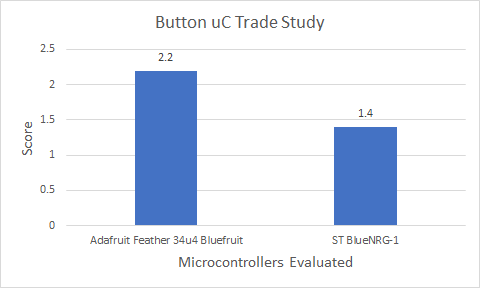
\includegraphics[width=0.4\textwidth]{ButtonTS.png}
\caption{ \space Button Trade Study Results}
\label{HaHa Button TS}
\end{figure}

\begin{figure}[ht] 	% Several different modifiers can be used
\centering
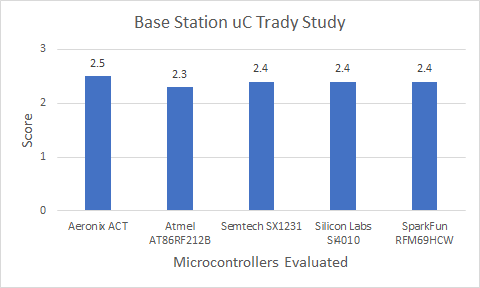
\includegraphics[width=0.4\textwidth]{BaseTS.png}
\caption{ \space Base Station Trade Study Results}
\label{HaHa Base TS}
\end{figure}

\section{System Overview}

\subsection{Product Perspective}
The base station and button will be separate hardware devices which facilitate the communication of a “help request” when a user presses the button on either the base station or the remote button. The base station will contain a priority list of contacts who will be contacted in an order set by the user. Alerted users will respond to the help request through use of their own base station.  If a user does not respond to a help request, the next person on the list is contacted. If none of the people on the help list respond, any station in the nearby vicinity is contacted.

\subsubsection{Design Method}
The software design portion of the product will utilize the C-programming language.

\subsubsection{User Interfaces}
The base station is equipped with an LCD display, which will facilitate user interaction with the device, in addition to showing critical information during emergency situations. Configuration of the device shall be done using a series of menus displayed on the LCD display. The exception to this are several dedicated switches/buttons that control the contrast of the display, reset device power, and trigger the help request functionality. The rest of the device functionality shall be accessed through the menu system, and facilitating this is a set of four directional buttons, as shown in Figure \ref{dev buttons}. These buttons shall have the following functionality:

\begin{LaTeXdescription}
	\item[Up] Scroll up in the list of choices
    \item[Down] Scroll down in the list of choices
    \item[Left] Move back/cancel, exiting a submenu
    \item[Right] Select, selecting the current item (that which is listed at the top of the screeu) or open the corresponding submenu
\end{LaTeXdescription}

\begin{figure}
	\centering
	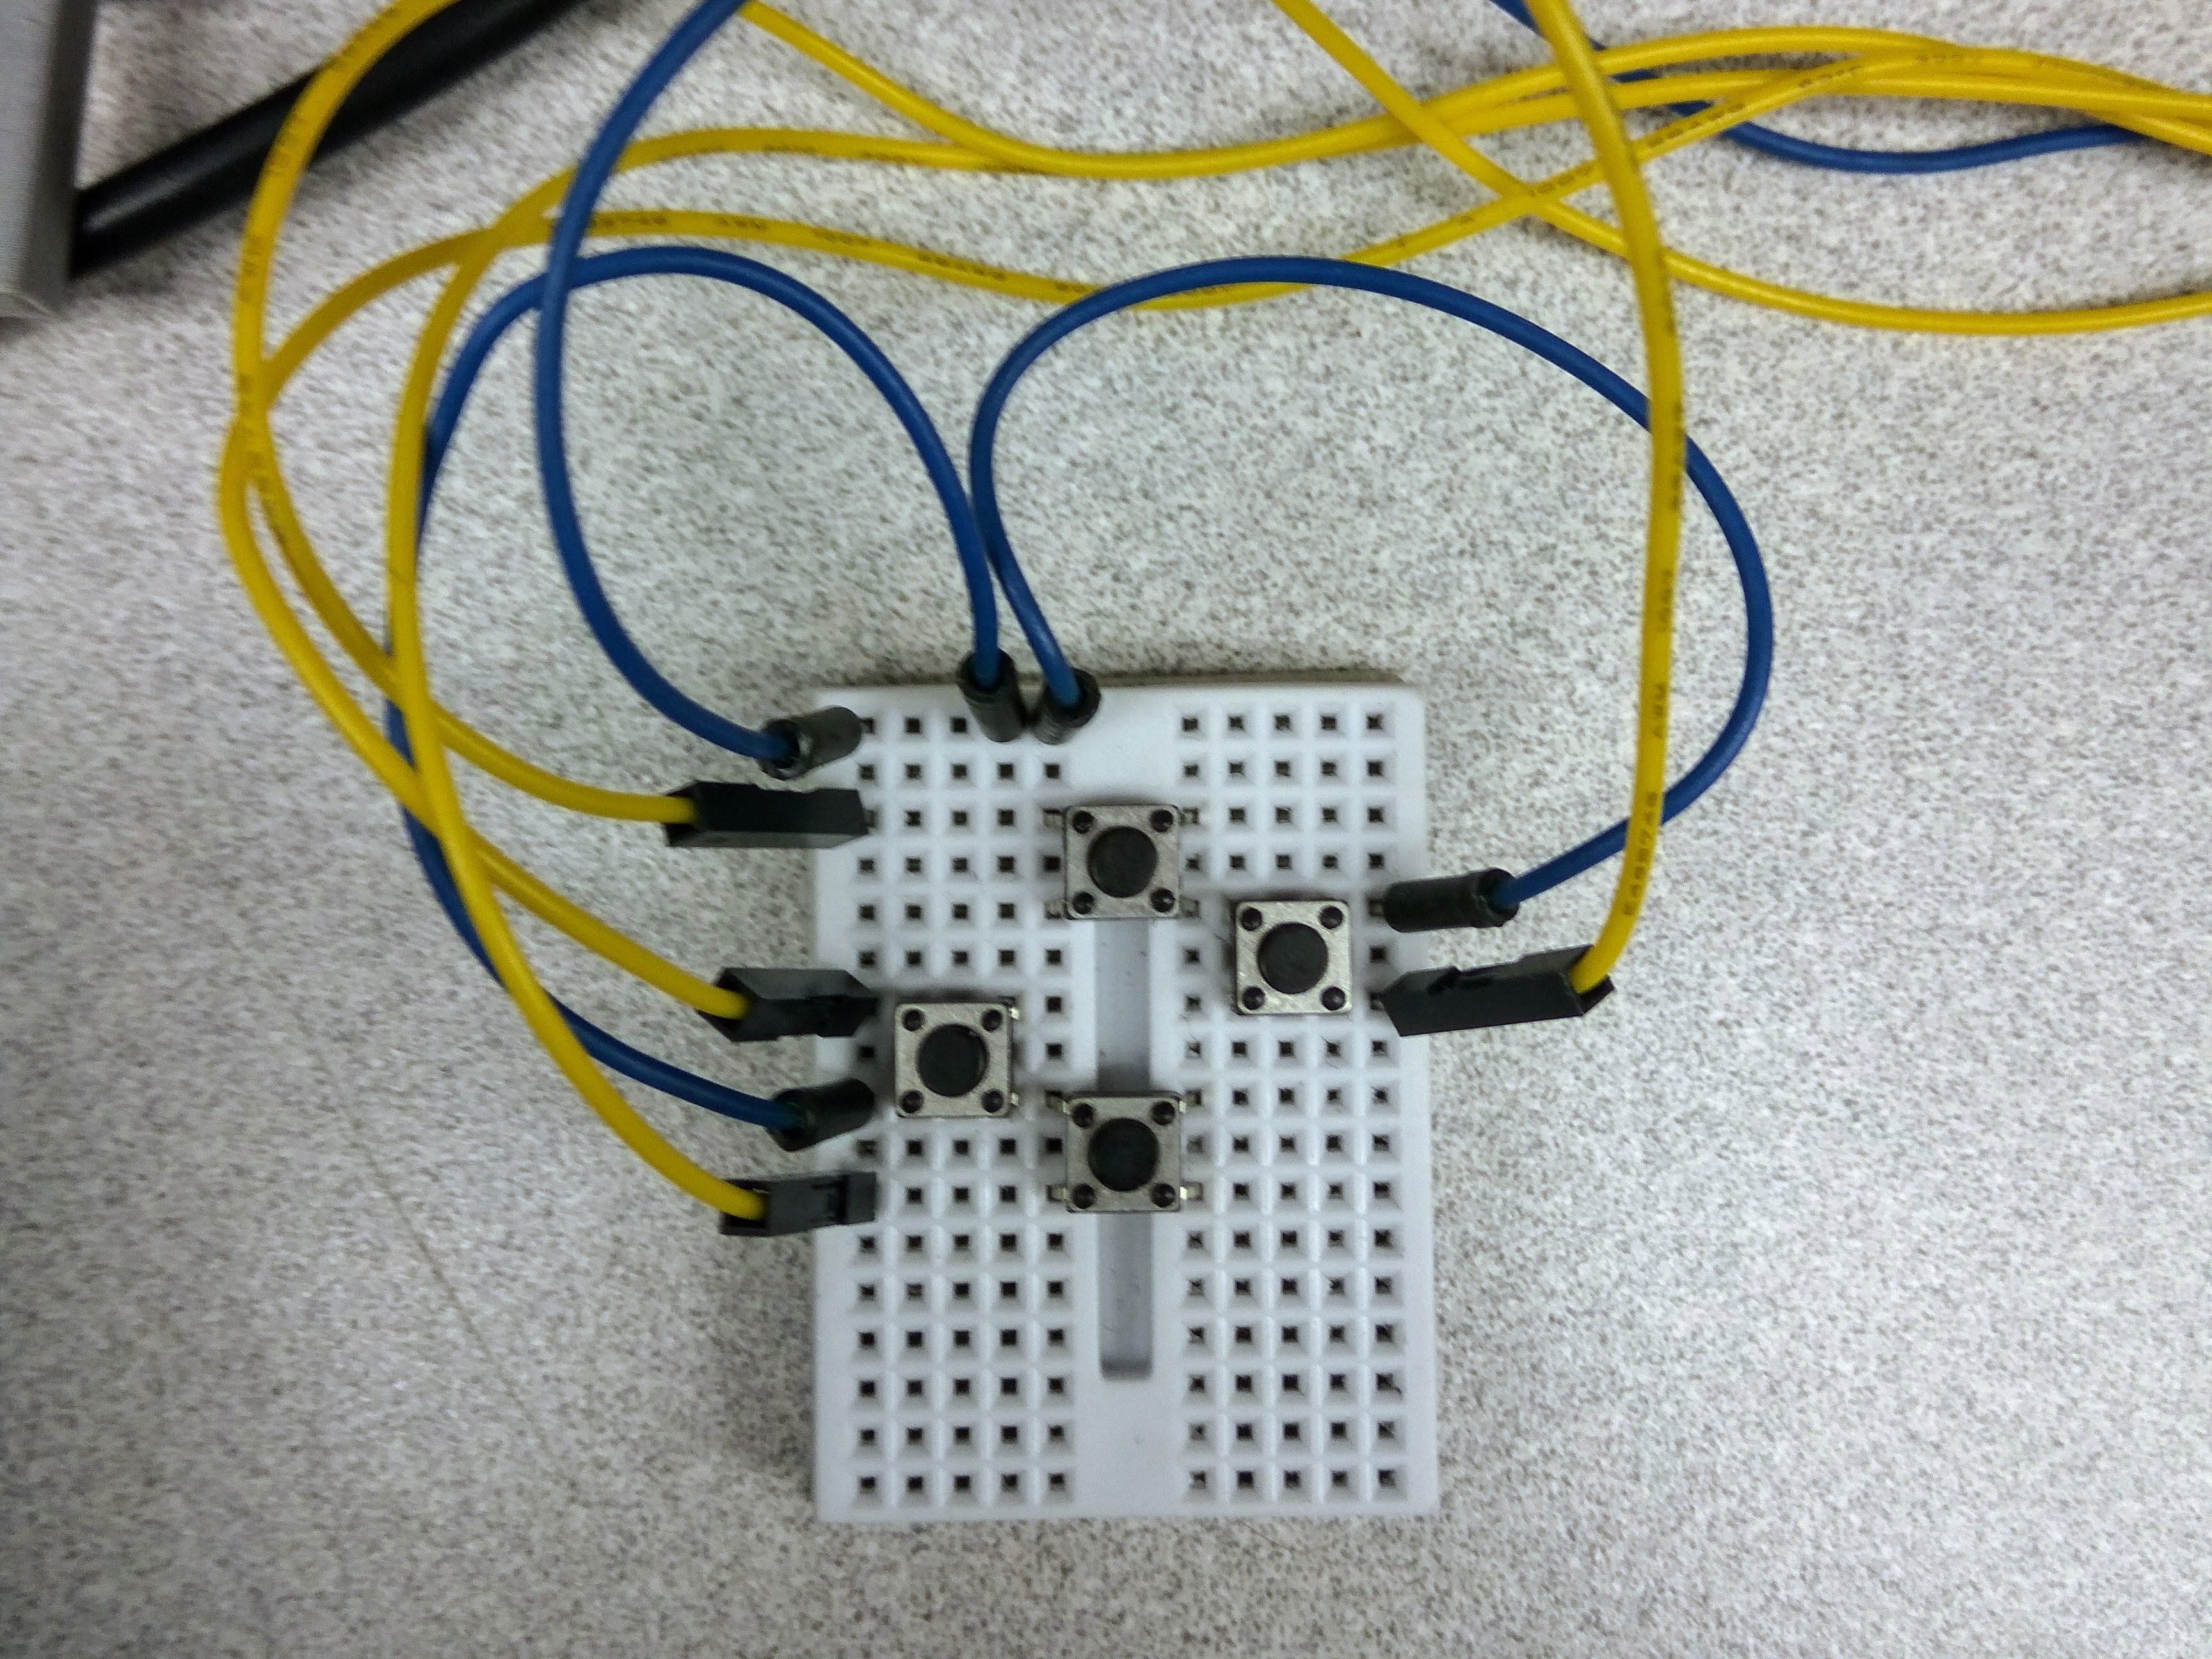
\includegraphics[width=0.48\textwidth]{dev_buttons.jpg}
    \caption{Directional Buttons on the Development Board}
    \label{dev buttons}
\end{figure}

The base station also allows an external device (such as a lamp) to be plugged directly into it. This device will be toggled on and off during emergency situations.

The button is equipped with a single button to trigger the emergency response system. Different inputs (such as a single press, three successive presses, and a hold) serve different functionality. It also has LED indicators for periodic synchronization pulses, confirmations that the help request has been received, and to confirm another user has answered the distress call.

\subsubsection{Hardware Interfaces}
The hardware of the base station and the remote button will be designed and developed by the team.

\subsubsection{Operations}
The user of the base station will be required to setup a priority contact list.  The system will have the option of scanning for all available network nodes which will display the name of nearby users and their node number.  Configuring of a user to contact can also be done via a pre-shared ID number which each base station user can obtain through the user interface.

When a help request is sent, the initiating user will be able to cancel the request by long-pressing the help button either on the base station or remote button.

\subsection{Product Functions}

\begin{LaTeXdescription}
\item[Send Help Request] This function will send a help request beginning with the first base station in the user’s contact list. Functionality for this will be present on both the remote button and the base station.
\item[Cancel Help Request] This function cancels a help request alert. In the event a user has already responded to a help request, an additional signal will be sent to the box of the responder to inform them of the canceled request.
\item[Setup Contact List] This set of functions will facilitate configuring the user’s contact list.  Users can either enter ID numbers of the neighbors they wish to add or they can scan the network for them.
\item[Scan Network] This function scans the network for available users and provides user contact details. It will interface directly with the Setup Contact List.
\end{LaTeXdescription}

\subsubsection{Software}

\subsubsection{Application Networking Protocols}

This section is an overview of the networking protocols which must be determined.  Specific information such as packet design will be fleshed out in the next section, System Architecture.

\begin{itemize}
  \item Button to Box
    \begin{itemize}
      \item Base station reads button battery level using Bluetooth API. (performed frequently)
      \item Button activates “Help Alert” state on the base station. (button pressed for 3 sec)
      \item Button activates “Immediate Help Alert” state on the base station. (button pressed for 6 sec)
    \end{itemize}
  \item Base Station to Base Station
    \begin{itemize}
      \item Discovering neighbors. (broadcast)
      \item Sends help request to specific and possibly distant neighbor. (ACK’d)
      \item Sends help alert received signal back to requester. (broadcast)
      \item Sends help alert resolved signal to all neighbors requested. (broadcast)
    \end{itemize}
\end{itemize}

\subsection{System Diagram}

To meet the desired functions of our product, we generated a high-level block diagram that contains all of the parts that are required for the implementation of the system.

\begin{figure}[ht] 	% Several different modifiers can be used
\centering
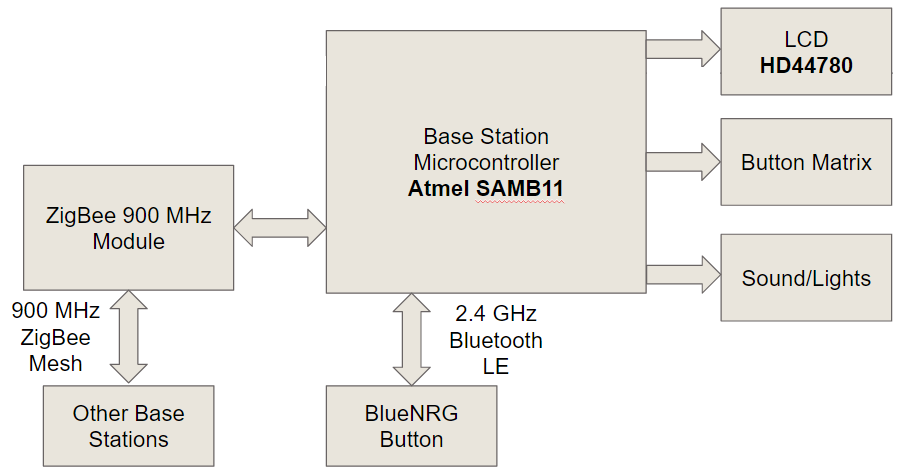
\includegraphics[width=0.4\textwidth]{system_diagram.png}
\caption{Block diagram of the system}
\label{Ha-Ha System Diagram}
\end{figure}

\subsection{Network Simulation}

NS3 is a discrete-event network simulator. A discrete-event are those events which occur in a sequence over time. Each event occurs at a particular instant in time and marks a change of state in the system. NS3 facilitates the defining of this system and mechanisms to view and record the state of every mechanism within the system.

Our goal with NS3 is to simulate the network as closely as possible to the DigiMesh protocol using the AODV algorithm as a basis. Packet broadcasts that approximate our own application layer packets will be configured and the number of nodes scaled such that the network performance can be analyzed as the number of nodes or amount of network traffic increases. This will allow us to realize with some level of certainty the level at which our network will be deployable. It also will provide us with a basis for any future troubleshooting of the network that we might encounter a need for.

In its current form, the simulator creates a configurable number of nodes a random x-y-z distance apart and has the two furthest nodes communicate packets. The communications regarding the AODV algorithm are traced and logged to the screen along with the communication packets. As state above, this will be modified in the coming quarter to be more representative of our system.

Below is an example output:

\begin{lstlisting}
Creating 10 nodes 100 m apart.
x=80.7772, y=45.6102, z=0.458782
x=48.6495, y=72.3938, z=0.448497
x=22.2484, y=53.5658, z=0.513956
x=26.1946, y=19.7807, z=0.446207
x=68.3362, y=54.6383, z=0.830643
x=92.0653, y=28.9132, z=0.773134
x=54.4156, y=93.372, z=0.662756
x=14.7075, y=19.3661, z=0.662903
x=46.9031, y=68.3726, z=0.521647
x=53.8059, y=83.5943, z=0.0441295
Starting simulation for 10 s ...
[node 0] Starting at time 36ms
[node 1] Starting at time 32ms
[node 2] Starting at time 73ms
[node 3] Starting at time 53ms
[node 4] Starting at time 95ms
[node 5] Starting at time 95ms
[node 6] Starting at time 99ms
[node 7] Starting at time 22ms
[node 8] Starting at time 11ms
[node 9] Starting at time 27ms
PING  10.0.0.10 56(84) bytes of data.
[node 0] Valid Route not found
[node 0] Send RREQ with id 1 to socket
[node 6] Starting at time 99ms
[node 7] Starting at time 22ms
[node 8] Starting at time 11ms
[node 9] Starting at time 27ms
PING  10.0.0.10 56(84) bytes of data.
[node 0] Valid Route not found
[node 0] Send RREQ with id 1 to socket
on 10.0.0.10
[node 9] AODV node 0x1bf5760 received 
a AODV packet from 10.0.0.1 to 10.0.0.10
[node 9] Send reply since I am the 
destination
[node 9] Exist route to 10.0.0.1 from 
interface 10.0.0.10
[node 9] Updating VALID route
[node 9] Updating VALID route
\end{lstlisting}

\section{System Architecture}

\subsection{Button Software}

The button and base station are paired together to form a master/slave relationship where the button is the slave and the base station the master.  The button transmits signals to the base station in the form of packets.  After receiving a packet, the base station processes the information accordingly to either forward the message to other base stations or back to the button.  The button is usually in sleep mode and only wakes up if a button event occurs.  The following cases are envisioned requirements to be fulfilled by the respective hardware component’s libraries.

\begin{LaTeXdescription}
\item[Case 1]: Initial connection established between button and base station.
  \begin{itemize}
    \item The button device is initially in standby mode waiting to be paired.  The button is pressed on the base station to establish the initial connection process.  The button on the button device is then pressed and held for a several seconds until a message appears on the base station confirming successful connection.  This initial process only occurs once when a single button device is registered to a base station.
  \end{itemize}
\item[Case 2]: The button is pressed within range of the base station.
  \begin{itemize}
    \item The button can either send a help alert signal or cancel a help alert packet.
    \item If the button is pressed and held down for 3 seconds, it will transmit a help alert packet to the base station.  After acknowledging a help alert packet was received, the base station will transmit the help alert to the contacts listed in the requester’s network list.  If the first person on the list does not respond within a certain timeframe, it will timeout and go to the next contact on the list.  If no one on the list responds, then the packet is sent to additional neighbors.  If none of these additional neighbors respond, the packet is then sent through a certain number of network hops which will be calculated according to the density of base stations existing base stations.  If no one still responds, then the packet is sent through the entire network of base stations as a final pass.
    \item If the button is pressed 3 times consecutively, then it will transmit a cancellation of the help request packet.  After receiving and acknowledging this type of packet was indeed received, it will cancel the help request.  There will be a help request cancellation message displayed on the base station.
  \end{itemize}
\item[Case 3]: The button is pressed when out of range of the base station.
  \begin{itemize}
    \item If the button is out of range of the base station, it will disconnect and won’t be able to transmit or receive any packets.  Once it is back within range of the base station, it will automatically connect to it and a successful connection message will be displayed on the base station.
  \end{itemize}
\item[Case 4]:  The button is not pressed but wakes up to send notifications to the base stations within range.
  \begin{itemize}
    \item The base station continually polls information from the button.  The percentage of the button’s battery life is polled by the base station for a given amount of time.  Another query occurs every 6 hours to determine if the button is still connected to the base station.  If base station does not receive a signal from the button within 12 hours, it will notify the user there is an issue with the button by displaying this information on the base station.
    \item When the battery is drained under a certain percentage, it would notify the user the battery is low.  A message will be displayed on the base station informing the user to replace the button battery.  The LED on the button will also become a solid red color to signal the low battery life and it will eventually begin blinking if the battery life is critically low and in need of immediate replacement.
  \end{itemize}
\item[Case 5]: The button is not pressed but wakes up to send notifications to base stations not within range.
  \begin{itemize}
    \item Same conditions as Case 3.
  \end{itemize}
\end{LaTeXdescription}

\subsection{Base Station Software}

\begin{figure}[ht] 	% There are several different modifiers that can be used in [].
\centering
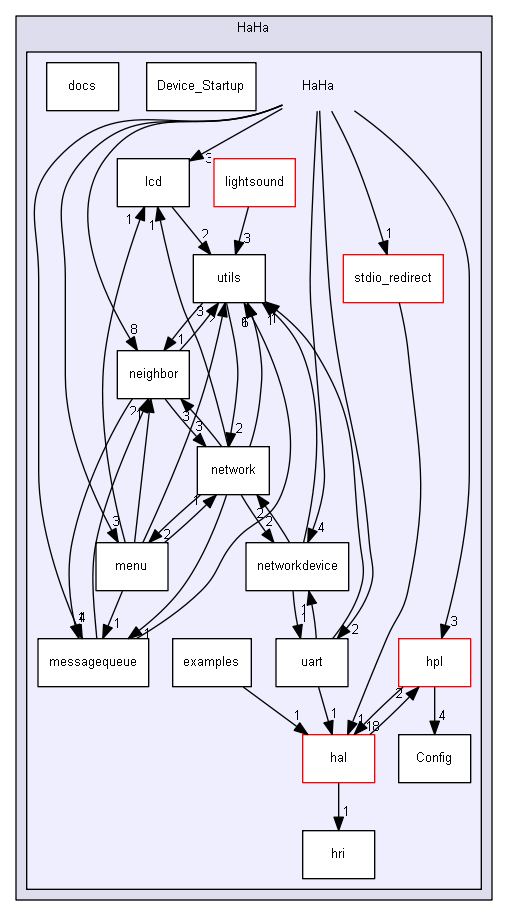
\includegraphics[width=0.4\textwidth]{hahamap.png}
\caption{ \space Software map.}
\label{HaHa Application}
\end{figure}

\subsubsection{Application Modules}

As can be seen by the UML layout in Fig. \ref{HaHa Application}, our application will be a series of modules meant to interconnect and provide the needed functionality. By creating modules for each portion of software it will be possible for modifications to be easily implemented by replacing the relevant modules. This project is being developed as an open-source project and as such it is our endeavor to allow modifying the system easy and straightforward.

Chief among this modularity is the “network device” layer we are developing to utilize a Digi ZigBee module. This layer and its modules will be responsible for receiving data in the form of a character string from the upper application and converting it as necessary to be sent as an XBee network frame. On the receiving end it will do the reverse operation and provide the upper layer with a character string. In the event that a different transceiver wished to be used, creating and implementing similar functions would allow the majority of the application layer to remain unmodified.

\subsection{Graphical User Interface}
\subsubsection{Display}

The base station was equipped with a Crystalfontz CFAH1604A-TMI-JT 16x4 LCD display. A 4 line display was a requirement for the project, as the device would be used during high stress situations, in which users would want to see all necessary information on one screen without having to interact with the device interface. The Crystalfontz display was the cheapest 4 line display available find on the market, and had the added benefit of being based off of the Hitachi HD44780U, a widely used and well documented component.

Similar to other software components in the project, we abstracted the display drivers into two separate modules, a device specific component and a generic component:

\begin{LaTeXdescription}
	\item[lcd\_device] holds device specific code and macros, such as the display size (\lstinline[columns=fixed]{LCD_ROWS=4, LCD_COLS=16}), and facilitates the communication with the physical device, which in this case means writing to specific registers
    \item[lcd] abstracts the physical device, by buffering the output to the LCD screen with arrays implemented in software. A single \lstinline[columns=fixed]{lcd_update} function updates the entire LCD screen contents.
\end{LaTeXdescription}

There were some complications with implementing the LCD driver. First is the subtle differences between the Crystalfontz display and the Hitachi specification. After the initial version of the driver was implemented, we noticed that the display would only work correctly if the delay in between commands was set to more than 90 ms. This was unusual, as the datasheet only required a delay of around 40 ms in between commands during the initialization phase, and then 3 ms when writing to the screen. We eventually discovered that this was due to the Crystalfontz controller expecting a specific initialization command to be sent twice, which was only briefly mentioned on their datasheet and was not part of the Hitachi specification at all. This forced us to use the Crystalfontz datasheet for the rest of development, which was overall not as intuitively laid out as the one given by Hitachi. 

Another design decision in integrating the LCD display was to use 4 bit mode, as opposed to 8 bit mode. 8 bit mode is standard, in which each character is specified in 8 bits, which is standard ASCII. 4 bit mode sets the controller to read in only 4 bits of data at a time, thus requiring two register writes per character/command to 8 bit mode's 1 write. The justification for doing so was to free up pins on the microcontroller, which had many components to interface to. In addition to the 4 data pins, the LCD display already required 3 pins for control, making it the largest component in terms of pin usage. However, this had some drawbacks, in both development and performance. The Crystalfontz datasheet had minimal examples for operating in 4 bit mode, which meant that each 8 bit command had to be "translated" into 4 bit commands, which was tedious and hindered the progress of debugging. On the performance side, since each command took twice as many writes, when compounded with the mandatory delay between commands, this produced noticeable lag when communicating 

Besides the obvious benefit of being able to swap out the device specific code as necessary, there was a very specific reason the \lstinline[columns=fixed]{lcd} module needed to buffer the LCD output, having to do with the way the LCD controller operated specifically for a 16x4 display. In a standard 16x2 display, the controller would read in 16 characters corresponding to the top line of the display. It would then expect a command to change the write address to the second row, and take in an additional 16 characters. However, for a 16x4 display, the same controller was adapted to work in a similar way. In order to accomplish this, the third and fourth rows are simply extensions of the first and second rows, resulting in the following unusual behavior: writing 16 characters for the first row, then 16 characters for the third row, followed by the address command and following 16 characters for the second then fourth rows respectively. What this means in practice is that the LCD display cannot support writing characters in order, which makes buffering necessary in order to implement functions such as \lstinline[columns=fixed]{lcd_set_line()}.

\subsubsection{User Interface}

The user interface of the base station is composed of a tree of menu items, a data structure defined in the \lstinline[columns=fixed]{menu} software module (included in Appendix \ref{MenuItem Code}). Each menu item has reference to it's parent, it's next and previous sibling, and it's first child, all of which are also menu items. These four references relate to the four cardinal directions given in the user interface:

\begin{LaTeXdescription}
	\item[Up] Scrolls up in the current list of menus, setting the cursor as the previous sibling of the current item (or if current is the first sibling, to it's last sibling), and then calling it's \lstinline[columns=fixed]{onView()} method.
    \item[Down] Scrolls down in the current list of menus, setting the cursor as the next sibling of the current item (or if current is the last sibling, to it's first sibling), and then calling it's \lstinline[columns=fixed]{onView()} method.
    \item[Left] Moves back (up) in the menu tree, setting the current item as the parent and then calling it's \lstinline[columns=fixed]{onView()} method.
    \item[Right] Selects the current item, calling it's \lstinline[columns=fixed]{onClick()} method. By default, this sets the cursor to the child of the current item, if it exists.
\end{LaTeXdescription}

Referenced above, each menu item also has two function callbacks assigned to it, which are referred to as the \lstinline[columns=fixed]{onView()} and \lstinline[columns=fixed]{onClick()} methods. These functions are called throughout the menu navigation process, and are what allow the menu to dynamically alter both itself and the other software modules of the base station. 

The \lstinline[columns=fixed]{onView()} method is called whenever a menu is viewed. By default, this takes form of printing the current menu item's string \lstinline[columns=fixed]{value} on the top line of the LCD screen, with it's next siblings shown on the following lines, as seen in Figure \ref{menu view default}. This gives the user context as to what they are currently selecting, and what is available to be selected should the user choose to move up/down. However, there are some cases where this is not ideal, such as in the User Info submenu. Because some fields of user information typically span more than one line (the address field specifically is a good example of this), each child of the User Info menu item has a custom \lstinline[columns=fixed]{onView()} callback, which takes up the entire screen. Pressing up and down for this submenu still navigates between items, but overwrites the entire screen, like shown in Figure \ref{menu view user info}. In addition, the second line of the LCD screen is populated with user info taken from a datastructure defined in another software module. Another custom \lstinline[columns=fixed]{onView()} method is used in the text input feature, which will be discussed in greater detail later.

\begin{figure}
  \begin{subfigure}{0.48\textwidth}
  	\centering
    \LCD{4}{16} |Friends List   >|
                |User Info       |
                |Device Settings |
                |                |
    \caption{Default View}
    \label{menu view default}
  \end{subfigure}
  \begin{subfigure}{0.48\textwidth}
    \centering
    \LCD{4}{16} |USER ADDRESS:   |
                |1157 High St. Sa|
                |nta Cruz, CA    |
                |vMore      Edit>|
    \caption{User Info Custom View}
    \label{menu view user info}
  \end{subfigure}
  \caption{\lstinline[columns=fixed]{onView()} methods}
\end{figure}

As mentioned in the table, by default, the \lstinline[columns=fixed]{onClick()} method of a menu item should navigate to it's corresponding submenu (it's first child). However, there are some situations where it is necessary to do more. For example, every time the Friends List menu item is clicked, it's children are regenerated based on the current state of the software friend list. The end result is the same (the cursor being set as the first friend in the list, which is the first child of the Friends List menu item), but because other actions are going on in the background to produce these children, the \lstinline[columns=fixed]{onClick()} method had to be overwritten. Another good example is again the User Info items mentioned previously. Selecting them starts the text input feature, which creates a large subtree below the current item.

The Help Request and Friend Request features use a combination of the \lstinline[columns=fixed]{onView()} and \lstinline[columns=fixed]{onClick()} methods to provide a cohesive message. When a request is received over the network, the cursor is forcibly set to the menu item Help Response, with the view method producing a screen like that shown on Figure \ref{menu view help}. This method, similar to the User Info menu item, takes in a name (this time from a network packet) and displays it on the screen. The resultant menu tree after this process is completed looks like this:

\begin{itemize}
	\item Help Response Root
    \begin{LaTeXdescription}
        \item[child] Help Response Deny
        	\begin{LaTeXdescription}
                \item[onClick] NULL
                \item[onView] Send "Cannot help you" packet, set current to root
                \item[child] Help Response
                    \begin{LaTeXdescription}
                        \item[onClick] Send "Help is on the way" packet, set current to root
                        \item[onView] Show information on the person who needs help (see Figure \ref{menu view help})
    				\end{LaTeXdescription}
            \end{LaTeXdescription}
    \end{LaTeXdescription}
\end{itemize}

\begin{figure}
  \begin{subfigure}{0.48\textwidth}
  \centering
  \LCD{4}{16} |! HELP REQUEST !|
              |Donald Wiberg   |
              |                |
              |<BACK   RESPOND>|
  \caption{Help Request Text}
  \end{subfigure}
  \begin{subfigure}{0.48\textwidth}
  	\centering
  	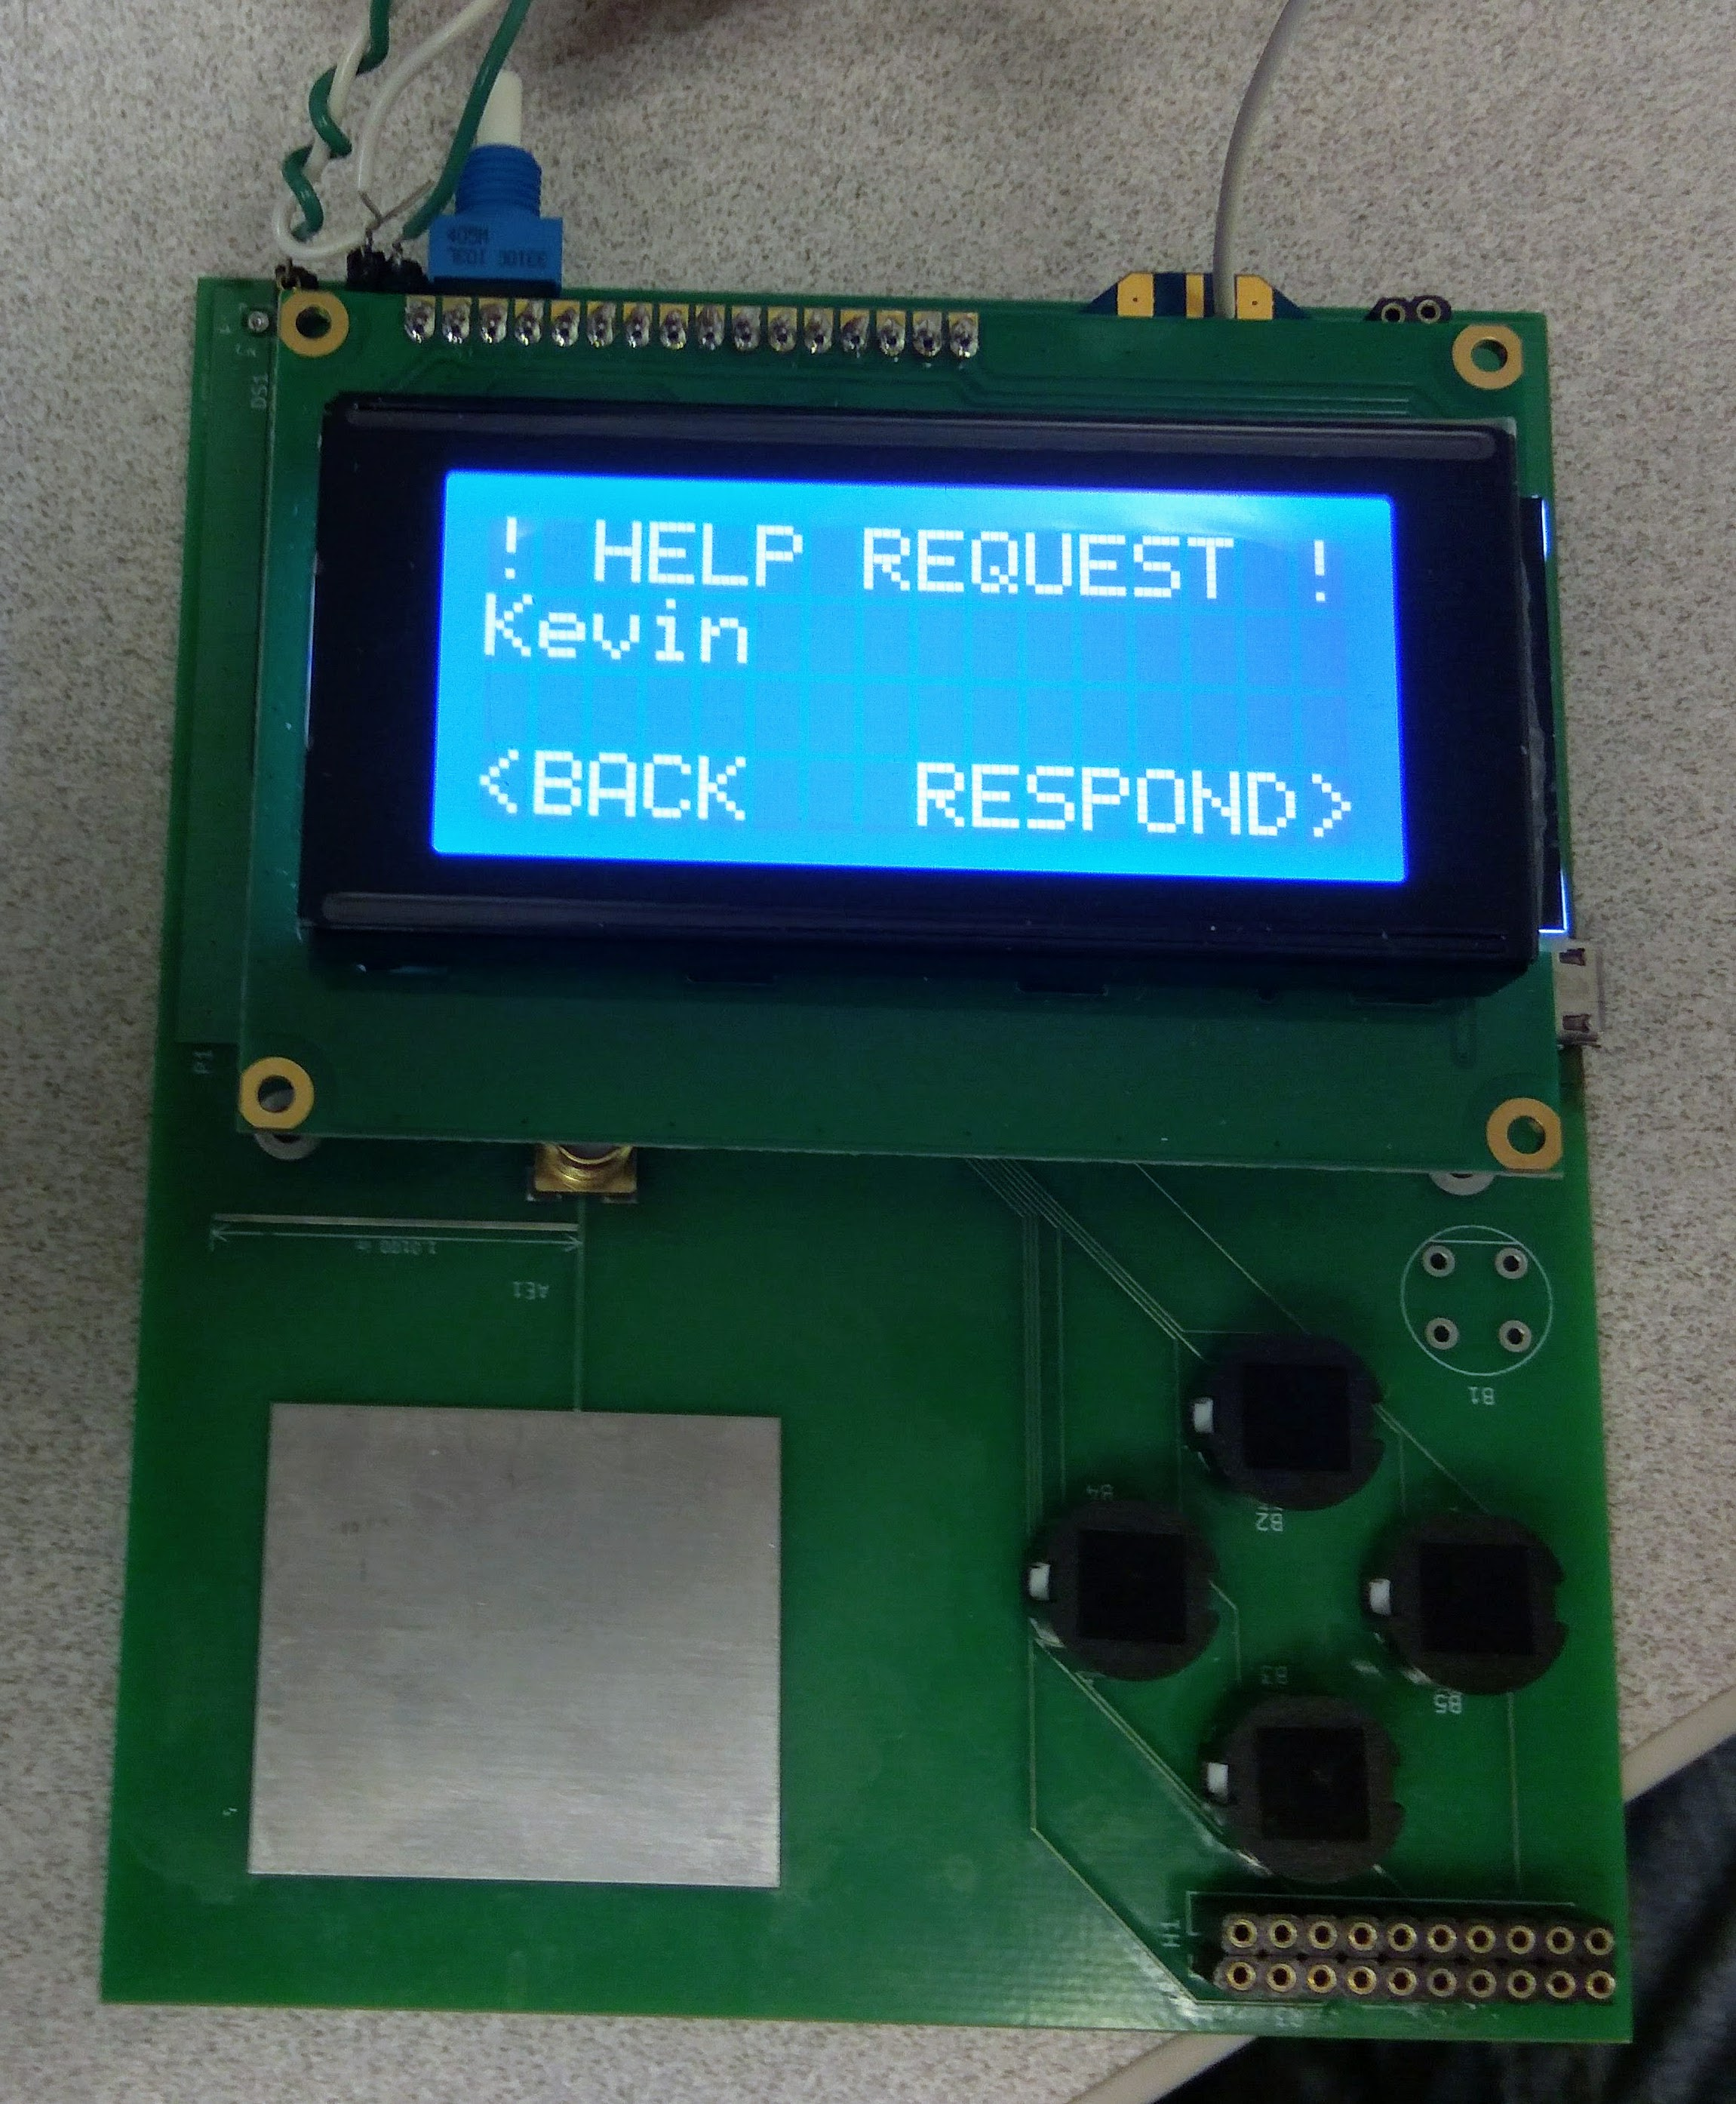
\includegraphics[width=\textwidth]{device_help_request.jpg}
    \caption{Help Request on Physical Device}
  \end{subfigure}
  \caption{Help Request View}
  \label{menu view help}
\end{figure}

Thus, when the user presses right, the click method of Help Response is called, and the affirmative packet is sent. Likewise, if the user presses left, then the menu transitions to the Help Response Deny (which is the parent of the Help Response menu item), and it's view method is called. This causes the negative packet to be sent. In either case, the user is immediately transitioned back to the root menu item, which is the default startup screen.

\subsubsection{Text Input}

The base station facilitates text input much the same way as a networked printer or old school arcade game would. Up (Figure \ref{menu input up}) and down (Figure \ref{menu input down}) changes the current letter at the cursor, left (Figure \ref{menu input left}) deletes a character, and right (Figure \ref{menu input right}) selects the current character displayed. Depending on the context of the text input, the characters available may differ. For instance, names support upper case and lower case letters, in addition to spaces, which when scrolling through the list of letters is represented by an underscore. Likewise, addresses support only upper case letters to limit complexity, but also include spaces, numbers, and periods. Lastly, phone numbers only support numbers. In all cases, when scrolling through the list of characters, there is the addition of a special character, the right arrow ($\rightarrow$). This represents the enter key, and signifies that the user is finished with the string they are editing and would like to save. Deleting the entire string, and then continuing to press left exits the editor, discarding changes.

\begin{figure}
  \begin{subfigure}{0.48\textwidth}
  	\centering
    \LCD{4}{16} |Editing Name:  >|
                |STEPHEN PETERS  |
                |                |
                |                |
    \caption{Initial State}
    \label{menu input start}
  \end{subfigure}
  \begin{subfigure}{0.48\textwidth}
  	\centering
    \LCD{4}{16} |Editing Name:  >|
                |STEPHEN PETERR  |
                |                |
                |                |
    \caption{Up Press (prev letter)}
    \label{menu input up}
  \end{subfigure}
  \begin{subfigure}{0.48\textwidth}
  	\centering
    \LCD{4}{16} |Editing Name:  >|
                |STEPHEN PETERT  |
                |                |
                |                |
    \caption{Down Press (next letter)}
    \label{menu input down}
  \end{subfigure}
  \begin{subfigure}{0.48\textwidth}
  	\centering
    \LCD{4}{16} |Editing Name:  >|
                |STEPHEN PETE_   |
                |                |
                |                |
    \caption{Left Press (delete letter)}
    \label{menu input left}
  \end{subfigure}
  \begin{subfigure}{0.48\textwidth}
  	\centering
    \LCD{4}{16} |Editing Name:  >|
                |STEPHEN PETERS_ |
                |                |
                |                |
    \caption{Right Press (confim letter)}
    \label{menu input right}
  \end{subfigure}
  \caption{Text Input States}
\end{figure}
\begin{comment}

\textbf{User Interface}

The base station design was motivated by two primary goals: (1) to be easy and intuitive for elderly people to operate in emergency situations, and (2) to be composed of inexpensive components to support wide adoption by the community.  These goals were somewhat contradictory: inexpensive components are often the most difficult to work with, while better components are more expensive which will drive up the overall cost of the system.  Our sponsor, Professor Emeritus Donald Wiberg, gave us a soft limit of approximately \$50 for the entire system’s components (not including packaging), which greatly limited which components were feasible for our project.

Thus, it was our decision to make the base station’s interface as easy to use as possible, which made it critical that the user interface software be as simple as possible. This requires minimizing the amount of input the user can provide, to make it immediately apparent what is expected of them in order to perform a certain action.  This has the additional effect of minimizing our state machine, which should make programming the device much easier.

The base station is equipped with 5 buttons, which serve the following purposes:

\begin{LaTeXdescription}
\item[Up] Move up in the list of menu items
\item[Down] Move down in a list of menu items
\item[Left/Back/Cancel] Cancel action and move back in the menu tree
\item[Right/Forward/Select] Select the current menu item (the one displayed the top of the screen), and perform said action/move into said submenu
\item[Help Request] Trigger the emergency request system, performing the same functionality as pressing your Bluetooth button
\end{LaTeXdescription}

The LCD screen displays a list of menu items for the current view, in standard operation.  These menu items can be thought of as (possibly selectable) options which the user can place their cursor on.  In the system, the cursor, or “currently selected item”, is the topmost item in the list.  Below the cursor is a variable length list of other viable options which can be scrolled through using the up and down buttons.  Moving your cursor shifts the entire list up or down one space and the lists have currently been configured to wrap around at the end, moving back to the top upon reaching the bottom (but can be easily configured to not do so).  If the cursor is selectable, then the last character of the line is the “>” character, to signify a right button press will select that item. Selectable items that are not currently the cursor have the arrow “→” character as their last character to indicate as such. The back arrow will navigate to the current item’s parent and exit the existing submenu.
\end{comment}

\subsection{Network Application Layer}

The Application Layer between base station communications has several different commands which can be transmitted.  Most of these events are triggered by the user but since multiple users can contact any station at any time, we need a robust way to handle each request. 
Each station will have a packet queue where it can send packets and expect to receive packets from the destinations in which they were sent.  These queues will have timeouts to protect the integrity of the device as well as allowing communication between devices.

\subsubsection{Network Adaptation Layer}

The network adaptation layer is a module that isolates the HaHa application from the network being used to transmit data between the base stations. 

\begin{figure}[ht] 	% There are several different modifiers that can be used in [].
\centering
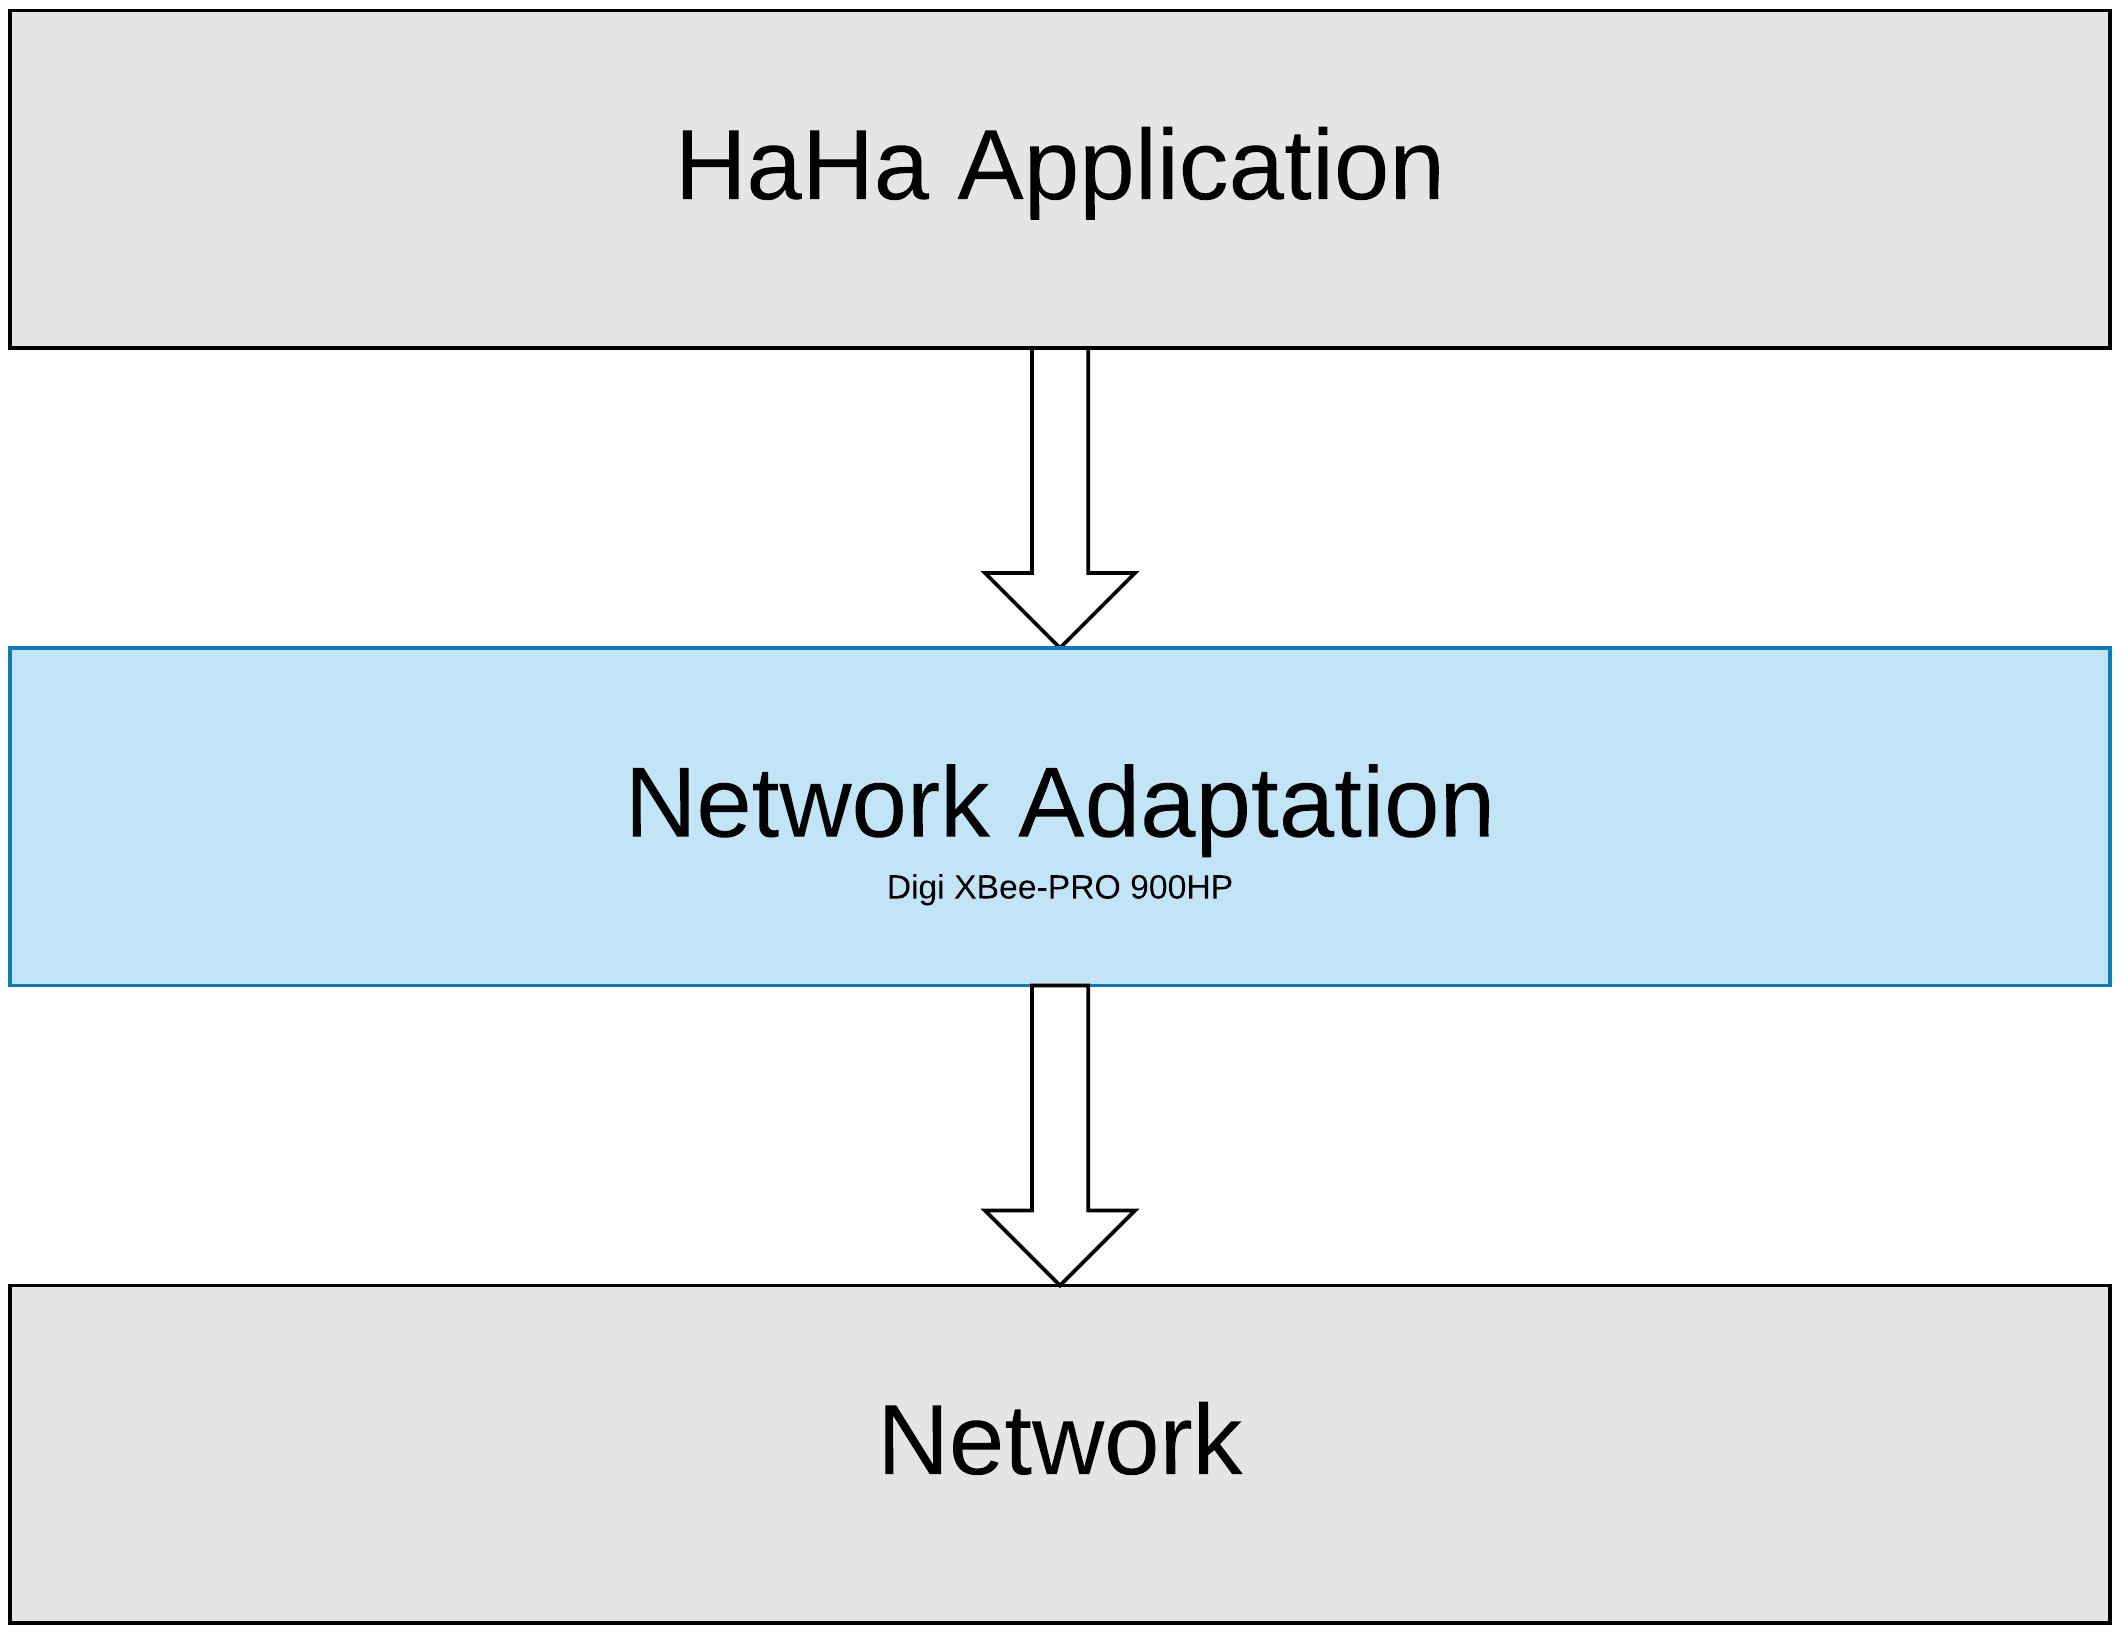
\includegraphics[width=0.4\textwidth]{NetAdaptation.png}
\caption{ \space Network adaptation layer.}
\label{Network Adaptation}
\end{figure}

By implementing the externally accessible functions contained in the {\it networkdevice} files, the network communication device and protocols can be modified or replaced. The functions for a new device need only accept the appropriate parameters and return the expected data types in order to effectively change the any aspect of the communication device or the network medium or protocol.

The network adaptation layer API uses callback functions to route an incoming application packet. By registering the appropriate callback, during receipt any of application packets are directed to their appropriate application handler. This ability to redirect any incoming packet reinforced the modular design. Appendix \ref{appendixnetadapt} lists the required minimum functions to be implemented for any network device to integrate with the HaHa application.

For each received packet from another user base station, the source network address was extracted from the frame packet and sent to the HaHa application. Processing of the source network information in this layer allowed the application to accept any type of network layer with respect to future modifications.

The modular design approach was utilized during the development of this project. It became necessary to implement a logging feature for use in a concept deployment study. Because the network functionality was completely separate from the rest of the application, the implementation of a {\it catch-all} mechanism was efficiently implemented and without change to the core HaHa application, except for a modified receiver running a modified code-base to store the data.

\subsubsection{Frame Structure}

The network adaptation layer currently supports the Digi Xbee 900HP module. Table \ref{digiframe} shows the frame packet structure. Different types of XBee frame packets were implemented to provide the following functionality: transmit (TX), receive (RX), TX Status, Command, and Modem status. Each of these types were contained inside of the Frame Data field, with each the TX and RX frames being a container for the HaHa application packets.

Each frame received was parsed for its type on receipt. A lookup table determined which frame handler to send the frame for handling of its data field. Not all incoming frames were redirected to the application. The TX Status and Modem status frames were handled by the adaptation layer in order to provide the application with network status information. This method allows for the exact mechanism for this information collection to be changed without modification of the HaHa application.

\begin{table}[]
\centering
\begin{tabular}{ccccc}
\hline
\multicolumn{1}{|c|}{1 Byte} & \multicolumn{1}{c|}{1 Byte} & \multicolumn{1}{c|}{1 Byte} & \multicolumn{1}{c|}{variable Byte} & \multicolumn{1}{c|}{1 Byte} \\ \hline
        START  &  Length &    Length     &    Frame Data    &  Checksum  \\
        Delim  & MSB     &      LSB      &                  &            \\
\end{tabular}
\caption{Frame Structure}
\label{digiframe}
\end{table}

\subsubsection{Packet Structure}

%\begin{sidewaystable*}[t]
\begin{table*}[t]
  \centering
  \begin{tabular}{>{\bfseries}l|l l l}
    Name & OPCODE (1 byte) & Flags (1 Byte, 8 flags) & Data (2-98 Bytes) \\
    \hline
    PING\_REQUEST & 0x01 & ACK & DESTUID \\
    ACK PING\_REQUEST & PING\_REQ & ACK & SRCUID, SRCNAME \\
    HELP\_REQUEST & 0x02 & ACK|CANCEL|IMM & SRCUID, HOME, PHONE \\
    ACK HELP\_REQUEST & HELP\_REQ & ACK|CANCEL|IMM & SRCUID \\
    HELP\_RESPONSE & 0x03 & ACK|ACCEPT & SRCUID \\
    ACK HELP\_RESPONSE & HELP\_RESP & ACK|ACCEPT & SRCUID \\
    HELP\_FROM\_ANYONE (BRDCST) & 0x04 & CANCEL|IMM & SRCUID, TTL, SRCNAME \\
    HELP\_FROM\_ANYONE\_RESP & 0x05 & ACK|ACCEPT & SRCUID, DESTUID, SRCNAME \\
    ACK HELP\_FROM\_ANYONE\_RESP & HELP\_FROM\_ANY\_RESP & ACK & SUID, DUID, HOME, PHONE \\
    FIND\_HOPS\_REQUEST (BRDCST) & 0x06 & ORIGINUID \\
    FIND\_HOPS\_RESPONSE & 0x07 & ACK & SRCUID, ORIGINUID \\
    ACK FIND\_HOPS\_RESP & FIND\_HOPS\_RESP & ACK & SRCUID, DESTUID \\
    FIND\_NEIGHBORS\_REQ (BRDCST) & 0x08 & ORIGINUID \\
    FIND\_NEIGHBORS\_RESPONSE & 0x09 & SRCUID, ORIGINUID, SRCNAME \\
    ACK FIND\_NEIGHBORS\_RESPONSE & FIND\_NEIGHBORS\_RESP & ACK & SRCUID, DESTUID \\
    FRIEND\_REQUEST & 0x0A & SRCUID, DESTUID, SRCNAME \\
    ACK FRIEND\_REQUEST & FRIEND\_REQUEST & ACK & SRCUID, DESTUID, SRCNAME \\
    FRIEND\_RESPONSE & 0x0B & ACK|ACCEPT & SRCUID, DESTUID \\
    ACK FRIEND\_RESPONSE & FRIEND\_RESPONSE & ACK & SRCUID, DESTUID \\
    UNFRIEND\_REQUEST & 0x0C & SRCUID, DESTUID \\
    ACK UNFRIEND\_REQUEST & UNFRIEND\_REQUEST & ACK & SRCUID, DESTUID
  \end{tabular} \linebreak
  \caption {Base-to-Base Packet Structure}
  \label{Packet Table}
\end{table*}
%\end{sidewaystable*}

Table \ref{Packet Table} lists the entire packet structure for the base-to-base communications.  It is set up to take under 100 Bytes to transmit the entire payload for each packet type, which is the maximum payload of a ZigBee transmission using our transceiver. Any size greater will cause packet fragmentation, in which we would have to reassemble the packets at the destination. An in-depth description of all of the packets can be seen in Appendix \ref{Packet Descriptions}.

The packets which allow users to connect to one another include the FIND\_NEIGHBORS\_REQUEST, which polls the area for contacts.  This will allow the user to locate their individual friends who are nearby as well as individually connect to people who are not within range, providing they are on the same network.

The FRIEND/UNFRIEND packet allows friends to connect to a base station and provides for help requests to be sent.

The main packet driving the system's purpose is the HELP\_REQUEST packet.  If two devices are paired, they can send these packets to one another.  When a help request is sent, it is immediately acknowledged, flags are set within the paired system, and a call to action takes the form of various peripherals with flashing lights and generated noise to signal the friend has requested assistance.  The only way to turn it off is to wait for it to timeout or respond with an accept/reject acknowledgement.  If it does timeout, additional friends on the list are contacted until the list is exhausted.

The HELP\_FROM\_ANYONE Request, which in conjunction with the FIND\_HOPS packet types, allows the base station to request help based on proximity to the station.  This is only used if no friends can answer the original alert request.

\subsubsection{Basecomm}
The base communication file is the packet conversion tool which converts data from the network into packets, as well as packets into data which can be sent on the network. Each converting function prepares all of the required fields based on the packet type, and a helper function copies all of the necessary fields into the application packet. This was originally developed during the Linux testing phase, where we used a different networking protocol, TCP/IP, to send these packets over the network. This was somewhat successful in the Linux Version, as the Network Adaptation Layer to simulate a Zigbee-like network was written only worked on a specific Ubuntu virtual machine. This however proved the concept of the Network Adaptation Layer, which we used in the final build of the system, using the actual hardware rather than a Linux simulation.

\begin{figure}[ht] 	% There are several different modifiers that can be used in [].
\centering
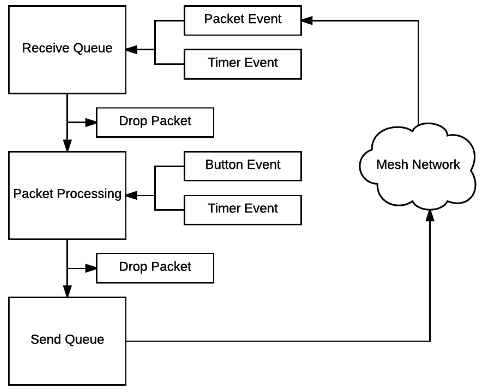
\includegraphics[width=0.4\textwidth]{MessageQueueFlowchart.png}
\caption{ \space Flow of packets to be processed and sent through the message queue system.}
\label{Message Queue Flowchart}
\end{figure}

\subsubsection{Message Queue} 
The goal of the message queue system was so messages sent throughout the network to different stations would be validated before being processed. This means that anyone that connects to the network, including malicious or disruptive users, would have their data validated, and minimize the effects of said malfunctioning devices or malicious users. As shown in Figure \ref{Message Queue Flowchart}, it can be seen that the receive queue of the Message Queue system first inspects the packet for any network issues. If the packet was destined for the device, and the device is expecting the packet, it leads into the Packet Processor. The packet processor has the ability to process as well as send out packets, as well as take input from the user or timer events to refresh old data and test connections between other stations. These items are then sent to the send queue, which will then send it out to the network to other base stations. Though not all of the functions in messagequeue we envisioned ended up being fully implemented, it was a good way to access the packet flow of the system, and to make it less likely to have unnecessary complications later down the road. The main function that was not implemented in the message queue system was the reloading of the system packet responses upon a crash or reboot, which is explained later in the storage section.
\subsubsection{Packet} 
The packet file is used to handle all of the incoming packets, as well as having functions to send packets, which may be called by the user interface, packets, or as a timer event. All of the messaging state processing is handled in this file. The handlers are registered in a function pointer array, and then processed into application packets via a packet converter, which parses the raw packet data from the network layer into an application packet.\newline
Each handler is given the packet, which contains the packet information, as well as an identification number for the network information from which the packet was received from. Some of this data is the time to live on the packet, the source address and destination address. The time to live can be used to determine the number of hops, or physical network devices it took for the packet to arrive at the station, which is what we use it for.
\subsubsection{Neighborlist} 
The purpose of the neighbor list module is to allow for the device to populate a list of nearby base stations, also known as neighbors, which would allow for the user to become friends with those different stations, and thus their users. This list is displayed on the graphical user interface after the neighbors are polled using the find neighbors packet types. To connect to their neighbors, they would go to the add friend menu, which would populate the list with all stations on the network. The user can then send friend requests to these users. This system can also be used to probe the network for the purposes of minimizing large overly large numbers of broadcasts, to keep any broadcasts as physically local to the station, to improve network stability as well as reduce excessive alarms in the help from anyone request, which has the potential to reach a large amount of people.
\subsubsection{Friendlist} 
The friend list is used to create a contact list so that the user can send friend requests to other stations. This is a list of friends that will be contacted upon a help request, and it will send it to them one at a time, in order of the priority that the user assigns them to. The uses of the friends list can be expandable in the future, such as sending private messages to your friends. For now though it is limited to sending help requests. This file also contains code which to creates the local user list. This list is for people that are connected directly to this base station. For instance, if a couple both had their own button, they could have it connected to the same base station, and still have their own name being displayed in events such as a help request. The local user is an extension of the friend struct, both of which can be seen in Appendix \ref{Friend Data Structure} and Appendix  \ref{LocalUser Data Structure}. The other data that is stored besides their own “Friend” data is related to their phone number and home address, which is sent over the network on a help request. The reasoning behind sending these addresses only when they request for help is a privacy concern. By only sending it when it is absolutely necessary, they can avoid the guest of other neighbors snooping through their contacts list to get mailing addresses of their friends, or through network sniffing. This limits this interaction to only when the person actually needs help, where it is more important that they can get the help they need when they need it.
\subsubsection{Storage} 
In the event of a device reset, whether it be from events such as software crashes and power fluctuations, it would be possible to restore the friend status and important pending packet events, such as help requests and friend requests. This system would store response flags in the friendlist, which would determine what current packets are being expected, such as a help request that has been sent to them. The framework for this system is in the code, but it was never implemented, as we didn’t have a way to store the data, as we were getting low on available hardware pins to drive the other peripherals. This means that in its current form, it will not save user preferences or the fail-safe data, which will need to be rectified in a future revision, with the addition of non-volatile memory.
\subsubsection{Alarm}
The purpose of the alarm module is to physically alert the user using the sound and lighting peripherals. The software for the alarm was setup to support multiple alarm priorities, which will allow for higher priority messages such as help requests to override lower priority items. For instance, if the user was using the lighting component as a desk lamp, it would switch over to the higher priority flashing mode upon receiving a help request, which you can see in Figure \ref{Alarm Priorities}
\begin{figure}[ht] 	% There are several different modifiers that can be used in [].
\centering
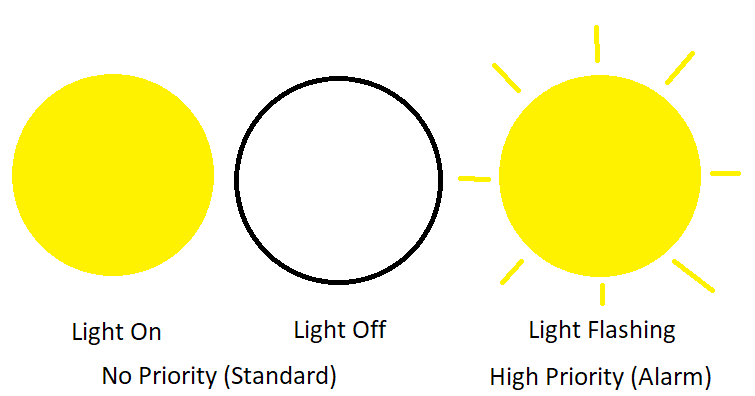
\includegraphics[width=0.4\textwidth]{AlarmPriority.png}
\caption{ \space Potential lighting states based on priority.}
\label{Alarm Priorities}
\end{figure}
\subsection{Application Layer (Linux Base-to-Base Emulation)}
Our intentions in creating the Linux base-to-base emulation of our system was due to not having access to the hardware in a timely fashion.  The application layer was divided into different files for simplicity and organizational purposes.  It emulates the menu items displayed on the screen (as would be seen by a user) and it emulates a network in which a device is connected.  This Linux version of the system simulates sending a help packet to the contacts listed in a user’s friends list.  A packet will be sent to the first contact on the list, it will timeout if the help request is not acknowledged as received, at which time it will be sent to the next contact on the list.
\subsection{Button to Base Application}
The button-to-base station communication is programmed using the General Access Profile (GAP) layer and the Generic Attribute Profile (GATT) layer of Bluetooth Low Energy.  Accessing the API’s listed in bluenrg1\_api.h allows for the utilization of advertising packets over the air according to Bluetooth standards.  The GAP layer defines the basic requirement of a Bluetooth device.  It describes the device's role, its different modes, and its procedures for its mode to enable a connection between Master and Slave devices.  Once the GAP has been initialized with its role as a peripheral, its mode is set to be connectible to any device or in Generally Discoverable mode and its procedure to this mode is to establish a connection to any device that tries to connect to it then it could continue establishing security parameters for pairing. The ADV\_IND flag is used for General Discovery mode. The justification behind the General Discovery mode and its respective procedure is that in case the advertising button is lost or damaged the user could easily reestablish connection with the new advertising button with no technical help. When not advertising the BlueNRG-1 is then listening for a connection response from the initiator, the Master device. Once connected the Slave device sends a slave security request to the SAMB11, which then the Security Manager handles any pairing transactions. Before any connection takes place the scanning device, the SAMB11 must also be configured to be a central device.

The Atmel SAMB11’s GAP layer must also be initialized, which is accomplished using the API's listed in at\_ble\_api.h.  Its role is set as a central device with a General Discovery procedure. The General Discovery procedure allows the central device to scan the surrounding advertising devices. Again, this is so that in case the user loses or damages the advertising button the user could easily reconnect the new button to the central device. The AT\_BLE\_SCAN\_GEN\_DISCOVERY flag is used to scan all advertising Bluetooth devices. To guarantee that he central device only connects to the intended advertising button, the SAMB11 scans the local names of the advertising devices. As it scans if it finds the string "BlueNRG1\_Chat" it has successfully found the BlueNRG-1 advertising. This string can be changed on the BlueNRG-1 to another appropriate name. Once found the connection process is initiated by the SAMB11. If authentication and encryption is used then as the SAMB11 scans the BlueNRG-1's slave security request will come with the advertised payload of the packet sent.

The Security Manager authenticates the connection between the Master and Slave devices by exchanging the 128-bit Long-term-keys (LTK) generated by the AES algorithm. Unfortunately, because the advertising button does not have a display to enter a passkey, the encryption method used is the "Just Works" pairing method for both devices. This means that the connection is exposed to Man-In-The-Middle (MITM) attacks. An argument could be made that not much security is needed since all that would be transmitted between these two devices is "Help Request" packets and battery voltage levels. On the press of a button the BlueNRG-1 sends a connection request to the SAMB11. When the SAMB11 responds an exchange of LTKs are then exchanged to pair both devices together.  When both devices finish exchanging the LTKs, pairing is complete and the device's transition from the GAP layer to the GATT layer. When entering the GATT layer the roles implicitly change from Master\textbackslash Slave to Server\textbackslash Client.
The Server is the device that has updated data to send and the Client is the device that stores and processes this information. In this case the BlueNRG-1 is implicitly the Server and the SAMB11 is the Client. The BlueNRG-1 is the server because it has the voltage level that the base station needs to worry about and it is the device that sends the "Help Request" data the base station needs to process. Before the BlueNRG-1 enters the GATT layer it already has configured a table shown in Table \ref{BT Access}. 
\begin{table}[H]
\centering
\caption{Bluetooth Profile Table}
  \begin{tabular}{|l|c|c|c|c|}
      \hline
      Description         &Handle& UUID              & Value\\
      \hline
      Chat Service 	      & 0x0C & 0xD973F2E0...66   & \\
      \hline
      TX Characteristic   & 0x0D & 0xD973F2E1...66   & \\
      \hline
      Notif Handle	      & 0x0E & 				     & uint8*\\
      \hline
      CCCD                & 0x0F & 			         & \{0, 1\}\\
      \hline
      RX Characteristic   & 0x10 & 0xD973F2E2...66   & \\
      \hline
      Write Handle		  & 0x11 &					 & uint8*\\
      \hline
      Battery 		      &		 &					 & \\
      Characteristic	  & 0x12 & 0xD973F2E3...66   & \\
      \hline
      Read Handle		  & 0x13 & 					 & uint8*\\
      \hline
  \end{tabular}
  \label{BT Access}
\end{table}
A Bluetooth Profile may consist of the many services, characteristics, and attributes. In the profile created for the button to base communication only one service is created that contains three characteristics.  The handles give order to the table in organization of service, characteristic, and attribute order. Each characteristic has a description of itself and it identifies itself through the UUID. The UUIDs in the button to base profile are all custom characteristics therefore, they all must be 128-bits.  Generic characteristics are 16-bits. Each characteristic must also have a property that gives both devices the ability to send and receive data that modifies their respective attribute values.
\begin{figure}[H] 	% There are several different modifiers that can be used in [].
\centering
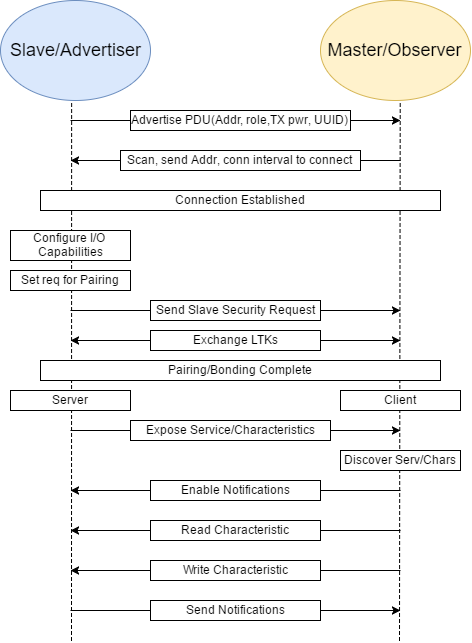
\includegraphics[width=0.4\textwidth]{Bluetooth.png}
\caption{ \space Bluetooth LE sequence of events}
\label{ble}
\end{figure}

Now in the GATT layer, to be able to chat back and forth between the BlueNRG-1 and SAMB11 the "TX Characteristic" and "RX Characteristic" were made. These are just names of course to what actually allows the transactions of data to take place. The BlueNRG-1 exposes the characteristics shown in Table 8. The SAMB11 then goes through the discovery process of these characteristics. Once discovered, both devices have the same characteristics with the same handles stored. The SAMB11 will discover that the TX characteristic contains the Client Characteristic Configuration Descriptor (CCCD) that comes when the notification property is initiated by the Server. The CCCD attribute value will only take a 0 or 1. The Client will write a 1 to the Server to enable Notifications from the Server. Writing a value of 0 disables Notifications from the Server. When the Client enables Notifications the Server will now be able to send data to the Client through its attribute handle without the need for acknowledgement from the Client. The Client will discover the RX Characteristic, which comes with the Write Property, the handle, and the attribute value. Once discovered the Client would then be able to write to this handle and the Server would then receive the data sent. Lastly, the Client discovers the "Battery Characteristic" along with its Read Property, its handle, and attribute value. The Client could now on command inquire to the Server for some information designated by the Server. In this projects case it would be the battery voltage level being inquired about. Fig. \ref{ble} will help with the visualization of the sequence of events between the Master\textbackslash Slave and the Server\textbackslash Client.

Another concern was the power consumption of both the BlueNRG-1 and the SAMB11. To alleviate the radio from being constantly ON. The BlueNRG-1 would be put into sleep mode and wake up every 10 seconds so as not to go into Deep Sleep. In this application the BlueNRG-1 would consume less than 1 $\mu$A and while connected it would consume almost 5 mA. To alleviate the power consumption of the SAMB11 scanning, it would be best to reduce the scanning window. The SAMB11 would be scanning half the time ON and the other time OFF in the interval of 30 ms. It was found that in this application it would consume about 3 mA. The drawback to reducing the scanning window of the SAMB11 is that it may take longer for the BlueNRG-1 to connect to it when waking up and then sending its advertisement to connect.

\subsection{Button Hardware}

The button is the main user-end device of this HA-HA project. It was designed with emphases on maximizing battery life, "wearability", user-friendliness, and reliability.  The button itself is a device that is less than 1.3" x 1.5" x 0.3" in physical size (without packaging). The physical size of the bilayer PCB is as small as is possible for the design, as in most wearable hardware devices.  The backside of this board holds each component with which an intended user may interact, including a tactile switch\footnote{ The "Button" portion of the "HA-HA Button"}, two low-energy LED indicators, and a 20mm coin cell battery holder. The top side of the board hosts a microcontroller, 2.4GHz antenna, and SWD connectors.

\subsubsection{User Interface}

\begin{figure}[H]
\centering
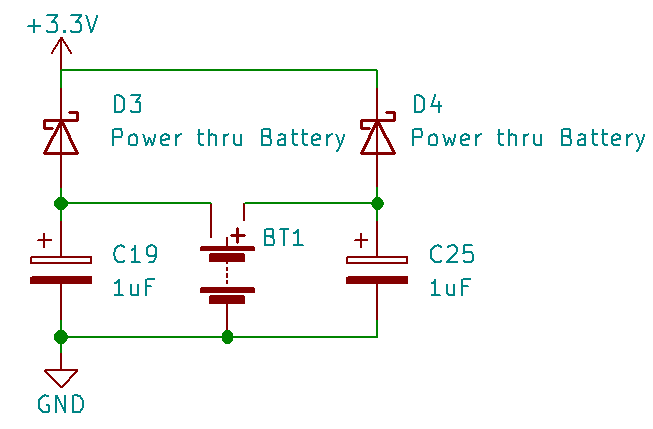
\includegraphics[width=0.3\textwidth]{buttbat.PNG}
\caption{Button Schematic: Coin Cell Battery Holder}
\label{buttbatt}
\end{figure}

By using standard CR2032 coin cell batteries, the button both maintains a small form factor and can potentially allow for easier maintenance by users.  The choice of battery holder was influenced by its small form factor and its intuitive design for replacing batteries that is very user friendly. However, by allowing users to replace their own batteries, a designer must consider an incident in which a user accidentally inserts a battery in reverse polarity.  To prepare for such an event (or any other instance of reverse polarity charge flow), Schottky diodes are added in series between each positive terminal of the the battery holder and the device's voltage rail, as can be viewed in Figure \ref{buttbatt}. One may also note the pair of 1$\mu$F capacitors in Figure \ref{buttbatt} placed about the battery holder. These are used to maximize the life of the coin cell by providing low-internal-resistance sources of energy to the other components of the button during current spikes.

\begin{figure}[H]
\centering
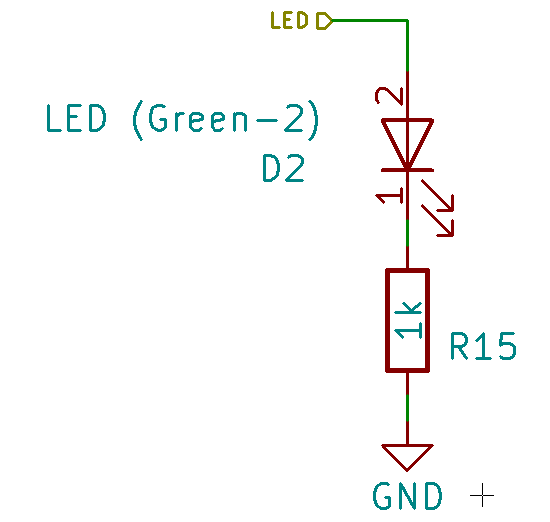
\includegraphics[width=0.2\textwidth]{buttled.PNG}
\caption{Button Schematic: LED Indicator}
\label{buttled}
\end{figure}

The basic LED indicator circuit implemented on the button is given in Figure \ref{buttled}. The LED expends a mere 2mW of power during normal (forward) operation. Because the LED can be driven by 1mA of forward current, it was possible to connect the LED directly to a microcontroller GPIO\footnote{Max current that can be sourced by a GPIO pin on the BlueNRG-1 = 17.6mA.}.  This LED will blink when a neighbor has responded to a user's distress signal.

\begin{figure}[H]
\centering
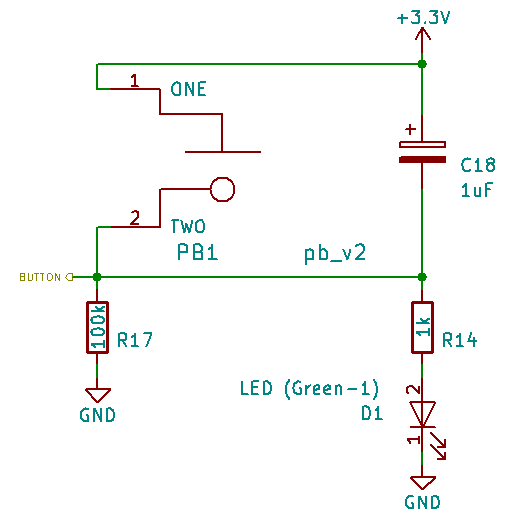
\includegraphics[width=0.2\textwidth]{buttbutt.PNG}
\caption{Button Schematic: Button}
\label{buttbutt}
\end{figure}

Figure \ref{buttbutt}~displays the basic design of the device's button, which is connected through its lower terminal to a GPIO of a microcontroller. When the button is unpressed, the microcontroller will read no voltage, and when the button is pressed, [almost] the entirety of the current will flow through R14 shown. An LED, similar to that used by the LED indicator, has been added to allow for users to easily confirm their button push. In the future, this button may be without this LED, and instead its press will signal to digital logic to drive the LED circuit once more in Figure \ref{buttled}.

\subsubsection{Design Using the BlueNRG-1}

\begin{figure}[H]
\centering
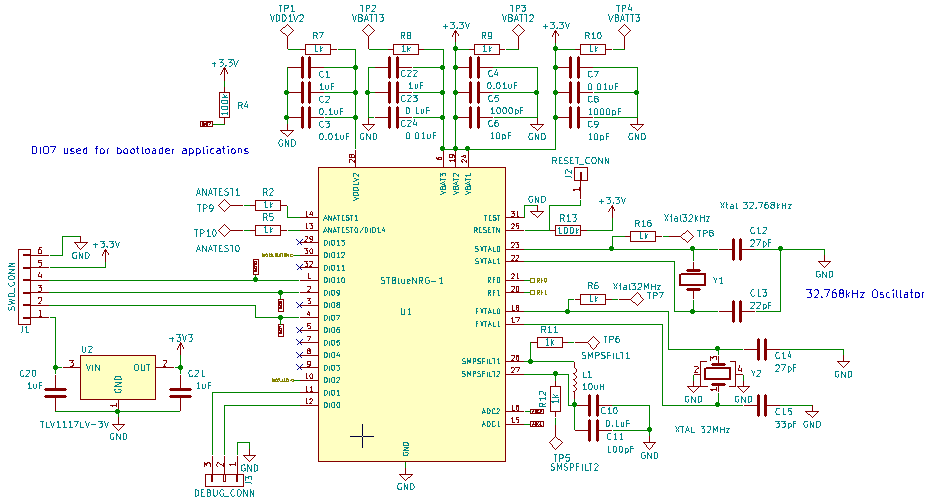
\includegraphics[width=0.4\textwidth]{buttmcu.PNG}
\caption{Button Schematic: BlueNRG-1 Microcontroller}
\label{buttuc}
\end{figure}

The BlueNRG-1 microcontroller was selected for use in the button due largely to its extremely low-power operation and its integrated Bluetooth LE module.  This microcontroller is the brains of the button, and has only one main function: it is responsible for translating a button press into a distress signal that is transmit over Bluetooth to its paired base station, which further forwards that signal.

The BlueNRG-1 runs two external crystal oscillators: a 16MHz or 32MHz fast clock for RF applications and a 32.768kHz clock for low-power operation. The microcontroller also implements a DC-DC converter that outputs 1.4V. Each of these components require careful planning during layout, but are relatively simple to properly implement during initial design.  The values of the capacitors must, in series, match the load capacitance of their accompanied crystals.  To properly implement the integrated DC-DC converter, one must use a large inductor (in this case 10$\mu$H) with a very low DC resistance (<1$\Omega$) and rated for high currents (>100mA).  All capacitors used were C0G due to their low loss.

\begin{figure}[H]
\centering
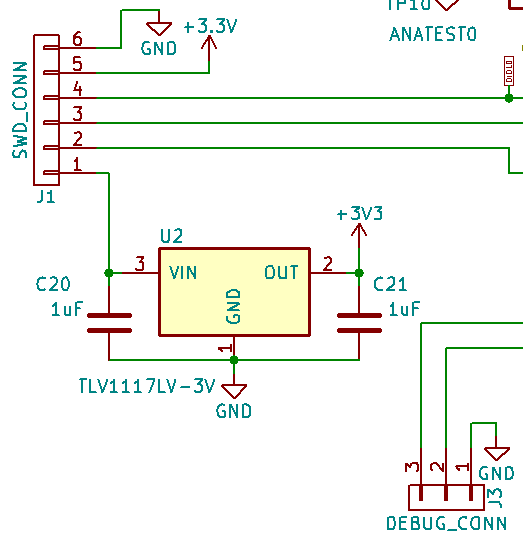
\includegraphics[width=0.3\textwidth]{buttswd.PNG}
\caption{Button Schematic: BlueNRG-1 SWD Interface}
\label{buttswd}
\end{figure}

Since the project will be carried on and made open source, it is important that the button can be reprogrammed.  To be able to program the BlueNRG-1, proper SWD connections must be made.  Aside from the mandatory SWD pins\footnote{Namely: VREF, SWDIO, SWDCLK, RESET, and GND} for programming the device, pins DIO0 and DIO1 were routed to connections to allow for the transmission of more detailed debugging information. ST also recommends that DIO7 is pulled high during debugging to load a factory-installed bootloader.

\subsubsection{Button Layout}

\begin{figure}[H]
\centering
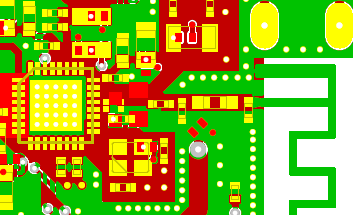
\includegraphics[width=0.4\textwidth]{button_ship_nice.PNG}
\caption{Button Layout}
\label{buttlay}
\end{figure}

Figure \ref{buttlay}~displays the microcontroller, 2.4GHz MIFA with $\pi$ matching network, 16MHz crystal oscillator, and 32.768kHz oscillator in one image. One must go to great lengths to attempt to isolate the ground planes of the microcontroller and oscillators from the noisy RF ground plane.  One method proposed by the BlueNRG datasheet involved using low Q inductors between the capacitors used in each oscillator and the ground plane.

Test points were very useful for testing the board. These point were connected in series to points of interest by large resistors.

\subsubsection{Results and Future Work}

By the end of the project, the button is still inoperable. It is believed that two weeks of testing were lost testing burnt microcontrollers on badly butchered boards, and more recently limited successes have been achieved.  A recent board that was soldered by 'skilleting' the PCB using solder paste maintained stable and accurate voltage rails, almost indefinitely.  However, while further testing on the board was conducted in an attempt to explain the absence of signal being generated by the crystal oscillators, the current drawn by the board very slowly increased from 2mA to roughly 45mA before the board simple "shut off", or altogether stopped drawing current. After this event, the board continued to work intermittently while more testing was carried out in an attempt to explain the previous behavior. It was noted that both the 1.2V LDO output digital rail and the 1.4V DC-DC switching regulator output became less and less stable as this current approached 45mA, before the board again seemed to reset. After this 'reset', all regulators stopped working for a time. 

\begin{figure}[H]
\centering
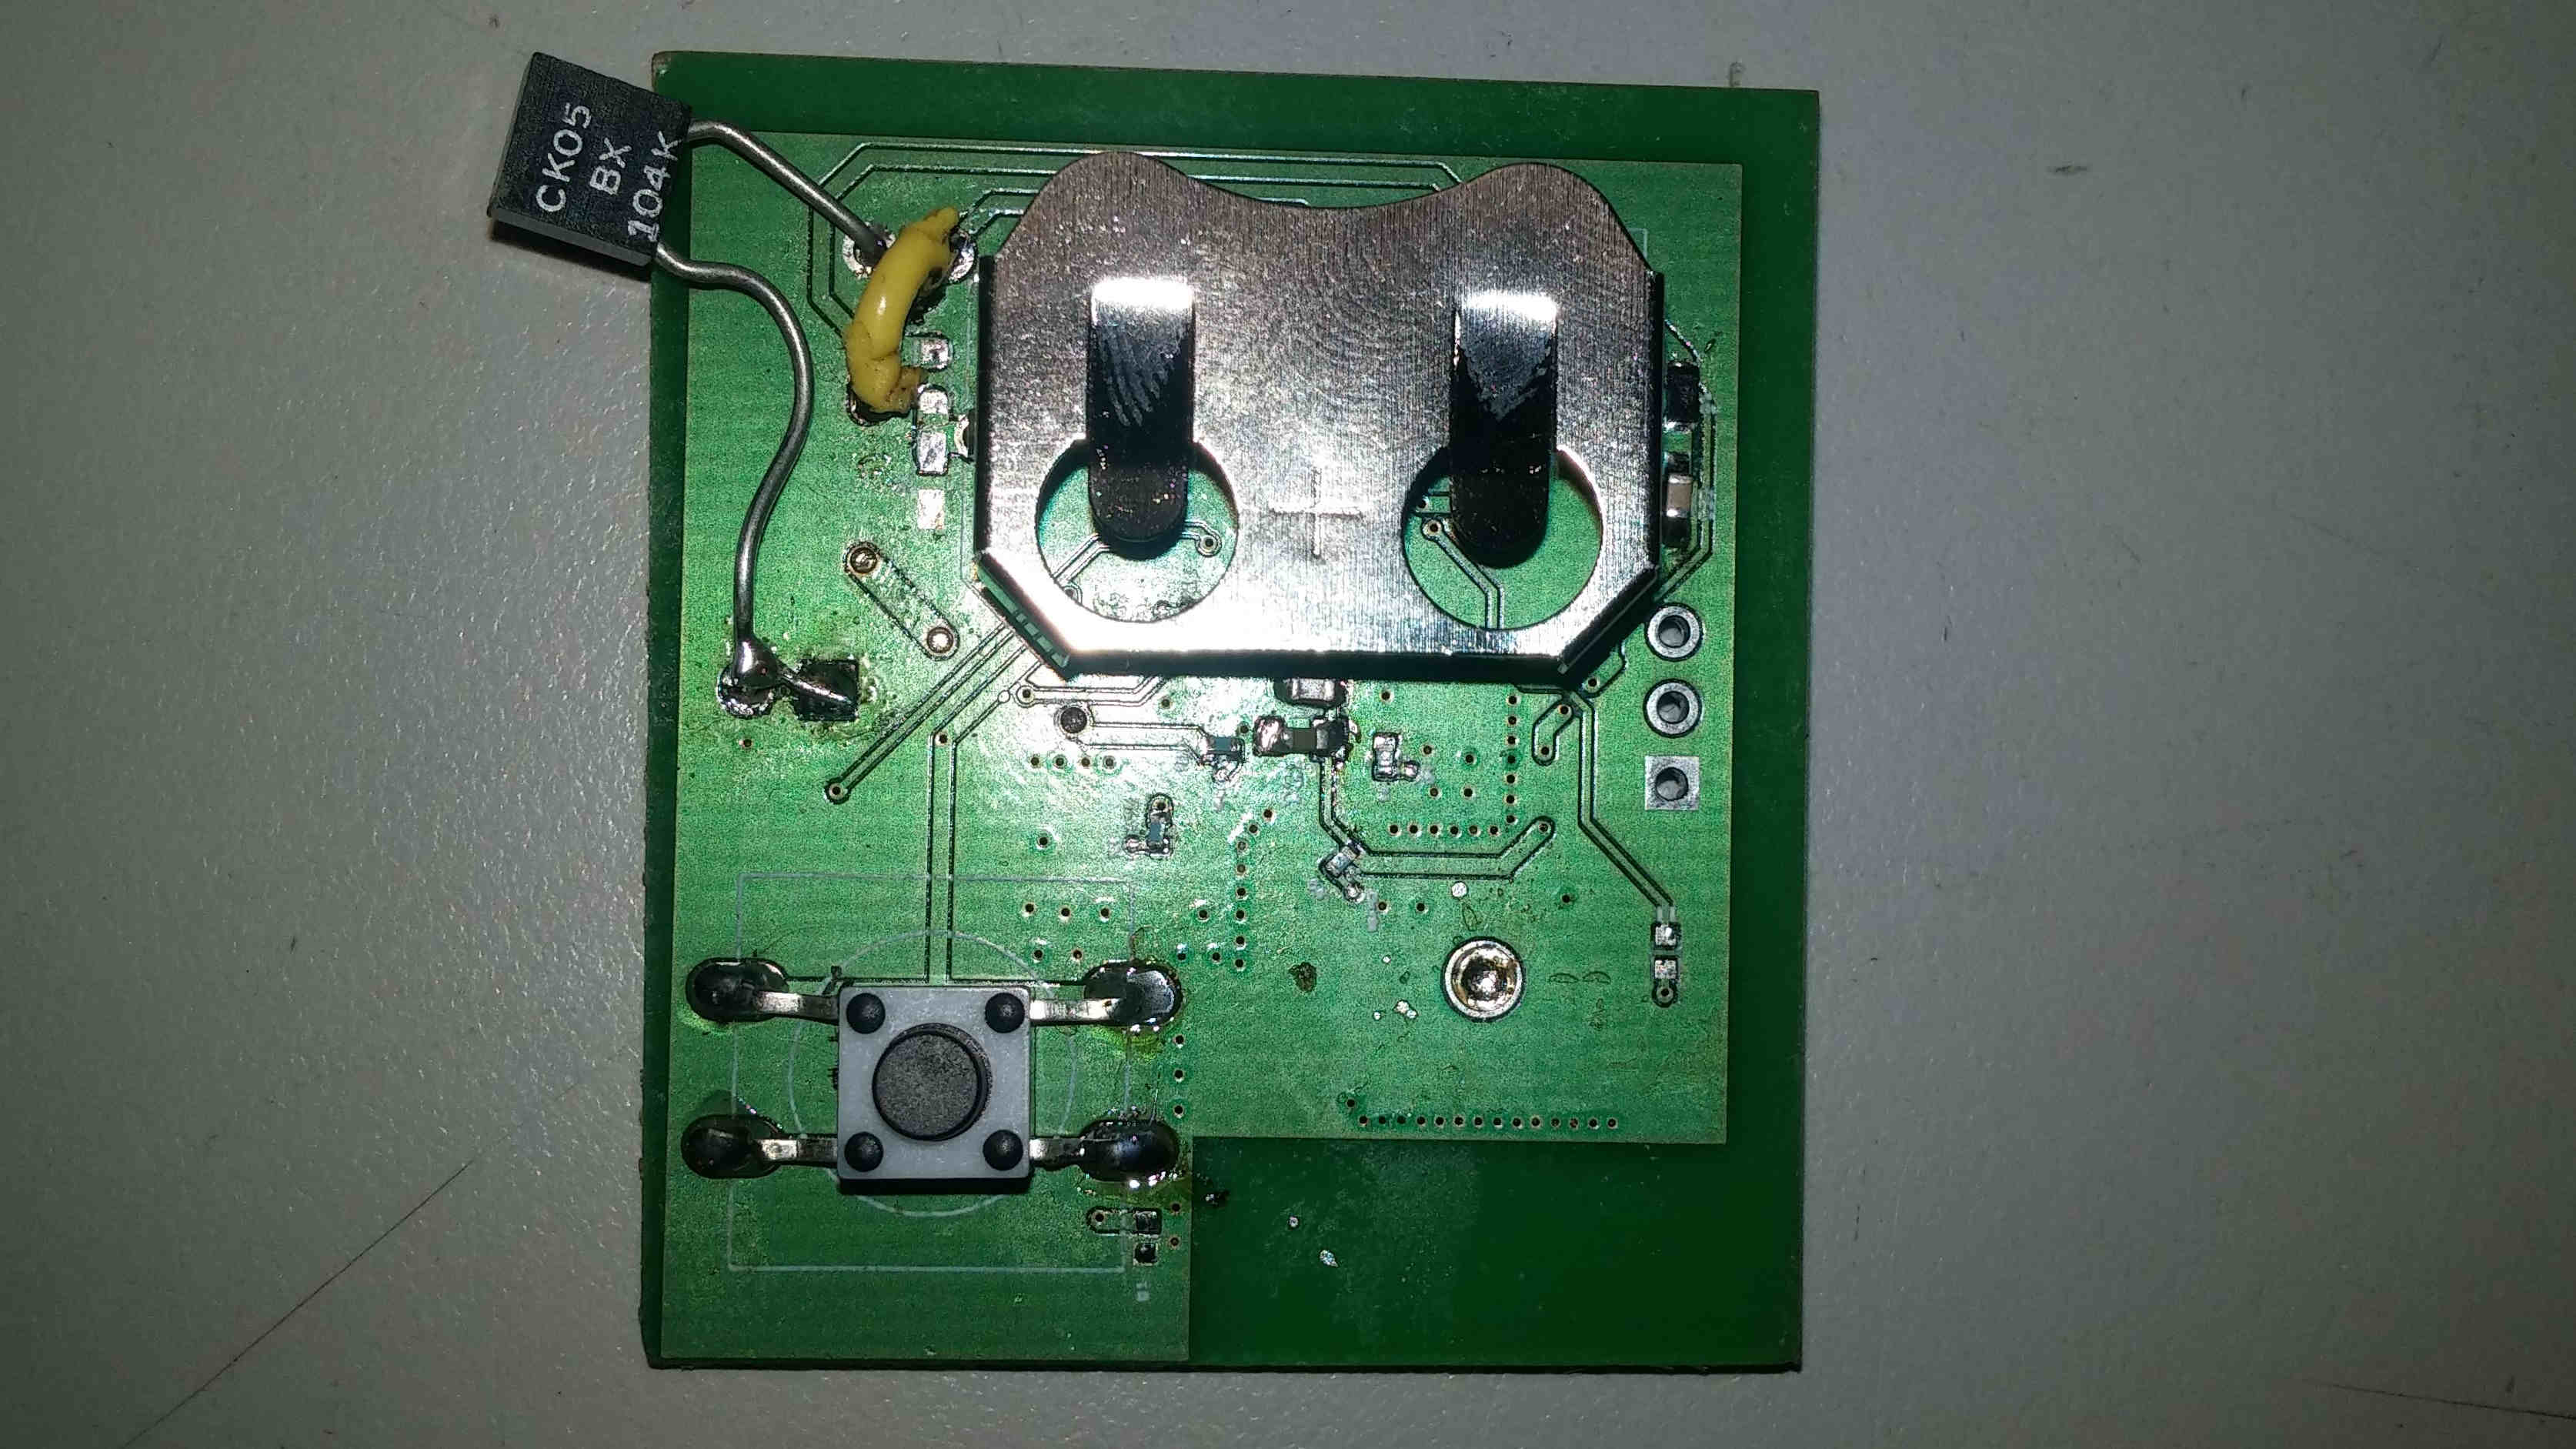
\includegraphics[width=0.4\textwidth]{moose2.jpg}
\caption{Semi-Functional Test Board}
\label{butttest}
\end{figure}

\subsection{Base Station Hardware}

\subsubsection{Schematic}

The base station unit is the other crucial component to this decentralized ad hoc neighbor system. Each household contains a single base station unit that pairs with its own unique button. When the button signals a help request, the corresponding base station receives the signal and broadcasts the help request to nearby friendly base stations in search of a response. The help signal is recursively rebroadcasted by the receiving base stations to any immediate base stations within their broadcast range, allowing for a theoretical unlimited search range. This work-around allows the system to get past the limited radiation power set under the FCC Part 15 regulations for unlicensed low-power transmitters.

The base station consists of a bottom-up stack of PCBs. The bottom board contains the power supply, battery backup, as well as the amplifier and switching circuit for the speaker and light. The microcontroller sits on the board just above with both the 2.4GHz and 900MHz antennas. Female pin headers are extended from this board to allow placement of 16x4 character LCD display PCB just above.

\begin{figure}[ht] 	% There are several different modifiers that can be used in [].
\centering
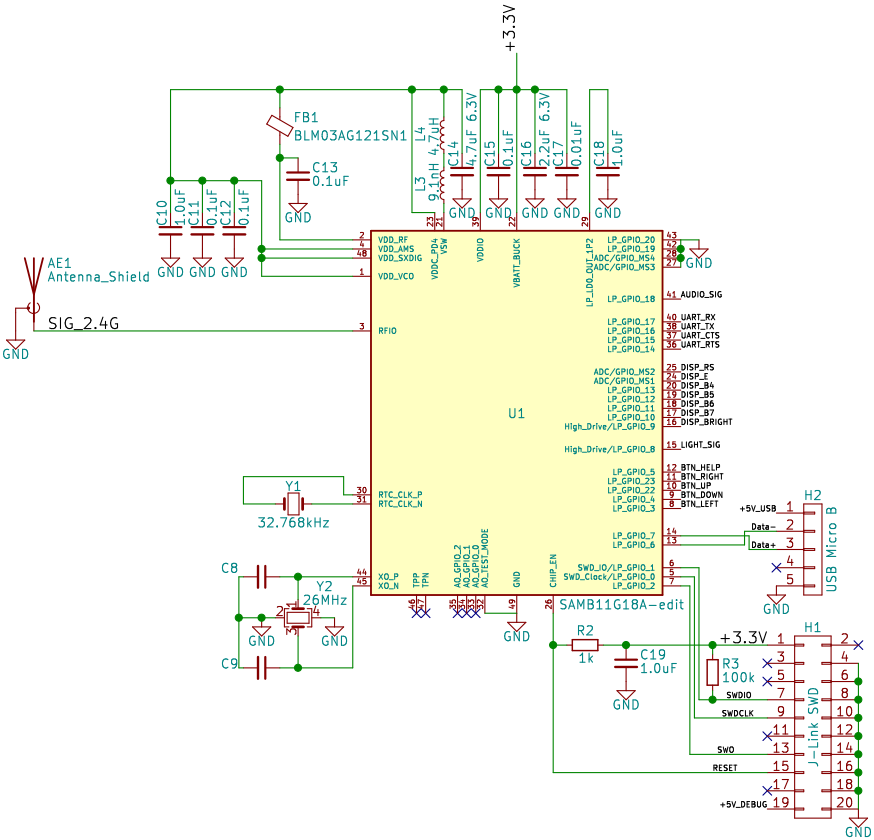
\includegraphics[width=0.4\textwidth]{base-schematic-uc.png}
\caption{ \space Base Station Schematic: Microcontroller}
\label{base-sch-uc}
\end{figure}

The Atmel SAMB11 system-on-chip is the base station's microcontroller. It features a quad-flat-no-lead (QFN) packaging with 48 pins and a pitch of 0.4mm distance between pins on a single side. The microcontroller provides an on-chip Bluetooth Low Energy module that allows easy access to the 2.4GHz radio band. The microcontroller operates with two external crystal oscillators: a 32.768kHz real time clock and a 26MHz normal operation clock. The SAMB11 operates on a +3.3V voltage rail for its digital core, but it also contains an internal DC-DC converter to +1.2V for radio operations.

The microcontroller has a total of 27 GPIO pins, where 4 pins have mixed-signal capabilites and the rest are standard digital. The SAMB11 has an on-board analog-to-digital converter (ADC) accessible by these mixed-signal GPIOS, but our system does not have use of this. Instead, these GPIOs are used as typical digital pins. All on-board GPIOs have internal resistors, whose pull orientation can be programmed.

The on-board Bluetooth module is accessed via the RFIO pin, which handles both the receiving and transmitting radio ends. Our system provides a patch antenna tuned to 2.4GHz operation with a matching network of transmission lines. Unlike the button, the base station is not limited to be as small as possible. Therefore, instead of using a more compact, electrically-short chip antenna that has limited performance, the system takes advantage of the extra real estate with a higher-performance patch antenna.

The controller is programmed via serial wire debug (SWD), which requires 5 signals for operation: voltage reference, IO, clock, reset, and ground. The IO and clock is connected directly to the corresponding pins on the microcontroller, while the reference voltage and ground is connected to the digital core voltage of +3.3V and the microcontroller ground, respectively. The SWD reset pin connects to the microcontroller's CHIP\_EN, which is required to stay high for normal operations. The debugger momentarily pulls CHIP\_EN low to restart the system. While the GPIOs have internal pull up/down resistors, an external pull up resistor must be placed by CHIP\_EN to ensure an operational chip in the absence of the SWD debugger.

\begin{figure}[ht] 	% There are several different modifiers that can be used in [].
\centering
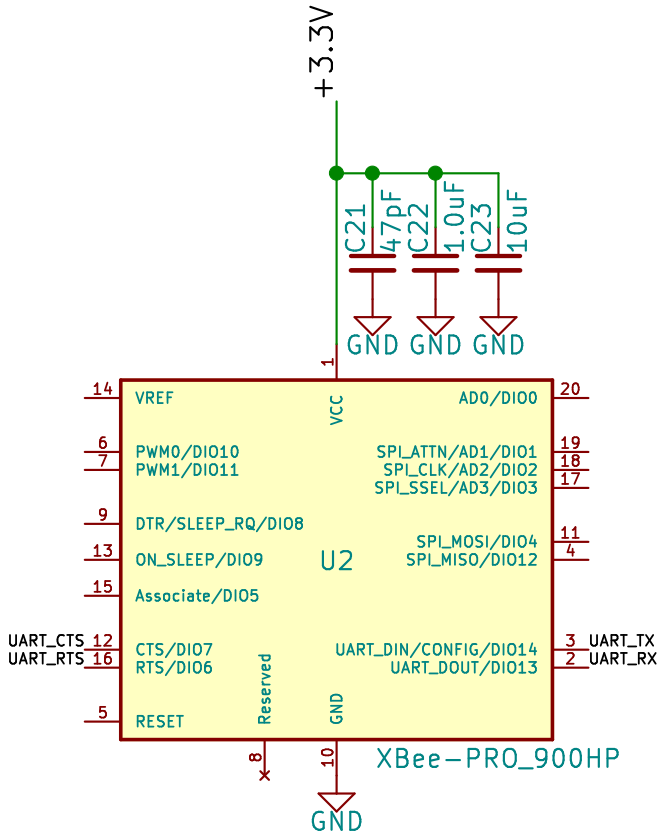
\includegraphics[width=0.4\textwidth]{base-schematic-xbee.png}
\caption{ \space Base Station Schematic: XBee Transceiver}
\label{base-sch-xbee}
\end{figure}

The Digi XBee radio module is the choice of transceiver to communicate on the 900MHz band. An external antenna can be connected through its on-board SMA connector and on-board PCB can also be integrated or mounted onto the circuit with minimal dimensional impact. The XBee communicates with the microcontroller via UART with 4 pins: receiving data (RX), transmitting data (TX), clear-to-send (CTS), and request-to-send (RTS).

\begin{figure}[ht] 	% There are several different modifiers that can be used in [].
\centering
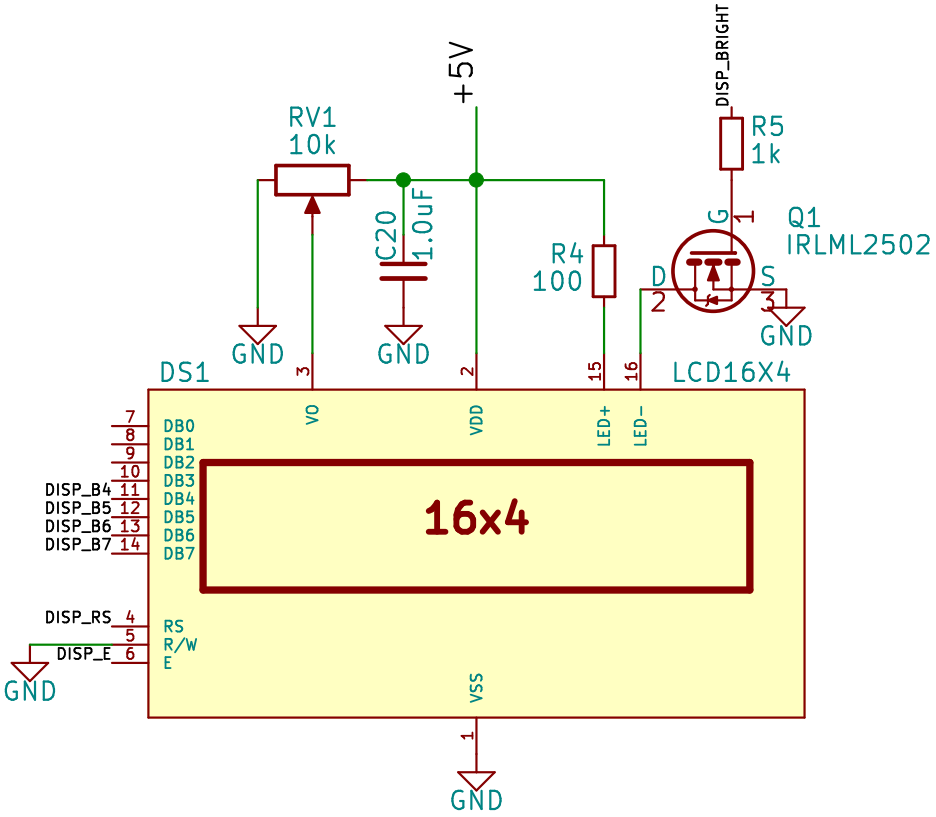
\includegraphics[width=0.4\textwidth]{base-schematic-lcd.png}
\caption{ \space Base Station Schematic: Display}
\label{base-sch-lcd}
\end{figure}

A 16x4 character LCD display is chosen for user interface to the base station system. It provides a larger space for viewable data than its 16x2 character counterpart, while remaining relatively inexpensive in comparison to other larger display screens. The LCD is the only device on the board that operates on a +5V rail as opposed the microcontroller's +3.3V rail. The register select (RS), read/write, and enable pins control the data flow set by the 8 data pins of the LCD. To conserve on limited GPIO resource, the LCD was set to half-byte operation, reducing the necessary data pins down to 4. The ability to view the LCD depends on its character contrast and the backlight brightness. A trim-pot resistor allows for contrast tuning based on the user's viewing angle, while the LCD backlight is controlled via a PWM signal from the the microcontroller to a power MOSFET.

\subsubsection{Layout}

\begin{figure}[ht] 	% There are several different modifiers that can be used in [].
\centering
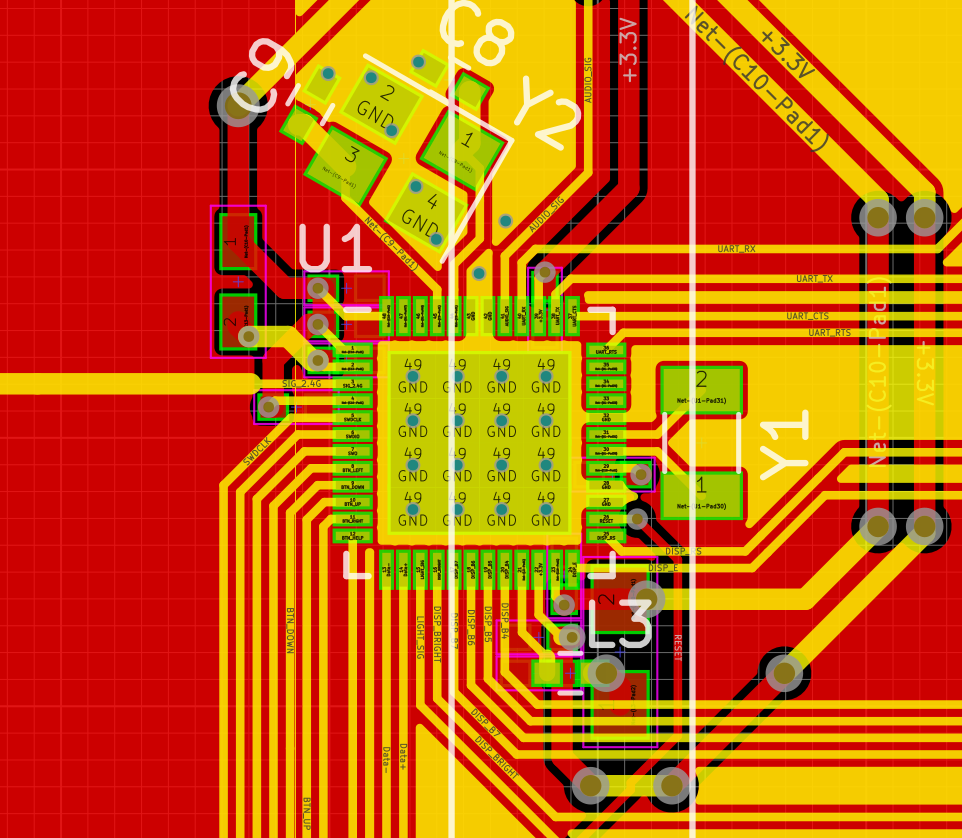
\includegraphics[width=0.4\textwidth]{base-layout-uc.PNG}
\caption{ \space Base Station Layout: Microcontroller}
\label{base-lay-uc}
\end{figure}

Layout of the microcontroller on the base station demands careful consideration due to the tiny nature of the chosen components, which are sized in the sub-centimeter range. The biggest concern is the noisy nature of any electromagnetic interference (EMI). This interference can be found everywhere, but on a PCB, the main sources can be found in crystal oscillators, power supplies, and antennas. The high frequency components found within these elements is the origin to this noisy behavior.

As such, crystal placement is of utmost importance. While the crystal can inflict noise onto nearby signal traces, the oscillator itself is also very prone to noise. The microcontroller requires a clean oscillating signal to operate properly with its clocking signal. Placing the crystals as close as possible to the microcontroller allows for short connecting traces and reduces the possibility of defect in the oscillating signal. In addition, the 26MHz crystal has a ground pad, which must have a low impedance short return path to the microcontroller. By low impedance, we mean a minimally-disrupted wide path that allows current to flow relatively freely. This low impedance short path reduces the ground loop in which current flows, lowering the noisy effect on nearby traces. To further reduce any noise coupling, signal traces should avoid as best as possible the immediate vicinity of the crystals.

The analog signal through RFIO is the Bluetooth data signal that is handled by our on-board patch antenna. The feedline trace for the antenna is relatively isolated from any components in the same reason traces avoid areas near the crystals. Nearby components will always carry some sort of EMI from the stray capacitance and inductance. This semi-isolation tactic reduces the chance of noise but also creates a clean analog ground return to the microcontroller.

\begin{figure}[ht] 	% There are several different modifiers that can be used in [].
\centering
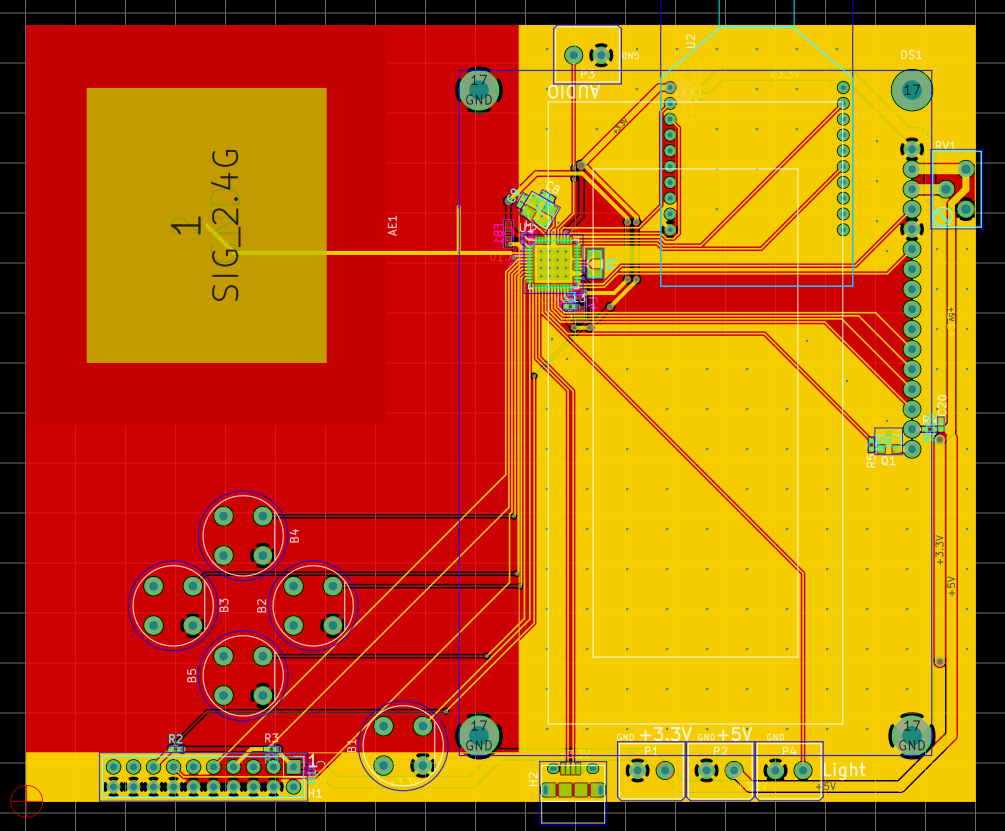
\includegraphics[width=0.4\textwidth]{base-layout-full.PNG}
\caption{ \space Base Station Layout: Radio and Display}
\label{base-lay-full}
\end{figure}

Because the base station operates on two different frequency bands, the 2.4GHz and the 900MHz, the layout must include sections for the antennas. Placement of these elements should be as far away as possible to avoid any unnecessary couplilng, as antenna behavior is heavily affected by its surroundings. The patch antenna is used for broadcasts in the 2.4GHz domain, and it has a shorted transmission line stub to match the input impedance of the microcontroller's RF end with the antenna's characteristic impedance. On the other side, the Digi XBee module is used for broadcasts in the 900MHz range. The XBee takes digital UART signals from the microcontroller before passing through its own onboard gain and modulation stage for the mesh network signals. As a result, we do not have to strictly follow the same analog isolation rules as the 2.4GHz signal. The XBee has an SMA connector which allows us to place an external antenna on the device, however, these tend to be more expensive and difficult to reproduce. Three excellent in-house designs were created which perform very well, are more compact, and also more configurable to a variety of different geometric dimensions, making them a less expensive and more sustainable antenna for the base station.

The 16x4 LCD display is connected via 16 pin headers. placing the same 16 pin headers in female form so the required land space for placement is reduced by instead stacking the LCD right above the XBee module. The extra female headers provide the air space needed to avoid any component collision. The LCD also has 4 large mounting drill holes, which will double up and make use of as the common ground connection between the LCD, the microcontroller PCB, and the power supply PCB.

Because of the large ground planes on both the top and bottom sides of the PCB, stitching vias are scattered around the board. This connects the two ground planes together and ensures the ground potential through out the board is relatively the same. Additionally, these vias provide extra paths for ground currents to flow back to their original source.

\begin{figure}[ht] 	% There are several different modifiers that can be used in [].
\centering
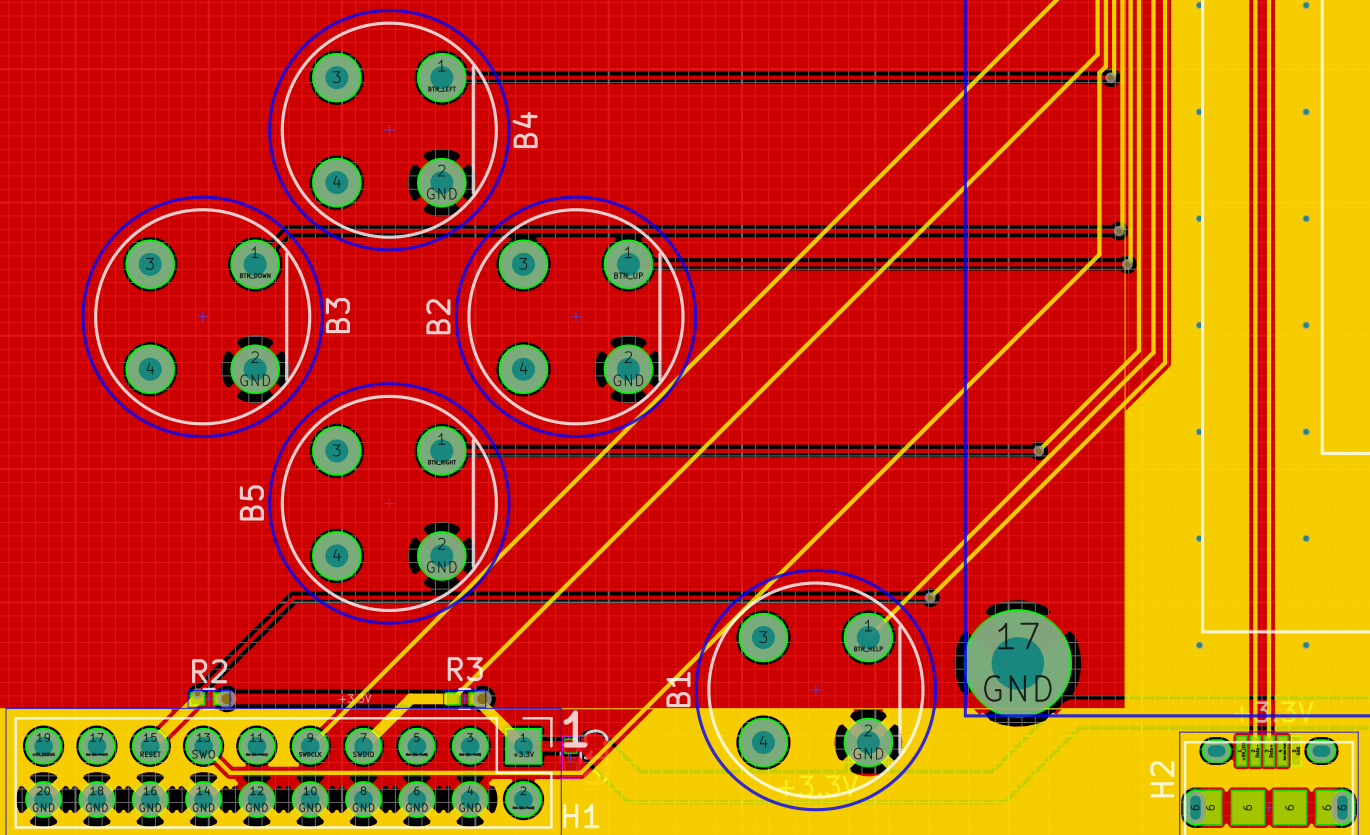
\includegraphics[width=0.4\textwidth]{base-layout-interface.PNG}
\caption{ \space Base Station Layout: Interface}
\label{base-lay-btn}
\end{figure}

In addition to the LCD, user interface is additionally provided through a 20 pin SWD connection and a micro USB B receptacle. The SWD IO and clock are connected directly to the microcontroller's SWDIO and SWDCLK, SWD reset is connected to CHIP\_EN, and the voltage reference and ground and connected to +3.3V and the PCB ground respectively. Because these signals do not change in voltage necessarily at the same time, it is best to place them as far apart as possible. This prevents nearby inductance from signal traces to inflict faulty digital highs/lows between one another. In contrast, the USB micro has a pair of differential data pins. Traces to these pins should be closely coupled with equal trace lengths. All other unrelated trace signals should avoid the area to avoid disrupting this differential pair signaling.

\subsection {Power Supply \& Peripherals}

\begin{figure}[ht] 	% There are several different modifiers that can be used in [].
\centering
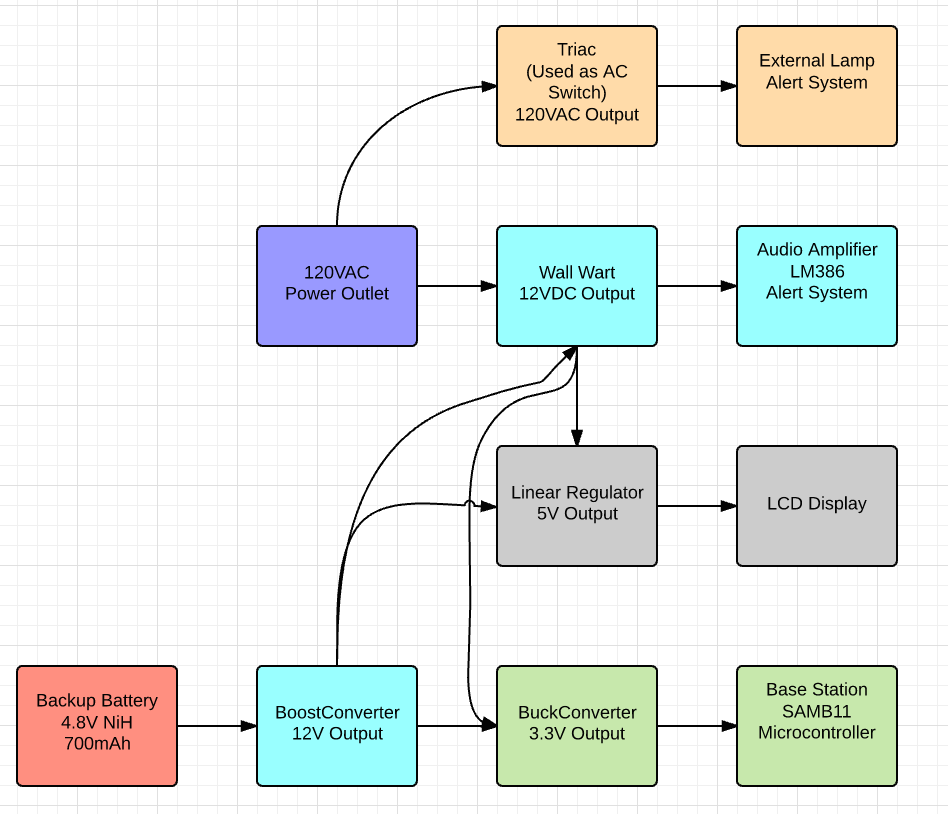
\includegraphics[width=0.4\textwidth]{BlockDiagram.png}
\caption{ \space Power Supply \& Peripherals Block Diagram}
\label{Psupply}
\end{figure}

\subsubsection{Power Supply}

The power supply for the base station requires three different output voltages to power the main components. The three output voltages are 12V, 5V, and 3.3V as we can see from the base station power budget. The base station pulls a maximum current of 394.6mA, and a maximum power of 1.82W. The high-level block diagram below illustrates the whole design of the power supply and peripherals. First of all, the base station is powered by a regular 120VAC power outlet that can be found in any home with electricity. A 12V 12W AC/DC external wall mount adapter from Qualtek is used to convert 120VAC to 12VDC. The 12V output from the wall mount adapter is fed to an audio amplifier circuit using a LM368 IC. The output from the wall mount adapter is stepped down to 5V using a linear voltage regulator. The 5V output from the linear regulator is fed to the LCD display as shown in the block diagram. Additionally, the 12V output is stepped down to 3.3V using a Buck Converter to feed the SAMB11 microcontroller, the X-bee pro, and the keypad. 

The power supply also has a 120VAC output that is controlled using a triac. The purpose of the triac is to let us change the output from 120VAC to 0V at any given time. The backup power consists of a 4.8V 700mAh NiMH rechargeable battery. A boost converter is used to step up the 4.8V from the battery to 12V. This allow us to feed 12V to the system like the wall mount adapter so that we can repeat the whole process to power the components in backup battery mode.

\subsubsection{12-Volt Output: Audio Amplifier}

\begin{figure}[ht]	% There are several different modifiers that can be used in [].
\centering
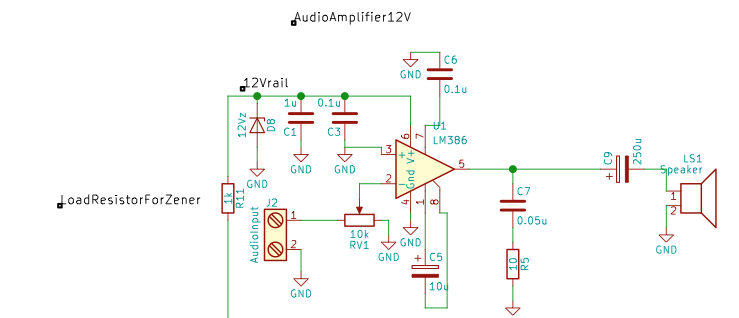
\includegraphics[width=0.4\textwidth]{Audio.png}
\caption{ 12V Audio Amplifier}
\label{Paudio}
\end{figure}

The 12V output from the wall mount adapter is fed to a LM386 audio amplifier as shown in the circuit diagram above. This means that the output audio signal can swing from 0V to 12V. A 12-Volt Zener diode (D8) is used as a voltage reference to make sure the input voltage rail does not exceed 12V, since it can damage the LM386 IC. However, a 1k$\Omega$ (R11) resistor was added to act as a load in case that the rail exceeds 12V to limit the current looping through the Zener diode. The input signal for the audio amplifier is regulated with a potentiometer using a voltage divider. In this case the gain of the amplifier was set to 200, which is the maximum gain possible. The gain can be reduced by adding a resistor in series with the 10uF capacitor (C5) between pin 1 and 8. Lastly, the output signal goes through a DC coupling capacitor to get rid of any DC components. 

\subsubsection {5-Volt Output: LCD Display}

\begin{figure}[ht]	% There are several different modifiers that can be used in [].
\centering
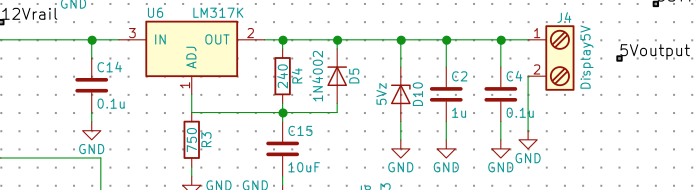
\includegraphics[width=0.4\textwidth]{Linear.png}
\caption{ 5V Output for LCD Display }
\label{Pdisplay}
\end{figure}

The LCD display requires a 5-volt input voltage and the data sheet suggests a 5-volt steady input signal to avoid any damages.  An adjustable LM317 linear regulator was used to step the voltage down to 5V.  The output of the linear regulator is given by Vout~= 1.25(1+R3/R4)V, the datasheet suggests keeping R4 at 240$\Omega$ but vary R3 to obtain the desired output voltage.  In this case, R3 is 750$\Omega$, which sets the output voltage to 5.15V.  The capacitor C15 is recommended to prevent any amplification of the output voltage ripple.  The Schottky diode D5 provides a low-impedance path for C15 to discharge so it won’t discharge at the output of the LM317.  A 5-volt Zener diode was included at the output of the LM317 to establish a voltage reference so it would not permit the output to exceed 5V in case of a malfunction.

\subsubsection {3.3-Volt Output: Microcontroller SAMB11, Keypad, and XBee-Pro}

\begin{figure}[ht]	% There are several different modifiers that can be used in [].
\centering
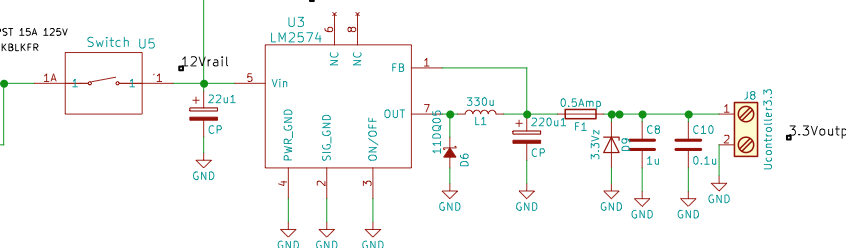
\includegraphics[width=0.4\textwidth]{Buck.png}
\caption{ Buck Converter 3.3V Output }
\label{PConverter}
\end{figure}

The microcontroller and the XBee-Pro are the most expensive and sensitive devices in the base station. For this reason, a 3.3-volt fixed buck converter LM2574 IC was used, instead of a standard adjustable buck converter.  The values of L1 and CP were chosen carefully so that the switching power supply is in continuous-conduction-mode.  A 3.3-volt Zener diode was added to set up a voltage reference at the output of the buck converter to double-protect the microcontroller and XBee module.  A 500mA fuse was included in case of any short circuits in either the microcontroller or the XBee.  A switch was then included before the input of the buck converter to control the three output voltages, which is not clear from the circuit diagram shown above.

\subsubsection{120VAC Output: External Light controlled with a Triac}

\begin{figure}[ht]	% There are several different modifiers that can be used in [].
\centering
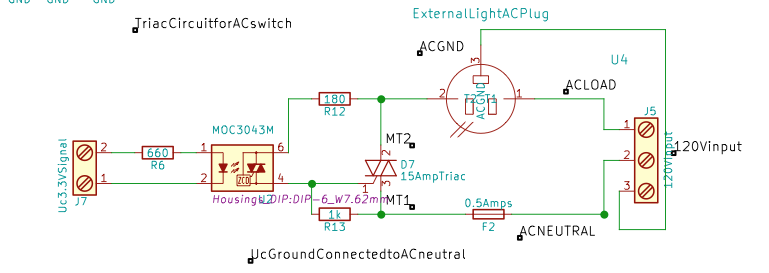
\includegraphics[width=0.4\textwidth]{Triac.png}
\caption{ 120VAC Output Controlled with a Triac}
\label{PTriac}
\end{figure}

The circuit in Fig. \ref{PTriac} allows the 120VAC output to change to 0V by sending a signal from the SAMB11 microcontroller.  The output is 120VAC when the microcontroller sends a high signal and 0V when the signal is low.  The triac blocks AC electricity when its gate senses no current.  To trigger the triac, the gate must sense a current of at least 25mA.  Unfortunately, the microcontroller could not output 25mA to trigger the gate.  To solve this, a MOC3043M optoisolator was included in the design, which can be activated with a minimum current of 5mA.  The optoisolator also completely isolates any AC currents from the microcontroller, which is essential, since AC currents and voltages can damage the microcontroller and the XBee-Pro.  The purpose of this circuit is to allow the user to plug any AC lamp into the base station to use as an alert, flashing in case of an emergency.  Note that this circuit will not operate in backup power mode.

\subsubsection{Backup Battery}

\begin{figure}[ht]	% There are several different modifiers that can be used in [].
\centering
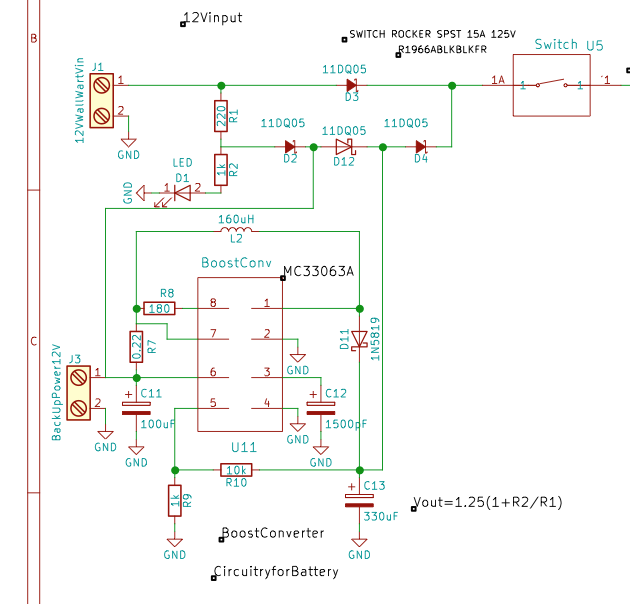
\includegraphics[width=0.4\textwidth]{Boost.png}
\caption{Backup Battery with Boost Converter}
\label{Pboost}
\end{figure}

The options for backup battery were limited by size, cost, capacity, and safety.  A 4.8V 700mAh NiMH battery met the criteria, however the output voltage of the battery is not compatible with the 12-volt main power rail.  A boost converter was used to step the voltage up from 4.8V to 12V.  This allowed the reuse of the wall-mount adapter step-down voltage process, which reduced complexity in the system.  The boost converter used is a MC33063A adjustable IC, the output voltage is given by Vout=1.25(1+R10/R9).  R9 was set to 1k$\Omega$ and R10 to 10k$\Omega$.  Thus, the output of the boost converter is 13.75V when the battery is fully charged.  However, the voltage of the battery drops when discharging so it is convenient that the output of the boost converter is greater than 12V much of the time during discharging.  The Schottky diodes D2, D12, and D4 are included to allow current flow in one direction to avoid any unwanted currents going to the boost converter or the battery.

\subsubsection{Future Revisions of Power Supply}

It was discovered with the final revision that output voltages were not at the required values.  For example, the output for the display was 3.7V instead of 5V, and the output of the boost converter is not 12V.  To correct this, different resistances must be tested experimentally until the desired output is achieved.  One of the primary concerns is a charging system design for the backup battery.  This charging system must be well designed to optimize the battery life and for the safety of the user, since batteries can be unstable at hot temperatures.  Finally, a noise filter must be designed for the audio amplifier because the output audio signal contains too much noise so static is audible without an audio input signal.

\subsection {Antenna Hardware}

The antennas were required to possess certain performance characteristics such as minimum link loss, a circular polarization, wide directivity, radiation pattern in all directions, and sufficient transmission range.  They also need to transmit and receive communications equally as well.

\subsubsection{Button}

The antenna for the button needed to operate in the chosen frequency band of 2.4 GHz and it was required to be compact so it can be contained within the button, which is to be worn as either a for a necklace or a bracelet pendant.  This size constraint required careful consideration to produce the optimum performance, which was a primary motivating factor to use this high-frequency band.  The minimum transmission range for the button is the approximate length of our customers’ homes at 50 feet and it must communicate with the base station in the home environment.  This means the button antenna needs to communicate through walls and despite other types of interference such as microwaves.

Several different 2.4 GHz PCB antenna layouts were initially designed based on proven engineering models, utilizing appnotes and datasheets as guides.  Subsequent revisions were created to properly tune the best performing antennas.  PCB antenna design requires careful consideration of the isolating ground plane, feedline dimensions, geometric configuration, keepout boundaries, and stitching vias, which are required to maintain proper radio-frequency (RF) potential.  These designs are comparatively simple but sensitive and complicated in practice.  Antenna testing is then a time consuming and meticulous process.

For lab testing, a high-frequency network analyzer was used to measure impedances with the baseline impedances measured first.  The SimSmith Smith chart simulation software was then used as a guide for designing impedance matching networks for optimum power transfer between the antennas and button circuit at the ideal impedance of 50$\Omega$ with no reactants.  An RF link was setup in the lab and a high-frequency spectrum analyzer was used to measure the far-field performance of each antenna.  The far-field is the region where the electromagnetic waves are free to radiate without the influence of the moving charges which produced them, once the waves have traveled far enough away from those charges.  In contrast, the reactive and radiating near-field regions are where these radiating waves are close to the charges and the current which created them.

\begin{figure}[ht]	% There are several different modifiers that can be used in [].
\centering
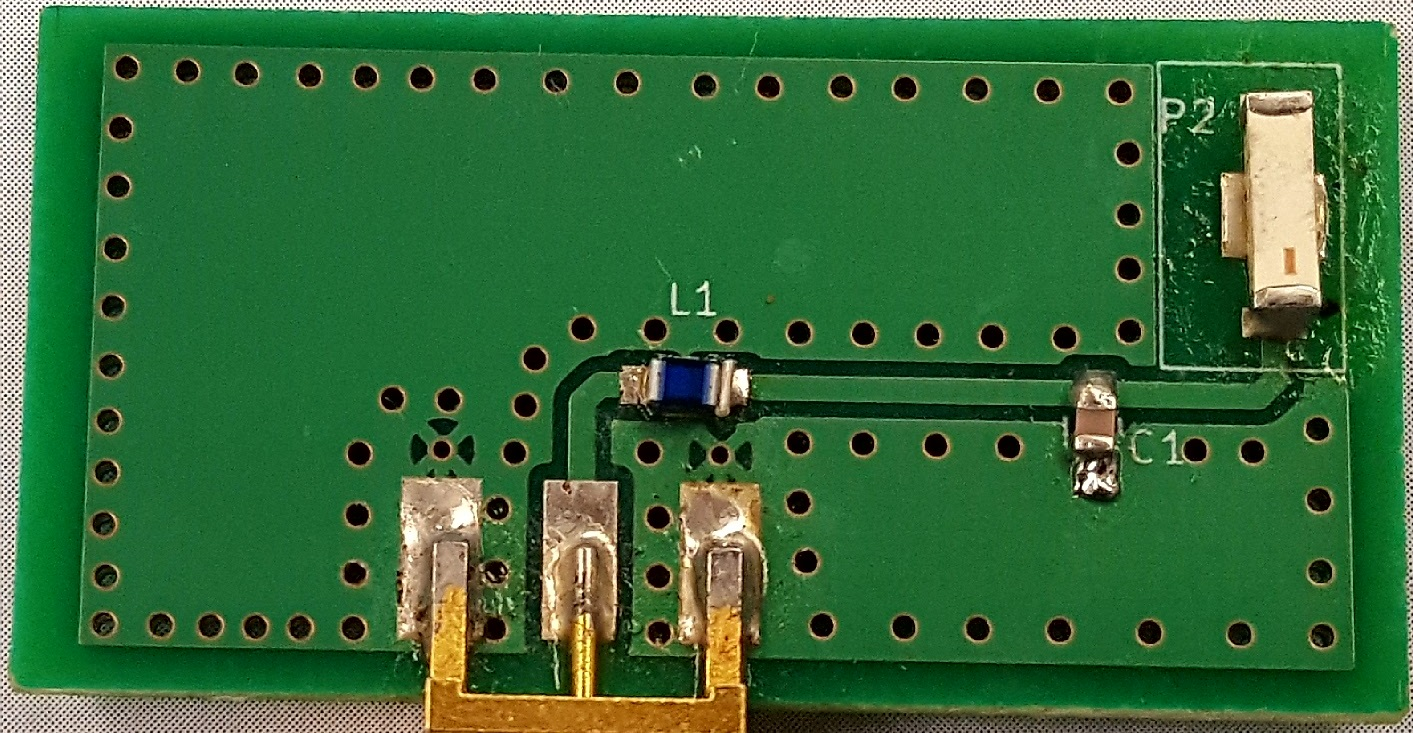
\includegraphics[width=0.4\textwidth]{2_4GHzChipAntenna.jpg}
\caption{Bluetooth 2.4 GHz Edge-Fed Chip Antenna}
\label{2.4 Chip}
\end{figure}


Each antenna needed to be tested in a variety of positions relative to the transmitted ground plane reference signal to determine the general directivity, polarization, and radiation pattern.  This means everything in the lab would ideally be in the same exact location for each iteration of testing.  The far-field lab testing measured the link loss of each antenna to determine which designs performed best relative to one another.   These antennas not only needed to transmit up to 50 feet but they needed to work properly in any position and behind obstacles.  The initial baseline testing used an RF link distance of 2 meters in direct line of sight with no direct obstacles, other than competing wireless signals and free space.  The ground plane reference antenna was positioned to direct its radiation in the general direction of the antenna under test (AUT) and all of the designs were thoroughly tested in reference of one another.  The same link loss gain test was conducted from across the lab with a RF distance of approximately 14 meters.  The results from both tests were excellent with a couple of the designs standing out above the rest.  All of the antennas were tunable except for one.

\begin{figure}[ht]	% There are several different modifiers that can be used in [].
\centering
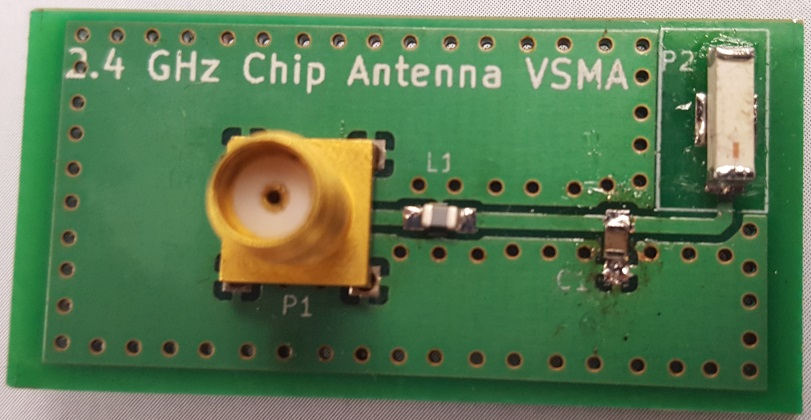
\includegraphics[width=0.4\textwidth]{2_4GHzVChipAntenna.jpg}
\caption{Bluetooth 2.4 GHz Chip Antenna}
\label{2.4 Chip}
\end{figure}

The next step was to test these antennas in the field at the De Anza Santa Cruz Senior Citizen Community.  With the reference ground plane antenna setup in a living room, all the antennas were tested and their performances measured in the actual home environment.  The first step was to establish the baseline parameters from across the living at an RF link distance of approximately 4 meters with no obstructions other than free space.  All the antenna designs were measured for link loss, polarization, and radiation pattern.  Next was to move slightly further way and down on the floor, behind a thick wooden table and chairs.  This simulated the position of the button had a person actually fallen in that position.  The results from both tests were quite good.  The next step of the process was to move the AUT across the length of the house into the bedroom.  This is where the performance of the antennas degraded.  With an RF link of approximately 16 meters, behind three metal walls, a television, and cabinets, the AUT’s could not receive a reasonable signal.  This is because the mobile homes at De Anza are metal, inside and out, so they act as Faraday cages, blocking our wireless signals.  When the AUT was moved to the open doorway, the signals were good.  However, when behind the obstruction of the walls, the signal was nearly buried in the noise floor.


Based on these results, it was determined that the small MIFA and chip corner-mount PCB designs performed best relative to the other designs.  They had better baseline impedances and less link loss.  These two antennas were then tuned with the appropriate impedance matching networks in the following revisions and additional testing was conducted from both inside and outside the lab.  These antennas had good performances up to 60 feet and easily reached our minimum specifications.  In the end, the antenna chosen for the button was the small MIFA since it performed approximately as well as the chip antenna and it is smaller, which makes it a better fit for use in the button device.

\begin{figure}[ht]	% There are several different modifiers that can be used in [].
\centering
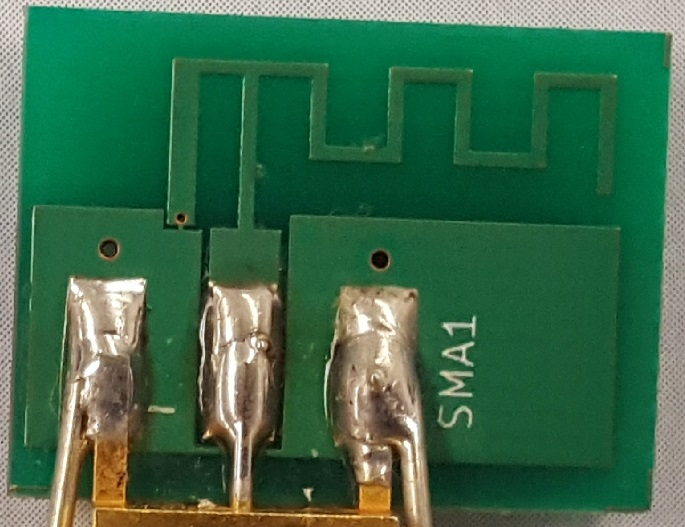
\includegraphics[width=0.4\textwidth]{2_4GHzSMIFAAntenna.jpg}
\caption{Bluetooth 2.4 GHz MIFA Antenna}
\label{2.4 Small MIFA}
\end{figure}


\begin{table*}[t]
  \centering
  \begin{tabular}{>{\bfseries}l|l l l l}
  \hline
    Topology & \multicolumn{1}{|c|}{2.39 GHz} & \multicolumn{1}{|c|}{2.43 GHz} & \multicolumn{1}{|c|}{2.46 GHz} & \multicolumn{1}{|c|}{2.50 GHz} \\
    \hline
    MIFA (Small, Slanted Feed) & \multicolumn{1}{|r|}{42.92 - j4.2, 16.7 pF} & \multicolumn{1}{|r|}{34.1 - j13.8, 5.1 pF} & \multicolumn{1}{|r|}{27.6 - j15.1, 4.4 pF} & \multicolumn{1}{|r|}{22.5 - j16.4, 3.8 pF} \\
    MIFA (Small) & \multicolumn{1}{|r|}{44.2 + j26.9, 1.8 pF} & \multicolumn{1}{|r|}{67.3 + j29.8, 1.9 pF} & \multicolumn{1}{|r|}{88.6 + j11.9, 745 pH} & \multicolumn{1}{|r|}{89.4 - j9.6, 7.7 pF} \\
    MIFA (Large, Slanted Feed) & \multicolumn{1}{|r|}{39.1 + j8.5, 555 pH} & \multicolumn{1}{|r|}{30.0 + j13.1, 857 pH} & \multicolumn{1}{|r|}{27.5 + j13.7, 896 pH} & \multicolumn{1}{|r|}{22.4 + j13.9, 880 pH} \\
    MIFA & \multicolumn{1}{|r|}{27.9 + j6.1, 411 pH} & \multicolumn{1}{|r|}{20.6 + j8.2, 532 pH} & \multicolumn{1}{|r|}{18.0 + j8.8, 567 pH} & \multicolumn{1}{|r|}{10.5 + j11.1, 692 pH} \\
    IFA (Left Arm) & \multicolumn{1}{|r|}{17.7 - j36.0, 1.84 pF} & \multicolumn{1}{|r|}{18.1 - j36.0, 1.81 pF} & \multicolumn{1}{|r|}{18.2 - j36.2, 1.78 pF} & \multicolumn{1}{|r|}{18.6 - j36.7, 1.73 pF} \\
    IFA (Right Arm) & \multicolumn{1}{|r|}{33.9 + j27.9, 1.86 pH} & \multicolumn{1}{|r|}{32.8 + j37.5, 2.46 pH} & \multicolumn{1}{|r|}{43.5 + j49.3, 3.19 pH} & \multicolumn{1}{|r|}{83.2 + j47.9, 3.01 pH} \\
    Patch & \multicolumn{1}{|r|}{157 + j540, 36.7 nH} & \multicolumn{1}{|r|}{723 + j463, 29.2 nH} & \multicolumn{1}{|r|}{716 - j37.0, 2.1 pF} & \multicolumn{1}{|r|}{420 - j196, 332 fF} \\
    RUFA & \multicolumn{1}{|r|}{107.1 - j46.8, 1.2 pF} & \multicolumn{1}{|r|}{76.1 - j60.8, 1.07 pF} & \multicolumn{1}{|r|}{58.4 - j58.6, 1.1 pF} & \multicolumn{1}{|r|}{44.6 - j53.1, 1.2 pF} \\
    Chip (Surface-Mount) & \multicolumn{1}{|r|}{32.6 - j43.2, 1.53 pF} & \multicolumn{1}{|r|}{31.2 - j39.6, 1.65 pF} & \multicolumn{1}{|r|}{30.2 - j37.2, 1.73 pF} & \multicolumn{1}{|r|}{28.6 - j34.7, 1.83 pF} \\ \hline
  \end{tabular} \newline
  \caption{Baseline Bluetooth 2.4 GHz Antenna Impedance Results}
\end{table*}

\begin{table*}[t]
  \centering
  \begin{tabular}{>{\bfseries}l|l l l l}
  \hline
    Topology & \multicolumn{1}{|c|}{902 MHz} & \multicolumn{1}{|c|}{910 MHz} & \multicolumn{1}{|c|}{915 MHz} & \multicolumn{1}{|c|}{2.50 MHz} \\
    \hline
    Planar IFA & \multicolumn{1}{|r|}{41.78 - j5.6, 6.1 pH} & \multicolumn{1}{|r|}{43.62 - j5.1, 6.3 pH} & \multicolumn{1}{|r|}{44.54 - j3.4, 6.4 pH} & \multicolumn{1}{|r|}{44.78 - j4.7, 5.9 pH} \\
    MIFA (Orthogonal) & \multicolumn{1}{|r|}{24.6 - j16.3, 1.13 pF} & \multicolumn{1}{|r|}{23.8 - j16.9, 2.01 pF} & \multicolumn{1}{|r|}{23.1 - j18.4, 2.24 pF} & \multicolumn{1}{|r|}{21.4 - j18.8, 2.31 pF} \\
    Chip (Surface-Mount) & \multicolumn{1}{|r|}{37.2 + j23.8, 1.48 pH} & \multicolumn{1}{|r|}{37.7 + j20.1, 1.44 pH} & \multicolumn{1}{|r|}{38.3 + j22.6, 1.41 pH} & \multicolumn{1}{|r|}{39.4 + j18.3, 1.55 pH} \\ \hline
  \end{tabular} \newline
  \caption{Baseline 915 MHz Antenna Impedance Results}
\end{table*}

\subsubsection{Base Station}

The antenna for the base station needed to operate in the chosen frequency band of 900 MHz frequency band to facilitate communication over a longer range of at least 300 feet, from one base station to another.  This lower frequency band is suitable for long distance RF links since the attenuation suffered by radio waves through free space decreases along with the operating frequency.  The base station antenna must also be capable of handling atmospheric loss due to gases and be able to navigate through outdoor environments, such as around trees and other obstructions.  One of the biggest advantages of this frequency band is that it’s “Near Line of Sight”, meaning better range can be achieved in this band than other ISM bands given the same obstructions.  Since there isn’t as much of a size constraint as with the button antenna, the base station antenna can be larger and external.  Several different PCB antenna layouts were designed with three standing out, plus a dual-band antenna operating at 915MHz-2.44GHz and a proven whip antenna as a 902-928 MHz reference

\begin{figure}[ht]	% There are several different modifiers that can be used in [].
\centering
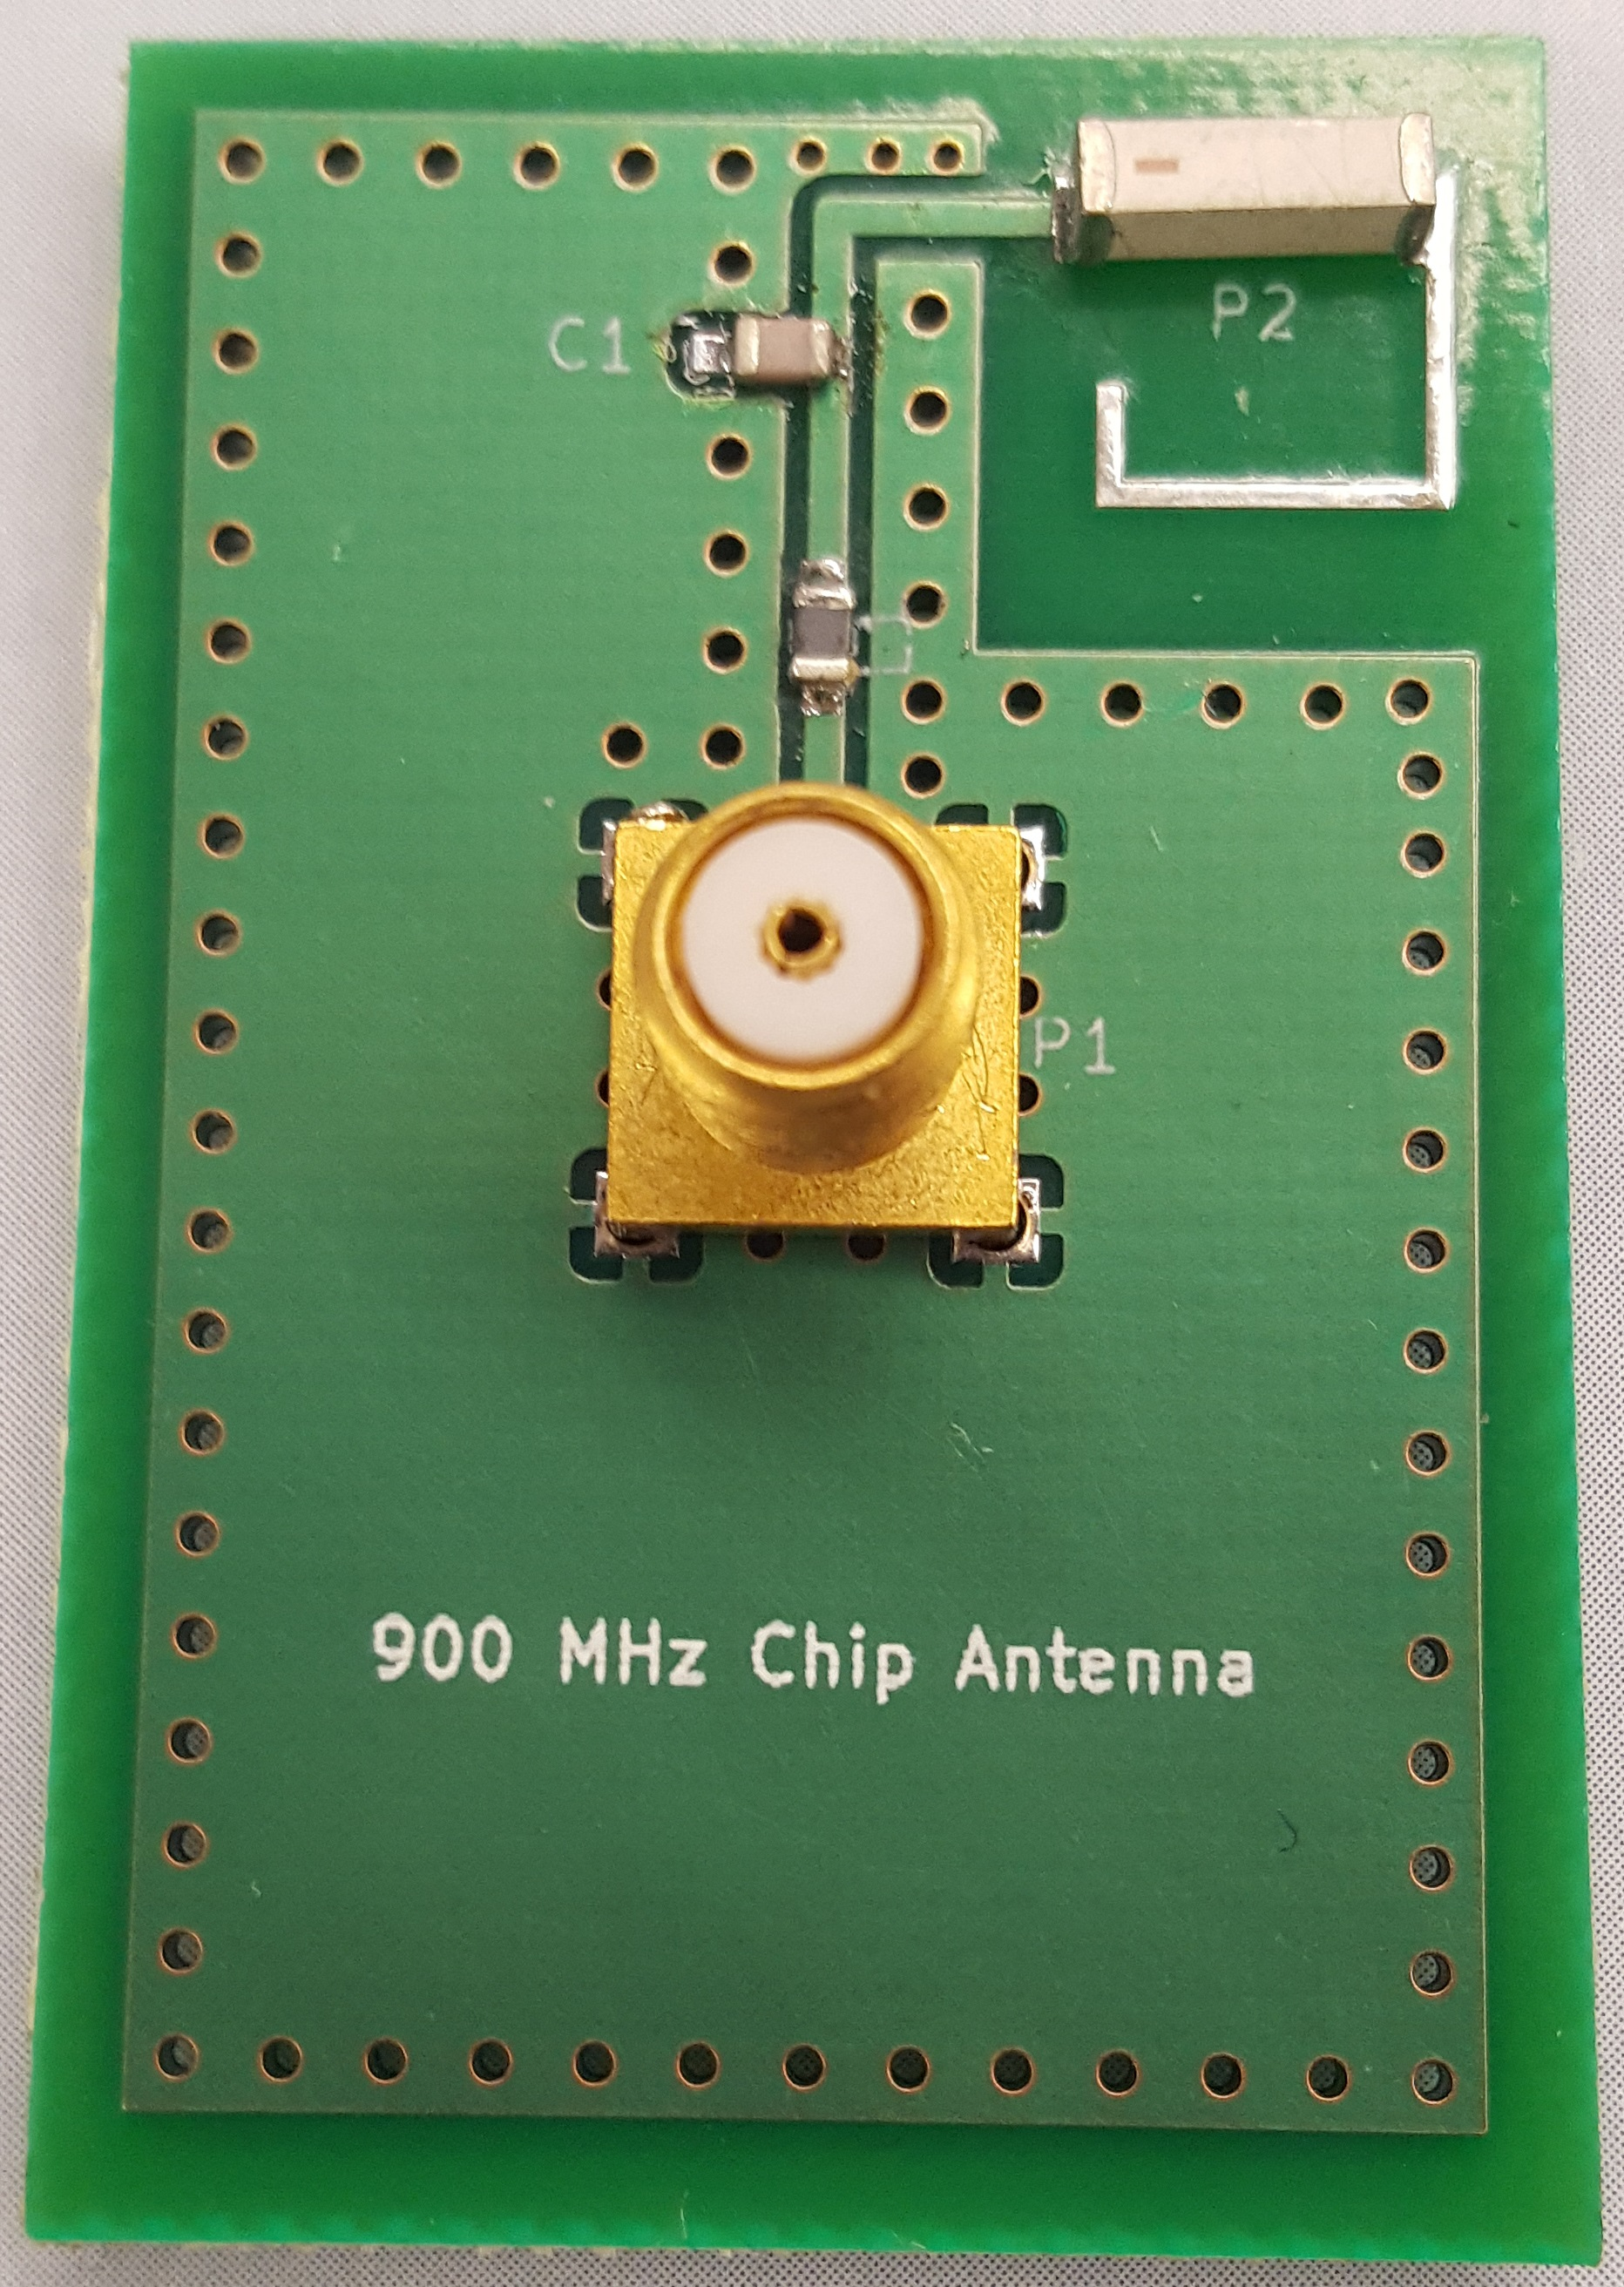
\includegraphics[width=0.4\textwidth]{900MHzChipAntenna.jpg}
\caption{Chip 915 MHz Antenna}
\label{915 MHz }
\end{figure}

The measuring and testing of the base station antennas was much the same as with the button 2.4 GHz antennas.  However, since these antennas are intended for longer transmission ranges from one house to another, field testing was conducted two separate times at the De Anza Santa Cruz Senior Citizens Community.  The first round of testing produced poor results because the antennas were only tested from within the houses.  For this initial test, the reference antenna was positioned near a bedroom window and the AUT was positioned from a far distance with an RF link distance over 500 feet and seven houses away.  This test produced zero results.  Next, the AUT was positioned from a closer RF link distance of approximately 300 feet and four houses away.  The reference antenna was then positioned in a bathroom with a much smaller window.  This produced poor results with the signal buried in the noise floor.

Further testing was then conducted in lab and this time with excellent results.  The reference antenna was positioned in the lab and directed towards the East.  The AUT’s were then taken outside to measure their performances, again using the Tektronix portable spectrum analyzer and laptop test bench.  This time the link loss for each design was minimal.  The antennas had excellent reception from over 300 feet, around corners to both the west and to the east, and down the hill to the north.  Only after moving far down the hill behind large redwood trees did the signal finally attenuate down to the noise floor, which was over the 300-foot minimum specification.  These also had excellent results reaching around the corner to the west, which in the opposite direction from the reference antenna radiation pattern.  This demonstrated the effectiveness of the designs and how the metal walls and mobile homes at De Anza truly do act as strong Faraday cages.

\begin{figure}[ht]
\centering
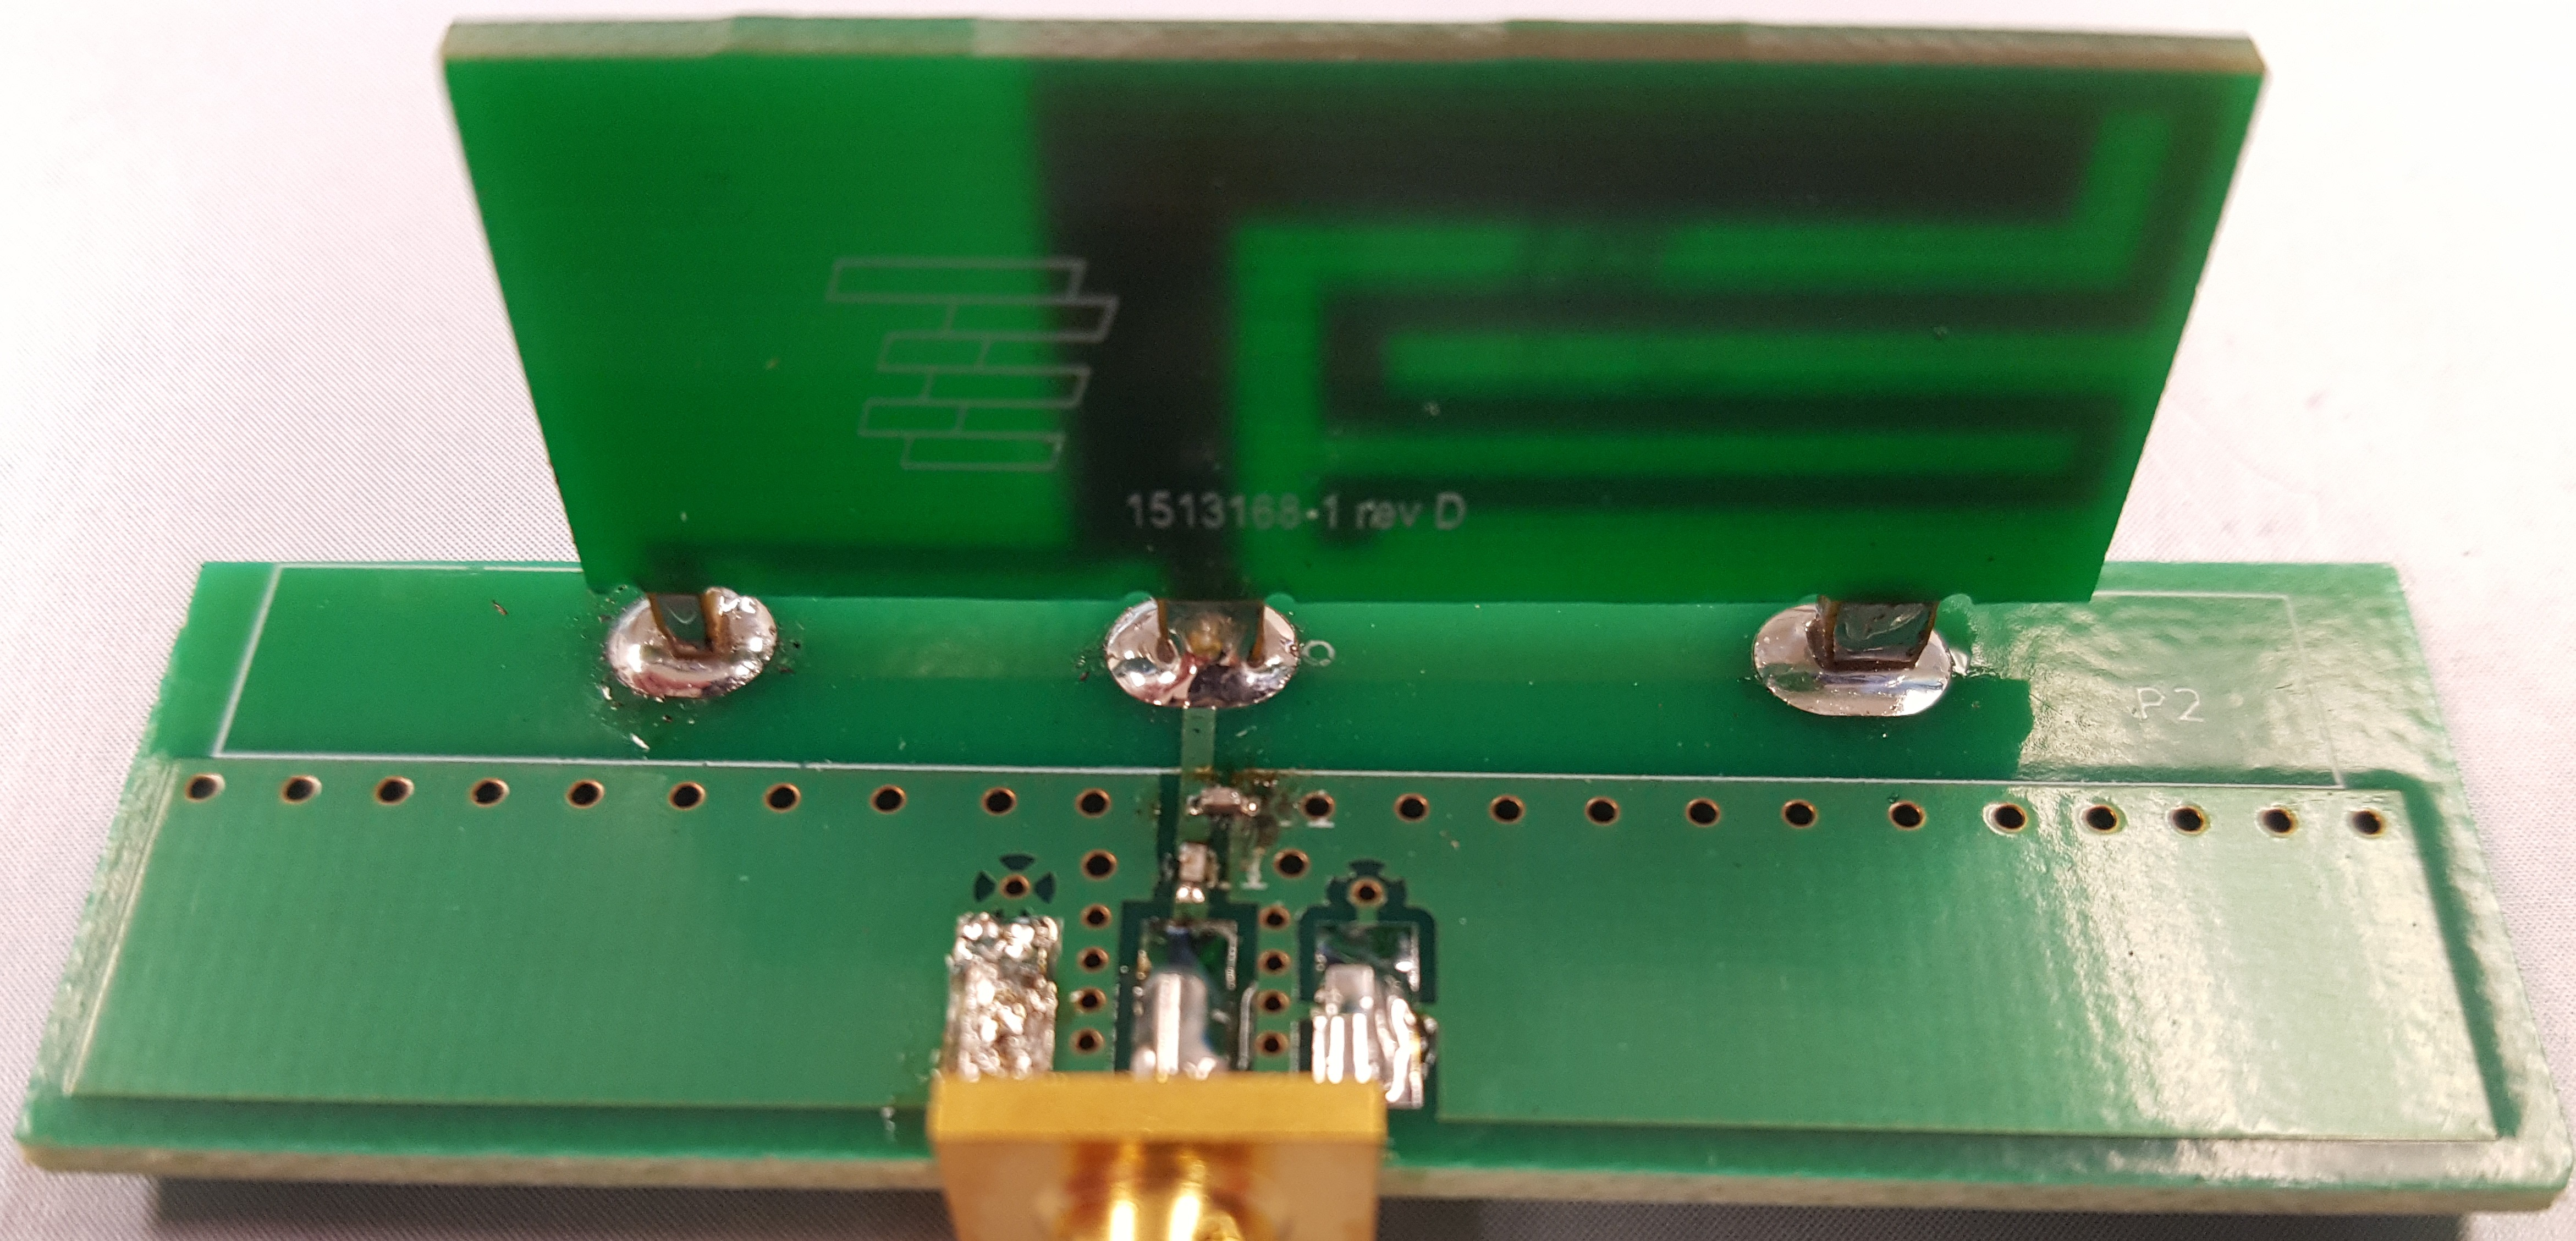
\includegraphics[width=0.4\textwidth]{900MHzMIFAAntenna.jpg}
\caption{MIFA 915 MHz Antenna}
\label{900 MHz MIFA}
\end{figure}

A second round of field testing was conducted at De Anza and this time the reference antenna was positioned in the living room with its radiation pattern directed to the west through the living room window.  Using the same portable test equipment, the AUT’s were taken outside and their performances measured from all around the entire neighborhood.  The All three designs performed very well with transmitting ranges up to 200 feet, sweeping from side to side in the line of sight.  However, with the reference transmitting antenna inside the house, the transmission range of 300 feet could not be met and there were no stable communications from the front of the house to the east.

The reference transmitting antenna was then placed directly above its inside location outside on top of the roof.  With this configuration of the radio-frequency link, the antennas performed exceedingly well and met all minimum specifications, including transmission ranges of over 300 feet.  They also now performed better from side to side and directly out the front of the house to the east.  This would be the optimum setup for the base station antennas, using simple repeaters placed on the roofs of the homes for THE optimum performance of up to 300 feet in all directions.  The antennas were still ineffective when directly behind a second metal home from the side and directly behind the directivity of the transmitted reference signal, which would be resolved with the proper strategic placement of basic repeaters.

\begin{figure}[ht]
\centering
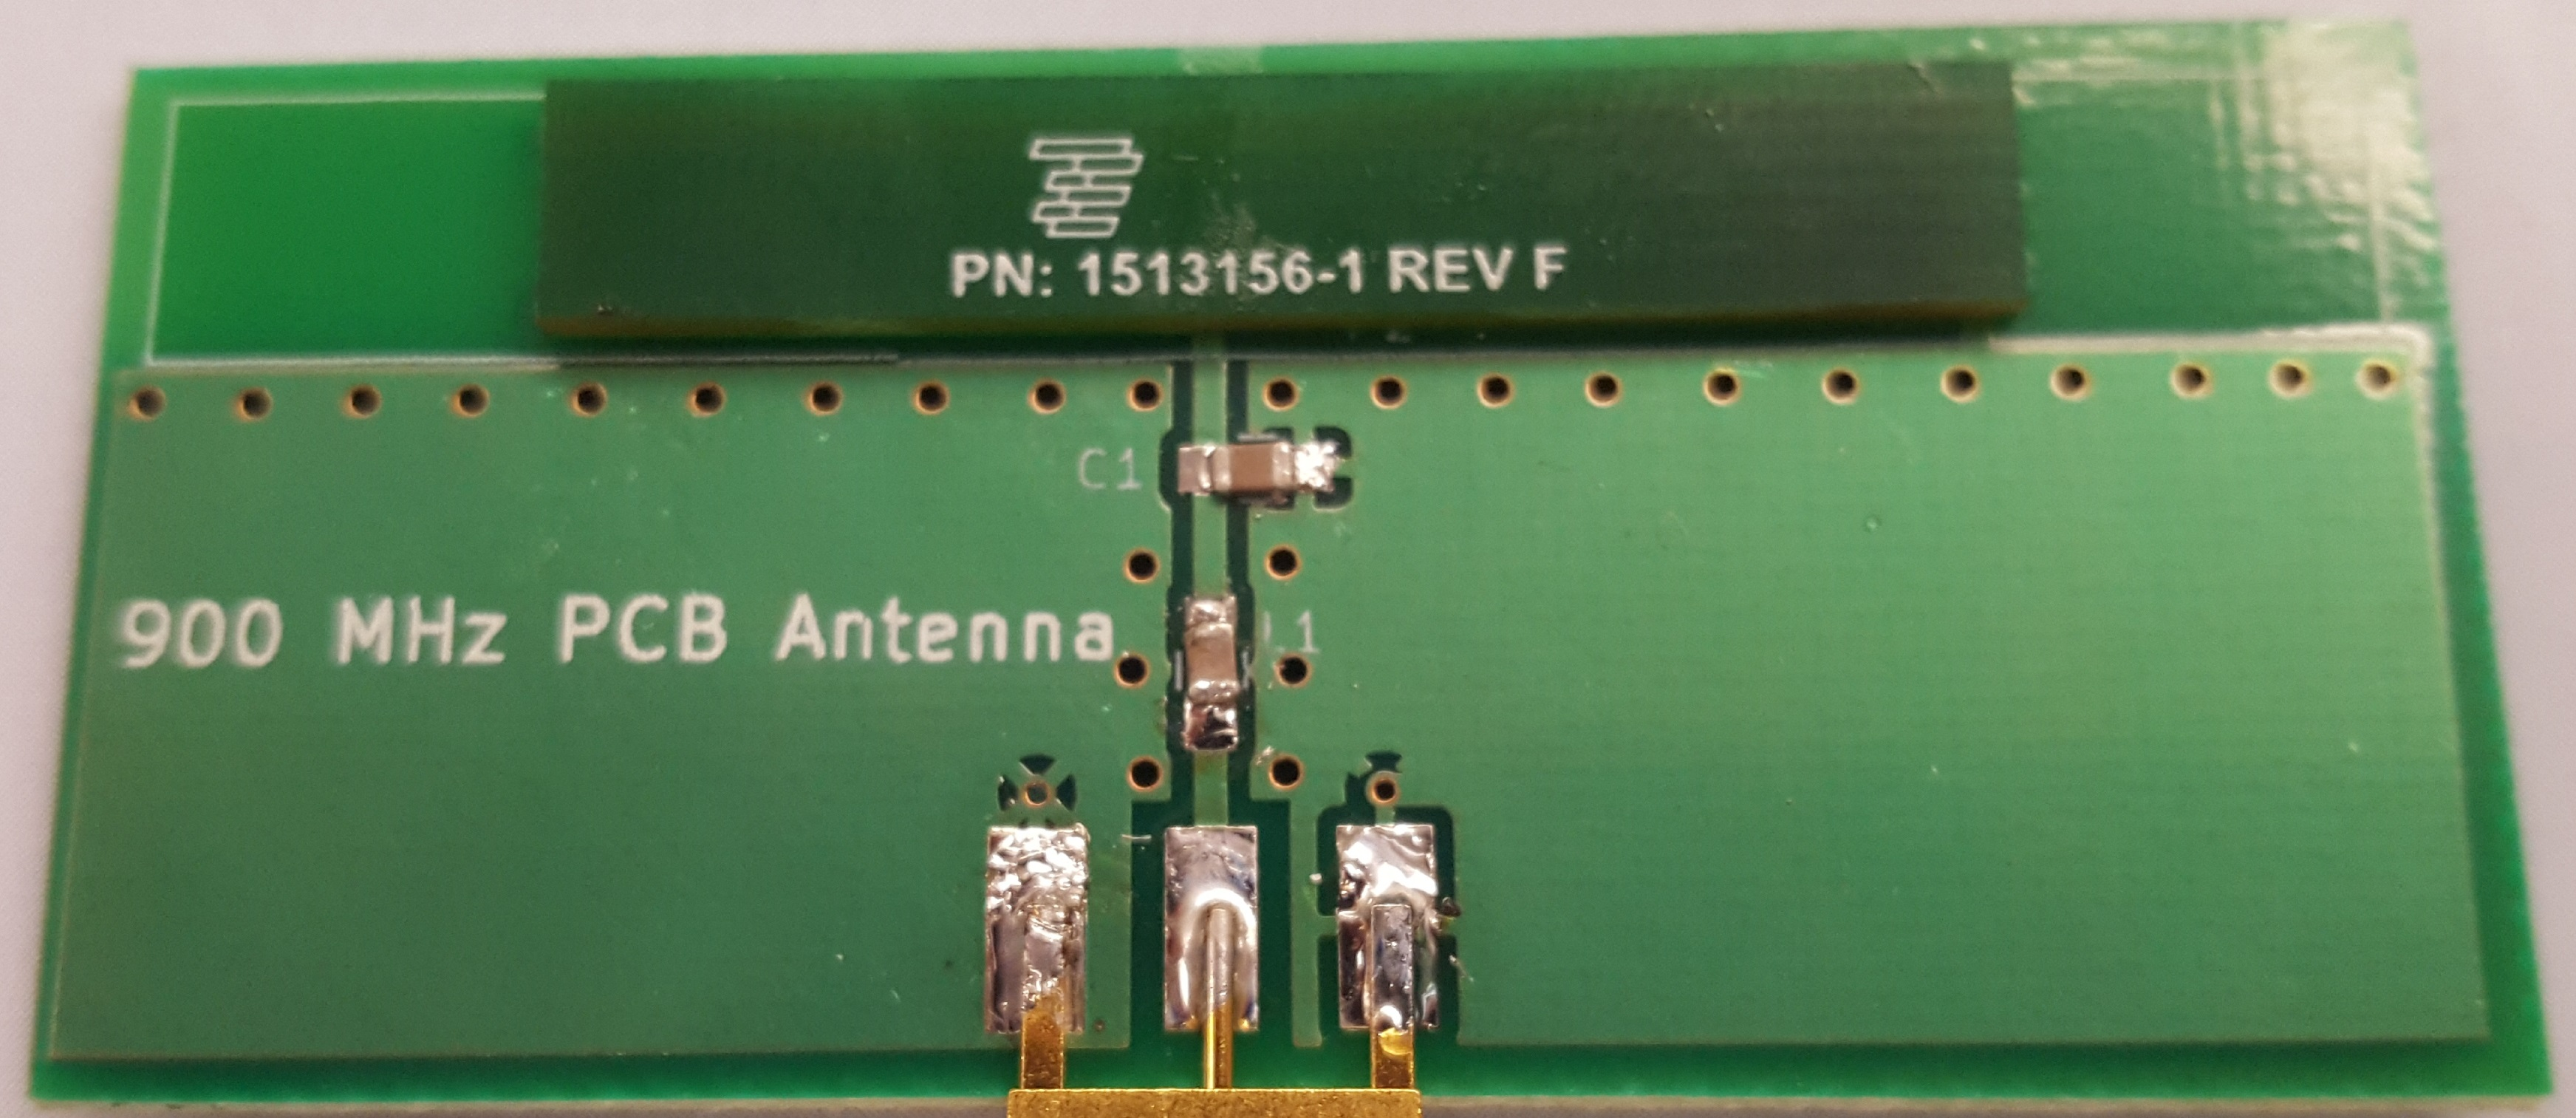
\includegraphics[width=0.4\textwidth]{900MHzRevFAntenna.jpg}
\caption{MIFA 915 MHz Antenna}
\label{900 MHz MIFA}
\end{figure}

All three tuned designs are compact, stable, sturdy, and easily integrated into the base station device, in any number of spatial configurations via the XBee SMA connection, depending on the XBee placement.  The smallest, least expensive, and most applicable of the designs is the surface mounted planar reversed inverted-f antenna.


\begin{table*}[t]
  \centering
  \begin{tabular}{>{\bfseries}l|l l l l}
  \hline
    Topology & \multicolumn{1}{|c|}{10 feet} & \multicolumn{1}{|c|}{25 feet} & \multicolumn{1}{|c|}{35 feet} & \multicolumn{1}{|c|}{50 feet} \\
    \hline
    MIFA (Small) & \multicolumn{1}{|r|}{-49 dBm} & \multicolumn{1}{|r|}{-56 dBm} & \multicolumn{1}{|r|}{-68 dBm} & \multicolumn{1}{|r|}{-77 dBm} \\
    Patch & \multicolumn{1}{|r|}{-54 dBm} & \multicolumn{1}{|r|}{-61 dBm} & \multicolumn{1}{|r|}{-72 dBm} & \multicolumn{1}{|r|}{-83 dBm} \\
    Chip (Surface-Mount) & \multicolumn{1}{|r|}{-47 dBm} & \multicolumn{1}{|r|}{-55 dBm} & \multicolumn{1}{|r|}{-65 dBm} & \multicolumn{1}{|r|}{-73 dBm} \\ \hline
  \end{tabular} \newline
  \caption{Tuned Bluetooth 2.4 GHz Antenna Link Loss Results}
\end{table*}

\begin{table*}[t]
  \centering
  \begin{tabular}{>{\bfseries}l|l l l l}
  \hline
    Topology & \multicolumn{1}{|c|}{75 feet} & \multicolumn{1}{|c|}{150 feet} & \multicolumn{1}{|c|}{225 feet} & \multicolumn{1}{|c|}{300 feet} \\
    \hline
    Planar IFA & \multicolumn{1}{|r|}{-74 dBm} & \multicolumn{1}{|r|}{-80 dBm} & \multicolumn{1}{|r|}{-94 dBm} & \multicolumn{1}{|r|}{-101 dBm} \\
    MIFA & \multicolumn{1}{|r|}{-73 dBm} & \multicolumn{1}{|r|}{-80 dBm} & \multicolumn{1}{|r|}{-91 dBm} & \multicolumn{1}{|r|}{-99 dBm} \\
    Chip (Surface-Mount) & \multicolumn{1}{|r|}{-76 dBm} & \multicolumn{1}{|r|}{-82 dBm} & \multicolumn{1}{|r|}{-94 dBm} & \multicolumn{1}{|r|}{-103 dBm} \\ \hline
  \end{tabular} \newline
  \caption{Tuned 915 MHz Antenna Link Loss Results}
\end{table*}

\subsection{Packaging}
Packaging was designed using a 3-dimensional modeling software. There were various pieces of software which could have been used, but there were trade-offs between the amount of time to learn one and have a finished packaged product in time. Various testing and research was conducted regarding which 3-D printing software to use and to name a few there was SolidWorks, FreeCAD, and Fusion 360. The most intuitive one to learn in a quick amount of time was Fusion 360 to design the encasements for the base station and the button device. 

Prior to receiving the software, rough sketches were made for the base station and button device. An important thing to remember was for the button device to be aesthetically appealing, compact, and jewelry-like. Collecting customer input narrowed down the button device to two designs in different colors for the customer to choose.  The designs for the base station had more freedom. Various versions were printed of both the base station and button device as it was difficult to perfect.

\begin{figure}[ht] 	% Several different modifiers can be used
\centering
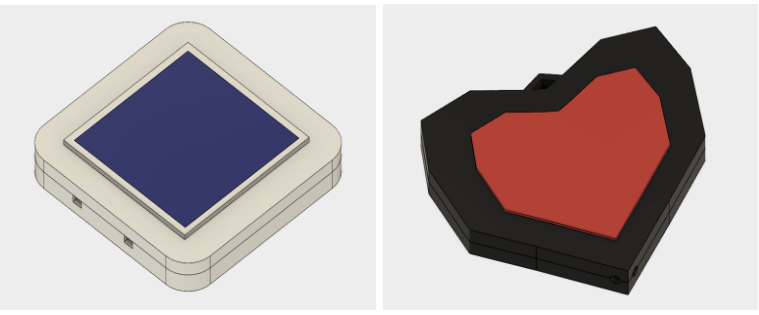
\includegraphics[width=0.4\textwidth]{Buttons.PNG}
\caption{Final designs for the button device}
\label{Ha-Ha Heart Buttons}
\end{figure}

\begin{figure}[ht] 	% Several different modifiers can be used
\centering
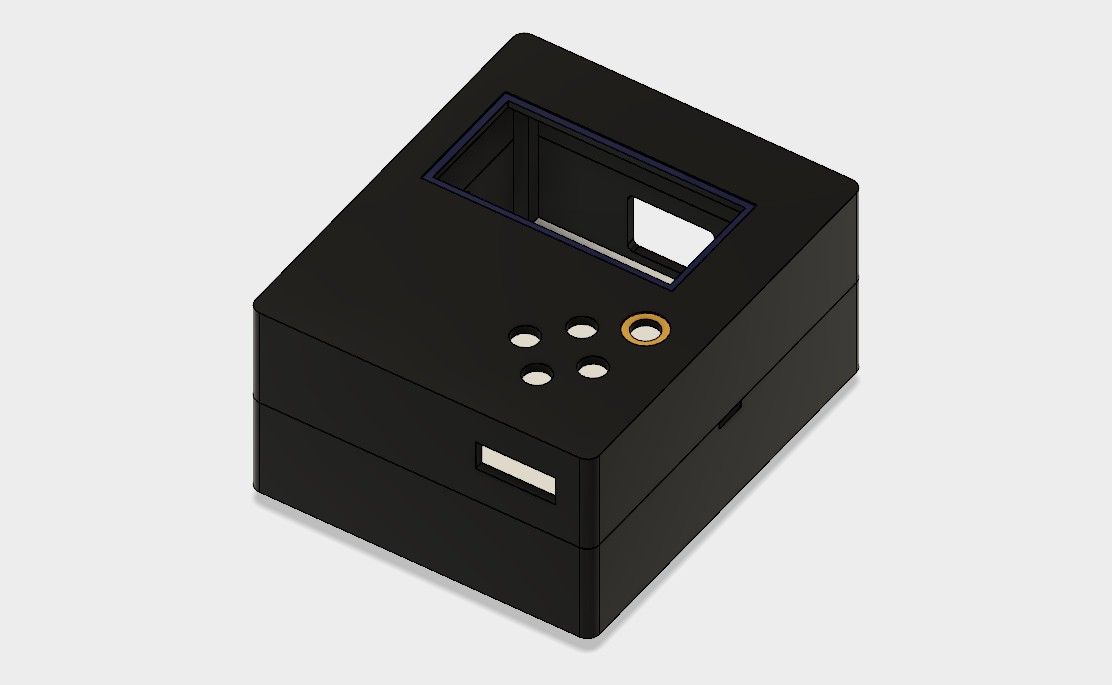
\includegraphics[width=0.4\textwidth]{Base.png}
\caption{Final design for base station}
\label{Ha-Ha Base Station}
\end{figure}

Cost\newline
The single cost of an entire prototype system brings the cost to about \$150. The cost of the system could decrease dramatically depending on the number of units produced, but with our small initial test community the cost is currently prohibitively high. To this end, we have identified a few parts that could be exchanged to bring down the cost significantly.
The main parts which could be replaced are the networking device  XBee-PRO, which costs around \$40, the NiMH 700mah rechargeable battery priced at \$13, and the LCD display with a value of \$10. The networking device is most likely to be replaced, as there are much less expensive alternatives, although at the cost of a high development time.

\section{Results}
The project has a fully integrated hardware prototype base station, and the base stations runs a working HA-HA application including the ability to send and interpret application messages. The functioning menu system interfaces with the application to set user preferences and initiate requests to other stations. The button is implemented on the development Blue-NRG1 board, as the final PCB design for it is incomplete. The power supply is in full working order, and it can support both the amplified audio alarm as well as triggering the external lighting system. The antenna designs have been evaluated and are ready to be used in the base station and the button. The button hardware is unfortunately incomplete and the cost of a single device is more than the goal of \$100 without mass production.

\section{Conclusion}

Although the design goal of no more than a \$100 was not met, substantial progress was achieved with a \$150 product cost.
After reviewing our options, it has been decided it would be beneficial to use an available off-the-shelf system on a chip (SoC) device, as they are mass produced and have many software libraries readily available which will reduce cost and development time. Another way to reduce cost would be to use an inexpensive networking device which can be attached to our current system, at the cost of a high development time.

After the design decisions regarding the new system are complete, a study will be conducted at the De Anza senior citizen community. This study will test the system and its design, particularly its aesthetic appeal, usability, and cost analysis to both the individual as well as the community, especially the savings resulting from a reduction in emergency services calls.

\appendices

\section{Bill of Materials}
%\newpage
\onecolumn
\begin{table}[]
  \centering
  %\caption{Bill of Materials}
    \begin{tabular}{|rrr|r|r|}
    \toprule
    \rowcolor[rgb]{ .663,  .816,  .557} \multicolumn{5}{|c|}{\textbf{Button}} \\
    \midrule
    \rowcolor[rgb]{ .608,  .761,  .902} \multicolumn{1}{|c|}{\textbf{Component}} & \multicolumn{1}{c|}{\textbf{Manufacturer}} & \multicolumn{1}{c|}{\textbf{Price/unit (US \$)}} & \multicolumn{1}{c|}{\textbf{Quantity}} & \multicolumn{1}{c|}{\textbf{Total for 1}} \\
    \midrule
    \multicolumn{1}{|l}{STMicroelectronics BlueNRG-132} & \multicolumn{1}{l}{STMicroelectronics} & \multicolumn{1}{r}{\$3.97 } & \multicolumn{1}{r}{1} & \$3.97 \\
    \multicolumn{1}{|l}{ST BlueNRG-1 Balun} & \multicolumn{1}{l}{STMicroelectronics} & \multicolumn{1}{r}{\$0.51 } & \multicolumn{1}{r}{1} & \$0.51 \\
    \multicolumn{1}{|l}{Battery (Energizer CR2032)} & \multicolumn{1}{l}{Energizer} & \multicolumn{1}{r}{\$0.34 } & \multicolumn{1}{r}{1} & \$0.34 \\
    \multicolumn{1}{|l}{Battery Holder} & \multicolumn{1}{l}{Keystone Electronics} & \multicolumn{1}{r}{\$0.31 } & \multicolumn{1}{r}{1} & \$0.31 \\
    \multicolumn{1}{|l}{Button/Tactile Switch} & \multicolumn{1}{l}{TE Connectivity} & \multicolumn{1}{r}{\$0.10 } & \multicolumn{1}{r}{1} & \$0.10 \\
    \multicolumn{1}{|l}{Schottky Diode (x2)} & \multicolumn{1}{l}{Comchip} & \multicolumn{1}{r}{\$0.46 } & \multicolumn{1}{r}{2} & \$0.92 \\
    \multicolumn{1}{|l}{Low-Power LEDs (x2)} & \multicolumn{1}{l}{Rohm} & \multicolumn{1}{r}{\$0.55 } & \multicolumn{1}{r}{2} & \$1.10 \\
    \multicolumn{1}{|l}{TI LDO Regulator} & \multicolumn{1}{l}{TI} & \multicolumn{1}{r}{\$0.64 } & \multicolumn{1}{r}{1} & \$0.64 \\
    \multicolumn{1}{|l}{Inductor, 10uH} & \multicolumn{1}{l}{Samsung} & \multicolumn{1}{r}{\$0.15 } & \multicolumn{1}{r}{1} & \$0.15 \\
    \multicolumn{1}{|l}{Abracon Crystal Oscillator, 32.768kHz (2-SMD)} & \multicolumn{1}{l}{Abracon} & \multicolumn{1}{r}{\$0.71 } & \multicolumn{1}{r}{1} & \$0.71 \\
    \multicolumn{1}{|l}{Kyocera Crystal Oscillator, 32MHz (4-SMD)} & \multicolumn{1}{l}{AVX/Kyocera} & \multicolumn{1}{r}{\$1.24 } & \multicolumn{1}{r}{1} & \$1.24 \\
    \multicolumn{1}{|l}{RF Matching Components (Pi-Network)} & \multicolumn{1}{l}{Assorted} & \multicolumn{1}{r}{\$0.10 } & \multicolumn{1}{r}{3} & \$0.30 \\
    \multicolumn{1}{|l}{Miscellaneous [C0G] Capacitors (x23)} & \multicolumn{1}{l}{Murata} & \multicolumn{1}{r}{\$0.10 } & \multicolumn{1}{r}{23} & \$2.30 \\
    \multicolumn{1}{|l}{Resistors (x9)} & \multicolumn{1}{l}{Yageo} & \multicolumn{1}{r}{\$0.10 } & \multicolumn{1}{r}{9} & \$0.90 \\
    \multicolumn{1}{|l}{PCB} & \multicolumn{1}{l}{Bay Area Circuits} & \multicolumn{1}{r}{} & \multicolumn{1}{r}{1} & \$0.00 \\
    \multicolumn{1}{|l}{Packaging} & \multicolumn{1}{l}{3D-Printed ABS (?)} & \multicolumn{1}{r}{} & \multicolumn{1}{r}{1} & \$0.00 \\
\cmidrule{4-5}          &       &       & \cellcolor[rgb]{ .608,  .761,  .902} \textbf{Subtotal} & \cellcolor[rgb]{ .608,  .761,  .902} \textbf{\$13.49} \\
    \midrule
          &       & \multicolumn{1}{r}{} & \multicolumn{1}{r}{} &  \\
    \midrule
    \end{tabular}%
  \label{tab:addlabel}%
\end{table}%
\begin{table}[]
  \centering
    \begin{tabular}{|rrr|r|r|}
    \rowcolor[rgb]{ .663,  .816,  .557} \multicolumn{5}{|c|}{\textbf{Base Station}} \\
    \midrule
    \rowcolor[rgb]{ .608,  .761,  .902} \multicolumn{1}{|c|}{\textbf{Part Name}} & \multicolumn{1}{c|}{\textbf{Manufacturer}} &       & \multicolumn{1}{c|}{\textbf{Quantity}} & \multicolumn{1}{c|}{\textbf{Total for 1}} \\
    \midrule
    \multicolumn{1}{|l}{KS-01Q-01} & \multicolumn{1}{l}{E-Switch} & \multicolumn{1}{r}{} & \multicolumn{1}{r}{1} & \$0.52  \\
    \multicolumn{1}{|l}{KS-01Q-01} & \multicolumn{1}{l}{E-Switch} & \multicolumn{1}{r}{} & \multicolumn{1}{r}{1} & \$0.52  \\
    \multicolumn{1}{|l}{KS-01Q-01} & \multicolumn{1}{l}{E-Switch} & \multicolumn{1}{r}{} & \multicolumn{1}{r}{1} & \$0.52  \\
    \multicolumn{1}{|l}{KS-01Q-01} & \multicolumn{1}{l}{E-Switch} & \multicolumn{1}{r}{} & \multicolumn{1}{r}{1} & \$0.52  \\
    \multicolumn{1}{|l}{KS-01Q-01} & \multicolumn{1}{l}{E-Switch} & \multicolumn{1}{r}{} & \multicolumn{1}{r}{1} & \$0.52  \\
    \multicolumn{1}{|l}{GRM1555C1H100FA01D} & \multicolumn{1}{l}{Murata} & \multicolumn{1}{r}{} & \multicolumn{1}{r}{1} & \$0.10  \\
    \multicolumn{1}{|l}{GRM1555C1H100FA01D} & \multicolumn{1}{l}{Murata} & \multicolumn{1}{r}{} & \multicolumn{1}{r}{1} & \$0.10  \\
    \multicolumn{1}{|l}{GRM155R61A105KE01D} & \multicolumn{1}{l}{Murata} & \multicolumn{1}{r}{} & \multicolumn{1}{r}{1} & \$0.10  \\
    \multicolumn{1}{|l}{GRM155R61H104JE14D} & \multicolumn{1}{l}{Murata} & \multicolumn{1}{r}{} & \multicolumn{1}{r}{1} & \$0.10  \\
    \multicolumn{1}{|l}{GRM155R61H104JE14D} & \multicolumn{1}{l}{Murata} & \multicolumn{1}{r}{} & \multicolumn{1}{r}{1} & \$0.10  \\
    \multicolumn{1}{|l}{GRM155R61H104JE14D} & \multicolumn{1}{l}{Murata} & \multicolumn{1}{r}{} & \multicolumn{1}{r}{1} & \$0.10  \\
    \multicolumn{1}{|l}{04026D475KAT2A} & \multicolumn{1}{l}{AVX} & \multicolumn{1}{r}{} & \multicolumn{1}{r}{1} & \$0.13  \\
    \multicolumn{1}{|l}{GRM155R61H104JE14D} & \multicolumn{1}{l}{Murata} & \multicolumn{1}{r}{} & \multicolumn{1}{r}{1} & \$0.10  \\
    \multicolumn{1}{|l}{GRM155R61A225KE95D} & \multicolumn{1}{l}{Murata} & \multicolumn{1}{r}{} & \multicolumn{1}{r}{1} & \$0.10  \\
    \multicolumn{1}{|l}{GRM155R71H103JA88D} & \multicolumn{1}{l}{Murata} & \multicolumn{1}{r}{} & \multicolumn{1}{r}{1} & \$0.10  \\
    \multicolumn{1}{|l}{GRM155R61A105KE01D} & \multicolumn{1}{l}{Murata} & \multicolumn{1}{r}{} & \multicolumn{1}{r}{1} & \$0.10  \\
    \multicolumn{1}{|l}{GRM155R61A105KE01D} & \multicolumn{1}{l}{Murata} & \multicolumn{1}{r}{} & \multicolumn{1}{r}{1} & \$0.10  \\
    \multicolumn{1}{|l}{GRM155R61A105KE01D} & \multicolumn{1}{l}{Murata} & \multicolumn{1}{r}{} & \multicolumn{1}{r}{1} & \$0.10  \\
    \multicolumn{1}{|l}{GRM1555C1H470FA01D} & \multicolumn{1}{l}{Murata} & \multicolumn{1}{r}{} & \multicolumn{1}{r}{1} & \$0.10  \\
    \multicolumn{1}{|l}{GRM155R61A105KE01D} & \multicolumn{1}{l}{Murata} & \multicolumn{1}{r}{} & \multicolumn{1}{r}{1} & \$0.10  \\
    \multicolumn{1}{|l}{GRM155C80J106ME11D} & \multicolumn{1}{l}{Murata} & \multicolumn{1}{r}{} & \multicolumn{1}{r}{1} & \$0.16  \\
    \multicolumn{1}{|l}{CFAH1604A-TMI-JT} & \multicolumn{1}{l}{Crystalfontz} & \multicolumn{1}{r}{} & \multicolumn{1}{r}{1} & \$9.48  \\
    \multicolumn{1}{|l}{PREC016SAAN-RC} & \multicolumn{1}{l}{Sullins} & \multicolumn{1}{r}{} & \multicolumn{1}{r}{1} & \$0.30  \\
    \multicolumn{1}{|l}{310-87-116-41-001101} & \multicolumn{1}{l}{Preci-Dip} & \multicolumn{1}{r}{} & \multicolumn{1}{r}{1} & \$0.91  \\
    \multicolumn{1}{|l}{BLM18PG181SN1D} & \multicolumn{1}{l}{Murata} & \multicolumn{1}{r}{} & \multicolumn{1}{r}{1} & \$0.10  \\
    \multicolumn{1}{|l}{302-R201} & \multicolumn{1}{l}{On Shore} & \multicolumn{1}{r}{} & \multicolumn{1}{r}{1} & \$0.62  \\
    \multicolumn{1}{|l}{10118194-0001LF} & \multicolumn{1}{l}{Amphenol} & \multicolumn{1}{r}{} & \multicolumn{1}{r}{1} & \$0.46  \\
    \multicolumn{1}{|l}{36401E9N1ATDF} & \multicolumn{1}{l}{TE Connectivity} & \multicolumn{1}{r}{} & \multicolumn{1}{r}{1} & \$0.10  \\
    \multicolumn{1}{|l}{CV201210-4R7K} & \multicolumn{1}{l}{Bourns} & \multicolumn{1}{r}{} & \multicolumn{1}{r}{1} & \$0.10  \\
    \multicolumn{1}{|l}{OSTTE020104} & \multicolumn{1}{l}{On Shore} & \multicolumn{1}{r}{} & \multicolumn{1}{r}{1} & \$0.35  \\
    \multicolumn{1}{|l}{OSTTE020105} & \multicolumn{1}{l}{On Shore} & \multicolumn{1}{r}{} & \multicolumn{1}{r}{1} & \$0.35  \\
    \multicolumn{1}{|l}{OSTTE020106} & \multicolumn{1}{l}{On Shore} & \multicolumn{1}{r}{} & \multicolumn{1}{r}{1} & \$0.35  \\
    \multicolumn{1}{|l}{OSTTE020106} & \multicolumn{1}{l}{On Shore} & \multicolumn{1}{r}{} & \multicolumn{1}{r}{1} & \$0.35  \\
    \multicolumn{1}{|l}{IRLML2502TRPBF} & \multicolumn{1}{l}{Infineon} & \multicolumn{1}{r}{} & \multicolumn{1}{r}{1} & \$0.46  \\
    \multicolumn{1}{|l}{RCS04021K00FKED} & \multicolumn{1}{l}{Vishay} & \multicolumn{1}{r}{} & \multicolumn{1}{r}{1} & \$0.11  \\
    \multicolumn{1}{|l}{RCS0402100KFKED} & \multicolumn{1}{l}{Vishay} & \multicolumn{1}{r}{} & \multicolumn{1}{r}{1} & \$0.11  \\
    \multicolumn{1}{|l}{RCS0402100RFKED} & \multicolumn{1}{l}{Vishay} & \multicolumn{1}{r}{} & \multicolumn{1}{r}{1} & \$0.11  \\
    \multicolumn{1}{|l}{RCS04021K00FKED} & \multicolumn{1}{l}{Vishay} & \multicolumn{1}{r}{} & \multicolumn{1}{r}{1} & \$0.11  \\
    \multicolumn{1}{|l}{3309W-1-103} & \multicolumn{1}{l}{Bourns} & \multicolumn{1}{r}{} & \multicolumn{1}{r}{1} & \$0.56  \\
    \multicolumn{1}{|l}{ATSAMB11G18A-MU-T} & \multicolumn{1}{l}{Microchip (Atmel)} & \multicolumn{1}{r}{} & \multicolumn{1}{r}{1} & \$3.51  \\
    \multicolumn{1}{|l}{XBP9B-DMST-002} & \multicolumn{1}{l}{Digi} & \multicolumn{1}{r}{} & \multicolumn{1}{r}{1} & \$39.00  \\
    \multicolumn{1}{|l}{ABS07AIG-32.768KHZ-6-T} & \multicolumn{1}{l}{Abracon} & \multicolumn{1}{r}{} & \multicolumn{1}{r}{1} & \$0.71  \\
    \multicolumn{1}{|l}{CX3225SB26000D0FFFCC} & \multicolumn{1}{l}{Kyocera (AVX)} & \multicolumn{1}{r}{} & \multicolumn{1}{r}{1} & \$0.76  \\
    \multicolumn{1}{|l}{ANT-916-PML} & \multicolumn{1}{l}{Linx} & \multicolumn{1}{r}{} & \multicolumn{1}{r}{1} & \$8.12  \\
    \multicolumn{1}{|l}{132193} & \multicolumn{1}{l}{Amphenol} & \multicolumn{1}{r}{} & \multicolumn{1}{r}{1} & \$6.12  \\
          &       & \multicolumn{1}{r}{} & \multicolumn{1}{r}{} &  \\
\cmidrule{4-5}          &       &       & \cellcolor[rgb]{ .608,  .761,  .902} \textbf{Subtotal} & \cellcolor[rgb]{ .608,  .761,  .902} \textbf{\$77.43 } \\
    \midrule
          &       & \multicolumn{1}{r}{} & \multicolumn{1}{r}{} &  \\
    \midrule
    \end{tabular}%
  \label{tab:addlabel}%
\end{table}%
\begin{table}[]
  \centering
   \begin{tabular}{|rrr|r|r|}
    \rowcolor[rgb]{ .663,  .816,  .557} \multicolumn{5}{|c|}{\textbf{Power Supply}} \\
    \midrule
    \rowcolor[rgb]{ .608,  .761,  .902} \multicolumn{1}{|l}{\textbf{Description}} & \multicolumn{1}{l}{\textbf{Manufacturer }} & \multicolumn{1}{l}{\textbf{Manufacturer ID}} & \multicolumn{1}{l}{\textbf{\# of units}} & \multicolumn{1}{l|}{\textbf{Price }} \\
    \multicolumn{1}{|l}{AC/DC WALL MOUNT ADAPTER 12V 10W} & \multicolumn{1}{l}{Qualtek} & \multicolumn{1}{l}{QFWB-10-12-US01} & \multicolumn{1}{r}{1} & 7.96 \\
    \multicolumn{1}{|l}{BATTERY PACK NIMH 4.8V 700MAH} & \multicolumn{1}{l}{Panasonic - BSG} & \multicolumn{1}{l}{HHR70AAAB8F2X2} & \multicolumn{1}{r}{1} & 12.84 \\
    \multicolumn{1}{|l}{PWR ENT RCPT IEC320-C14 PNL SLDR} & \multicolumn{1}{l}{Qualtek} & \multicolumn{1}{l}{703W-00/53} & \multicolumn{1}{r}{1} & 0.99 \\
    \multicolumn{1}{|l}{PWR ENT RCPT NEMA5-15 PANEL IDC} & \multicolumn{1}{l}{Qualtek} & \multicolumn{1}{l}{739W-X2/03} & \multicolumn{1}{r}{1} & 1.01 \\
    \multicolumn{1}{|l}{CONN PWR JACK 2.1X5.5MM SOLDER} & \multicolumn{1}{l}{MPD (Memory Protection Devices)} & \multicolumn{1}{l}{EJ508A} & \multicolumn{1}{r}{1} & 0.82 \\
    \multicolumn{1}{|l}{DIODE SCHOTTKY 30V 1A DO41} & \multicolumn{1}{l}{Diodes Incorporated} & \multicolumn{1}{l}{1N5818-T} & \multicolumn{1}{r}{7} & 2.59 \\
    \multicolumn{1}{|l}{CAP CER 0.1UF 50V X7R RADIAL} & \multicolumn{1}{l}{Vishay BC Components} & \multicolumn{1}{l}{K104K15X7RF5TL2} & \multicolumn{1}{r}{5} & 1.15 \\
    \multicolumn{1}{|l}{CAP CER 1UF 50V Y5V RADIAL} & \multicolumn{1}{l}{Vishay BC Components} & \multicolumn{1}{l}{K105Z20Y5VF5TH5} & \multicolumn{1}{r}{3} & 0.99 \\
    \multicolumn{1}{|l}{SWITCH ROCKER SPST 15A 125V} & \multicolumn{1}{l}{E-Switch} & \multicolumn{1}{l}{R1966ABLKBLKFR} & \multicolumn{1}{r}{1} & 1.37 \\
    \multicolumn{1}{|l}{IC REG LINEAR ADJ 1.5A TO220AB} & \multicolumn{1}{l}{STMicroelectronics} & \multicolumn{1}{l}{LM317T} & \multicolumn{1}{r}{1} & 0.53 \\
    \multicolumn{1}{|l}{IC REG BCK BST INV ADJ 1.5A 8DIP} & \multicolumn{1}{l}{Texas Instruments} & \multicolumn{1}{l}{MC34063AP} & \multicolumn{1}{r}{1} & 0.58 \\
    \multicolumn{1}{|l}{IC REG BUCK 3.3V 0.5A 8DIP} & \multicolumn{1}{l}{Microchip Technolog} & \multicolumn{1}{l}{LM2672N-3.3/NOPB} & \multicolumn{1}{r}{1} & 1.49 \\
    \multicolumn{1}{|l}{IC AMP AUDIO PWR 1W MONO AB 8DIP} & \multicolumn{1}{l}{Texas Instruments} & \multicolumn{1}{l}{LM386N-4/NOPB} & \multicolumn{1}{r}{1} & 0.98 \\
    \multicolumn{1}{|l}{TRIAC SENS GATE 200V 4A TO225AA} & \multicolumn{1}{l}{Littelfuse Inc.} & \multicolumn{1}{l}{2N6071BG} & \multicolumn{1}{r}{1} & 0.69 \\
    \multicolumn{1}{|l}{OPTOISOLATOR 4.17KV TRIAC 6DIP} & \multicolumn{1}{l}{Fairchild/ON Semiconductor} & \multicolumn{1}{l}{MOC3043M} & \multicolumn{1}{r}{1} & 1.09 \\
    \multicolumn{1}{|l}{RES 1K OHM 1/4W 5\% AXIAL} & \multicolumn{1}{l}{Stackpole Electronics Inc.} & \multicolumn{1}{l}{CF14JT1K00} & \multicolumn{1}{r}{4} & 0.4 \\
    \multicolumn{1}{|l}{RES 180 OHM 1/4W 5\% AXIAL} & \multicolumn{1}{l}{Stackpole Electronics Inc.} & \multicolumn{1}{l}{CF14JT180R} & \multicolumn{1}{r}{2} & 0.2 \\
    \multicolumn{1}{|l}{RES 0.22 OHM 1W 5\% AXIAL} & \multicolumn{1}{l}{Yageo} & \multicolumn{1}{l}{KNP100JR-73-0R22} & \multicolumn{1}{r}{1} & 0.33 \\
    \multicolumn{1}{|l}{RES 10K OHM 1/4W 5\% AXIAL} & \multicolumn{1}{l}{Stackpole Electronics Inc.} & \multicolumn{1}{l}{CF14JT10K0} & \multicolumn{1}{r}{1} & 0.1 \\
    \multicolumn{1}{|l}{RES 620 OHM 1/4W 5\% AXIAL} & \multicolumn{1}{l}{Stackpole Electronics Inc.} & \multicolumn{1}{l}{CF14JT620} & \multicolumn{1}{r}{1} & 0.1 \\
    \multicolumn{1}{|l}{FUSE BRD MNT 500MA 350VAC 100VD
} & \multicolumn{1}{l}{Bel Fuse Inc.} & \multicolumn{1}{l}{0697H0500-01} & \multicolumn{1}{r}{2} & 0.62 \\
    \multicolumn{1}{|l}{DIODE ZENER 3.3V 300MW SOD323} & \multicolumn{1}{l}{ON Semiconductor} & \multicolumn{1}{l}{MM3Z3V3T1G} & \multicolumn{1}{r}{1} & 0.14 \\
    \multicolumn{1}{|l}{DIODE ZENER 5V 250MW SOT23} & \multicolumn{1}{l}{Nexperia USA Inc.} & \multicolumn{1}{l}{PLVA650A,215} & \multicolumn{1}{r}{1} & 0.38 \\
    \multicolumn{1}{|l}{DIODE ZENER 12V 200MW SOD323} & \multicolumn{1}{l}{ON Semiconductor} & \multicolumn{1}{l}{MM3Z12VST1G} & \multicolumn{1}{r}{1} & 0.14 \\
    \multicolumn{1}{|l}{FIXED IND 150UH 1.55A 260 MOHM} & \multicolumn{1}{l}{Bourns Inc.} & \multicolumn{1}{l}{SRR1260-151K} & \multicolumn{1}{r}{1} & 1 \\
    \multicolumn{1}{|l}{FIXED IND 330UH 500MA 1.1 OHM} & \multicolumn{1}{l}{TDK Corporation} & \multicolumn{1}{l}{VLP8040T-331M} & \multicolumn{1}{r}{1} & 0.59 \\
    \multicolumn{1}{|l}{CAP CER 0.1UF 16V X7R 0805} & \multicolumn{1}{l}{Johanson Dielectrics Inc.} & \multicolumn{1}{l}{160R15W104KV4T} & \multicolumn{1}{r}{1} & 0.12 \\
    \multicolumn{1}{|l}{RES SMD 0.1 OHM 1\% 1/8W 0805} & \multicolumn{1}{l}{ 
Vishay Dale} & \multicolumn{1}{l}{WSL0805R1000FEA} & \multicolumn{1}{r}{1} & 0.74 \\
    \multicolumn{1}{|l}{TRIMMER 10K OHM 0.5W TH} & \multicolumn{1}{l}{Vishay Sfernice} & \multicolumn{1}{l}{T93YA103KT20} & \multicolumn{1}{r}{1} & 1.66 \\
    \multicolumn{1}{|l}{CAP ALUM 100UF 20\% 25V RADIAL} & \multicolumn{1}{l}{Nichicon} & \multicolumn{1}{l}{UHE1E101MED} & \multicolumn{1}{r}{1} & 0.3 \\
    \multicolumn{1}{|l}{CAP ALUM 330UF 20\% 25V RADIAL} & \multicolumn{1}{l}{Nichicon} & \multicolumn{1}{l}{UVZ1E331MPD} & \multicolumn{1}{r}{1} & 0.35 \\
    \multicolumn{1}{|l}{CAP CER 1500PF 250VAC RADIAL} & \multicolumn{1}{l}{Murata Electronics North America} & \multicolumn{1}{l}{DE2E3KY152MA3BM02F} & \multicolumn{1}{r}{1} & 0.3 \\
    \multicolumn{1}{|l}{CAP ALUM 10UF 20\% 400V RADIAL} & \multicolumn{1}{l}{Nichicon} & \multicolumn{1}{l}{UCS2G100MPD1TD} & \multicolumn{1}{r}{2} & 0.85 \\
    \multicolumn{1}{|l}{CAP ALUM 22UF 20\% 250V RADIAL} & \multicolumn{1}{l}{Panasonic Electronic Components} & \multicolumn{1}{l}{EEU-EE2E220} & \multicolumn{1}{r}{1} & 0.72 \\
    \multicolumn{1}{|l}{CAP ALUM 220UF 20\% 25V RADIAL} & \multicolumn{1}{l}{Panasonic Electronic Components} & \multicolumn{1}{l}{ECA-1EHG221} & \multicolumn{1}{r}{2} & 0.8 \\
    \multicolumn{1}{|l}{SPEAKER 8OHM 800MW TOP PORT 81DB
} & \multicolumn{1}{l}{Soberton Inc.} & \multicolumn{1}{l}{SP-1605} & \multicolumn{1}{r}{1} & 2.05 \\
    \multicolumn{1}{|l}{TERMINAL BLOCK 3.5MM 2POS PCB} & \multicolumn{1}{l}{On Shore Technology Inc.} & \multicolumn{1}{l}{OSTTE020104} & \multicolumn{1}{r}{5} & 1.9 \\
    \multicolumn{1}{|l}{CORD 18AWG 3COND PLG-RCPT 3.3'} & \multicolumn{1}{l}{Tensility International Corp} & \multicolumn{1}{l}{11-00022} & \multicolumn{1}{r}{1} & 3.54 \\
\cmidrule{4-5}          &       &       & \cellcolor[rgb]{ .608,  .761,  .902} \textbf{Subtotal} & \cellcolor[rgb]{ .608,  .761,  .902} \textbf{\$52.41} \\
    \midrule
          &       & \multicolumn{1}{r}{} & \multicolumn{1}{r}{} &  \\
\cmidrule{4-5}          &       &       & \cellcolor[rgb]{ .608,  .761,  .902} \textbf{Total} & \cellcolor[rgb]{ .608,  .761,  .902} \textbf{\$143.33} \\
    \bottomrule
    \end{tabular}%
  \label{tab:addlabel}%
\end{table}%
\twocolumn
%
% if have a single appendix:
%\appendix[Proof of the Zonklar Equations]
% or
%\appendix  % for no appendix heading
% do not use \section anymore after \appendix, only \section*
% is possibly needed
%
% use appendices with more than one appendix
% then use \section to start each appendix
% you must declare a \section before using any
% \subsection or using \label (\appendices by itself
% starts a section numbered zero.)
%


\section{Packet Descriptions}
\label{Packet Descriptions}
\begin{LaTeXdescription}
  \item[PING REQUEST]
  The Ping Request message will request the destination to send a return packet to identify that it is still on the network. For a successful request, the source must know the destination UID and transmit it to that node.
  ACK should be set to 0.
  \item[ACK PING REQUEST]
  The ACK Ping Request message will return a packet to the source. It will also return the responders UID and Name.
  ACK flag set to 1.
  \item[HELP REQUEST]
  The Help Request message will be used to request help from a previously friended node. When sending the initial message, the IMM flag may be used if the user wants the friend to request immediate assistance from emergency services.
  After the initial message, the CANCEL flag may be used to cancel any requests that have been made previously. The Home Address and Phone data packets should not be transmitted in this case.
  Set the ACK flag to 0 for all requests.
  \item[ACK HELP REQUEST]
  On the receiving end, the request will be acknowledged. This will tell the requester that the message has been received. The CANCEL and IMM flag should be transmitted the same as was received. The responders UID is also transmitted in the process.
  Set the ACK flag to 1.
  \item[HELP RESPONSE]
  The responder will either set the ACCEPT flag to 1 to accept a request or reject it by setting it to 0. It will also return the responder UID. 
  Set the ACK flag to 0.
  \item[ACK HELP RESPONSE]
  The requester will acknowledge the help response by sending back the packet with the same ACCEPT flag and the ACK flag set to 1.
  \item[HELP FROM ANYONE REQUEST (Broadcast)]
  The Help ALL Request message will be used to request help from any nearby node. When sending the initial message, the IMM flag may be used if the user wants the friend to request immediate assistance from emergency services.
  After the initial message, the CANCEL flag may be used to cancel any requests that have been made previously. The NAME data packet should not be transmitted in this case.
  This message does not need to be ACKnowledged.
  While the TTL is still greater than 0, this same packet is rebroadcast with the TTL decremented. The TTL should also be signalled to the network layer where it will be implemented.
  \item[HELP FROM ANYONE RESPONSE]
  The help all response is to be used to accept the HELP ALL REQUEST broadcast message. The ACCEPT flag will be set based on if the responder accepts or rejects the request. 
  The ACK flag should be set to 0.
  \item[ACK HELP FROM ANYONE RESPONSE]
  The help all response ACK is used to acknowledge the response. If the response was accepted, the home address and phone number will be transmitted. Otherwise, they will not be transmitted. 
  The ACK flag should be set to 1.
  \item[FIND HOPS REQUEST (Broadcast)]
  This message is for polling nearby hops to be checked for. 
  The ACK flag should be set to 0.
  While the TTL is still greater than 0, this same packet is sent with the TTL decremented. The TTL should also be signalled to the network layer where it will be implemented.
  \item[FIND HOPS RESPONSE]
  This message is to respond to the poll of nearby hops.
  The ACK flag should be set to 0.
  The TTL should be sent back for configuration purposes.
  It is expected that the network layer can identify the source of the broadcast from the hops request.
  \item[ACK FIND HOPS RESPONSE]
  This message is to ACK the response to the poll of nearby hops.
  The ACK flag should be set to 1.
  \item[FIND NEIGHBORS REQUEST (Broadcast)]
  This message is for polling nearby neighbors to be listed as potential friends.
  While the TTL is still greater than 0, this same packet is sent with the TTL decremented. The TTL should also be signalled to the network layer where it will be implemented.
  \item[FIND NEIGHBORS RESPONSE]
  This message is to respond to the poll of nearby neighbors to be listed as potential friends. 
  The ACK flag should be set to 0. 
  The TTL should be sent back for configuration purposes.
  It is expected that the network layer can identify the source of the broadcast from the neighbors request.
  \item[ACK FIND NEIGHBORS RESPONSE]
  This message is to ACK the response to the poll of nearby neighbors to be listed as potential friends. 
  The ACK flag should be set to 1.
  \item[FRIEND REQUEST]
  This message is used to request the other user to be a friend.
  The ACK flag should be set to 0.
  \item[ACK FRIEND REQUEST]
  This message is used to ACK the request the other user to be a friend.
  The ACK flag should be set to 1.
  \item[FRIEND RESPONSE]
  This message is the response to the request from the original user.
  The ACK flag should be set to 0.
  \item[ACK FRIEND RESPONSE]
  This message is used to ACK the other user response to be a friend.
  The ACK flag should be set to 1.
  \item[UNFRIEND REQUEST]
  This message is to indicate that they intend to remove them from the friend list.
  The ACK flag is set to 0.
  \item[ACK UNFRIEND REQUEST]
  This message is to respond that they understand that they are removed from the list.
  The ACK flag is set to 1.
\end{LaTeXdescription}

\section{Application Layer Data Structures}
\subsection{Message Queue Code}
\label{Message Queue Code}
\begin{lstlisting}
typedef struct Message {
  opcode opcode; //Expected Packet Response
  uint8_t id; //Internal Friend ID
  bool permanent; //Do not check expiration
  bool broadcast; //Do not check address
  uint32_t expiration; //Expiration time
  char srcAddr[MAXNETADDR]; //Source
  uint16_t srcid;
  uint8_t numUses; //Max. Packets to accept
} Message;
\end{lstlisting}

\subsection{Message Queue Event Data Structure}
\label{Message Queue Event Data Structure}
\begin{lstlisting}
typedef struct {
  char srcAddr[MAXNETADDR];
  uint16_t srcid;
  uint8_t qnum;
} Event;
\end{lstlisting}

\subsection{Friend Data Structure}
\label{Friend Data Structure}
\begin{lstlisting}
typedef struct {
  uint8_t id; //Internal ID in Friendlist
  uint8_t priority; //Call order
  char firstname[MAXFIRSTNAME];
  char lastname[MAXLASTNAME];
  char networkaddr[MAXNETADDR];
  uint16_t port; //Network port
  uint32_t lastresponse; //Timer
  uint16_t responseflag; //16 flags
} Friend;
\end{lstlisting}

\subsection{Packet Data Structure}
\label{Packet Data Structure}
\begin{lstlisting}
typedef struct {
	Friend friend;
	char homeaddr[MAXHOMEADDR];
	char phoneaddr[MAXPHONE];
} LocalUser;
\end{lstlisting}

\subsection{LocalUser Data Structure}
\label{LocalUser Data Structure}
\begin{lstlisting}
typedef struct {
	Friend friend;
	char homeaddr[MAXHOMEADDR];
	char phoneaddr[MAXPHONE];
} LocalUser;
\end{lstlisting}

\section{User Interface Data Structures}

\subsection{Menu Data Structure}
\begin{lstlisting}
typedef struct Menu {
  MenuItem* root;    // Root of menu tree
  MenuItem* current; // Cursor
  // Return value of last callback function
  void* onViewRet;
  void* onClickRet;
  // Buffers for text input
  char** inputBuffer;
  char** outputBuffer;
  // Buffer for network to communicate 
  // with menu
  char txtSrc1[10]; 
} Menu;
\end{lstlisting}

\subsection{MenuItem Data Structure}
\label{MenuItem Code}
\begin{lstlisting}
typedef struct MenuItem {
  // Function callbacks
  void* (*onView)();
  void* (*onClick)();
  char value[MENU_MAXLEN];
  bool active;
  // References to other MenuItem's
  MenuItem* parent; // Left
  MenuItem* child;  // Right
  MenuItem* prev;   // Up
  MenuItem* next;   // Down
} MenuItem;
\end{lstlisting}

\section{Network Adaptation Layer}
\label{appendixnetadapt}
Required functions to implement for integration with HA-HA application.
\begin{lstlisting}
netdevice_init();
netdevice_send();
netdevice_send_radius();
netdevice_send_hex();
netdevice_send_hex_radius();
netdevice_send_byte();
netdevice_send_byte_radius();
netdevice_recv();
netdevice_register_callback();
\end{lstlisting}

\section{Open Source Code}
\label{appendixsource}

This project had been made available under the BSD 2-Clause Open Source License. All of the hardware schematics and source code have been made available at \url{https://github.com/HaHaSDP-UCSC}.

% use section* for acknowledgment
\section*{Acknowledgment}

The authors would like to thank Professors Ali Adabi, Patrick Mantey, Stephen Petersen, and Anujan Varma for serving as advisors and mentors throughout the development of the project.

The authors would especially like to thank Donald Wiberg, Professor Emeritus at University of California, Santa Cruz, who originally pitched the idea for this project and oversaw development as our project sponsor.

The authors would like to thank the \href{http://citris-uc.org/campus/uc-santa-cruz}{Center for Information Technology Research in the Interest of Society (CITRIS)} and student funds of Colleges Nine and Ten and Porter College for their financial contributions to the development of this project. They would also like to thank CITRIS and the \href{https://bels.soe.ucsc.edu}{Baskin Engineering Lab Support (BELS)} for the use of their facilities, including their 3D printers. Lastly, they would like to thank corporate sponsor \href{https://bayareacircuits.com}{Bay Area Circuits} for donating all of our printed circuit board revisions, and helping forward a humanitarian student engineering project.

% Can use something like this to put references on a page
% by themselves when using endfloat and the captionsoff option.
\ifCLASSOPTIONcaptionsoff
  \newpage
\fi



% trigger a \newpage just before the given reference
% number - used to balance the columns on the last page
% adjust value as needed - may need to be readjusted if
% the document is modified later
%\IEEEtriggeratref{8}
% The "triggered" command can be changed if desired:
%\IEEEtriggercmd{\enlargethispage{-5in}}

% references section

% can use a bibliography generated by BibTeX as a .bbl file
% BibTeX documentation can be easily obtained at:
% http://mirror.ctan.org/biblio/bibtex/contrib/doc/
% The IEEEtran BibTeX style support page is at:
% http://www.michaelshell.org/tex/ieeetran/bibtex/
%\bibliographystyle{IEEEtran}
% argument is your BibTeX string definitions and bibliography database(s)
%\bibliography{IEEEabrv,../bib/paper}
%
% <OR> manually copy in the resultant .bbl file
% set second argument of \begin to the number of references
% (used to reserve space for the reference number labels box)
\begin{thebibliography}{1}

  \bibitem{IEEEhowto:kopka}
    H.~Kopka and P.~W. Daly, \emph{A Guide to \LaTeX}, 3rd~ed.\hskip 1em plus
    0.5em minus 0.4em\relax Harlow, England: Addison-Wesley, 1999.

\end{thebibliography}

% biography section
%
% If you have an EPS/PDF photo (graphicx package needed) extra braces are
% needed around the contents of the optional argument to biography to prevent
% the LaTeX parser from getting confused when it sees the complicated
% \includegraphics command within an optional argument. (You could create
% your own custom macro containing the \includegraphics command to make things
% simpler here.)
%\begin{IEEEbiography}[{\includegraphics[width=1in,height=1.25in,clip,keepaspectratio]{mshell}}]{Michael Shell}
% or if you just want to reserve a space for a photo:

\begin{IEEEbiography}
[{
\includegraphics[width=1in,height=1.25in,clip,keepaspectratio]{profile/JamielynneBatugo.jpg}}] {Jamielynne~Batugo}
  Computer Engineering student at UC Santa Cruz. Responsible for designing and developing the packaging on the computer engineering team. 
\end{IEEEbiography}

\begin{IEEEbiography}
[{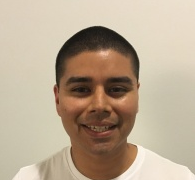
\includegraphics[width=1in,height=1.25in,clip,keepaspectratio]{profile/Marco.png}}]{Marco~Carmona}
  Computer Engineering student at UC Santa Cruz. Responsible for button to base communication using Bluetooth LE standard.
\end{IEEEbiography}

\begin{IEEEbiography}
[{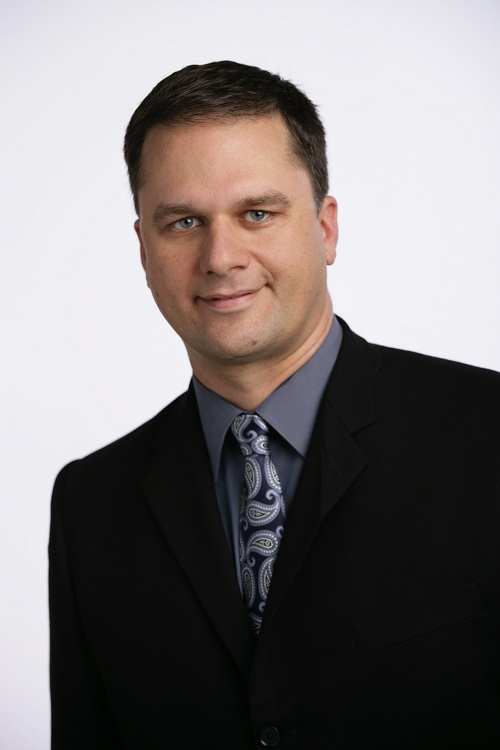
\includegraphics[width=1in,height=1.25in,clip,keepaspectratio]{profile/clchristensen.JPG}}]{Conrad~Christensen}
  Electrical Engineering student at UC Santa Cruz. Responsible for button and base station antenna hardware designs. Enjoys electromagnetic radiation.
\end{IEEEbiography}

\begin{IEEEbiography}
[{
\includegraphics[width=1in,height=1.25in,clip,keepaspectratio]{profile/millk.jpg}}]{Jake~Lee}
  Electrical Engineering student at UC Santa Cruz.  Button hardware design lead.  
\end{IEEEbiography}

\begin{IEEEbiography}
[{
\includegraphics[width=1in,height=1.25in,clip,keepaspectratio]{profile/kevinlee.jpg}}]{Kevin~Lee}
  Computer Engineering (Networking) student at UC Santa Cruz. Lead developer tasked with designing and implementing the Network Application Layer and associated protocols.
\end{IEEEbiography}

\begin{IEEEbiography}
[{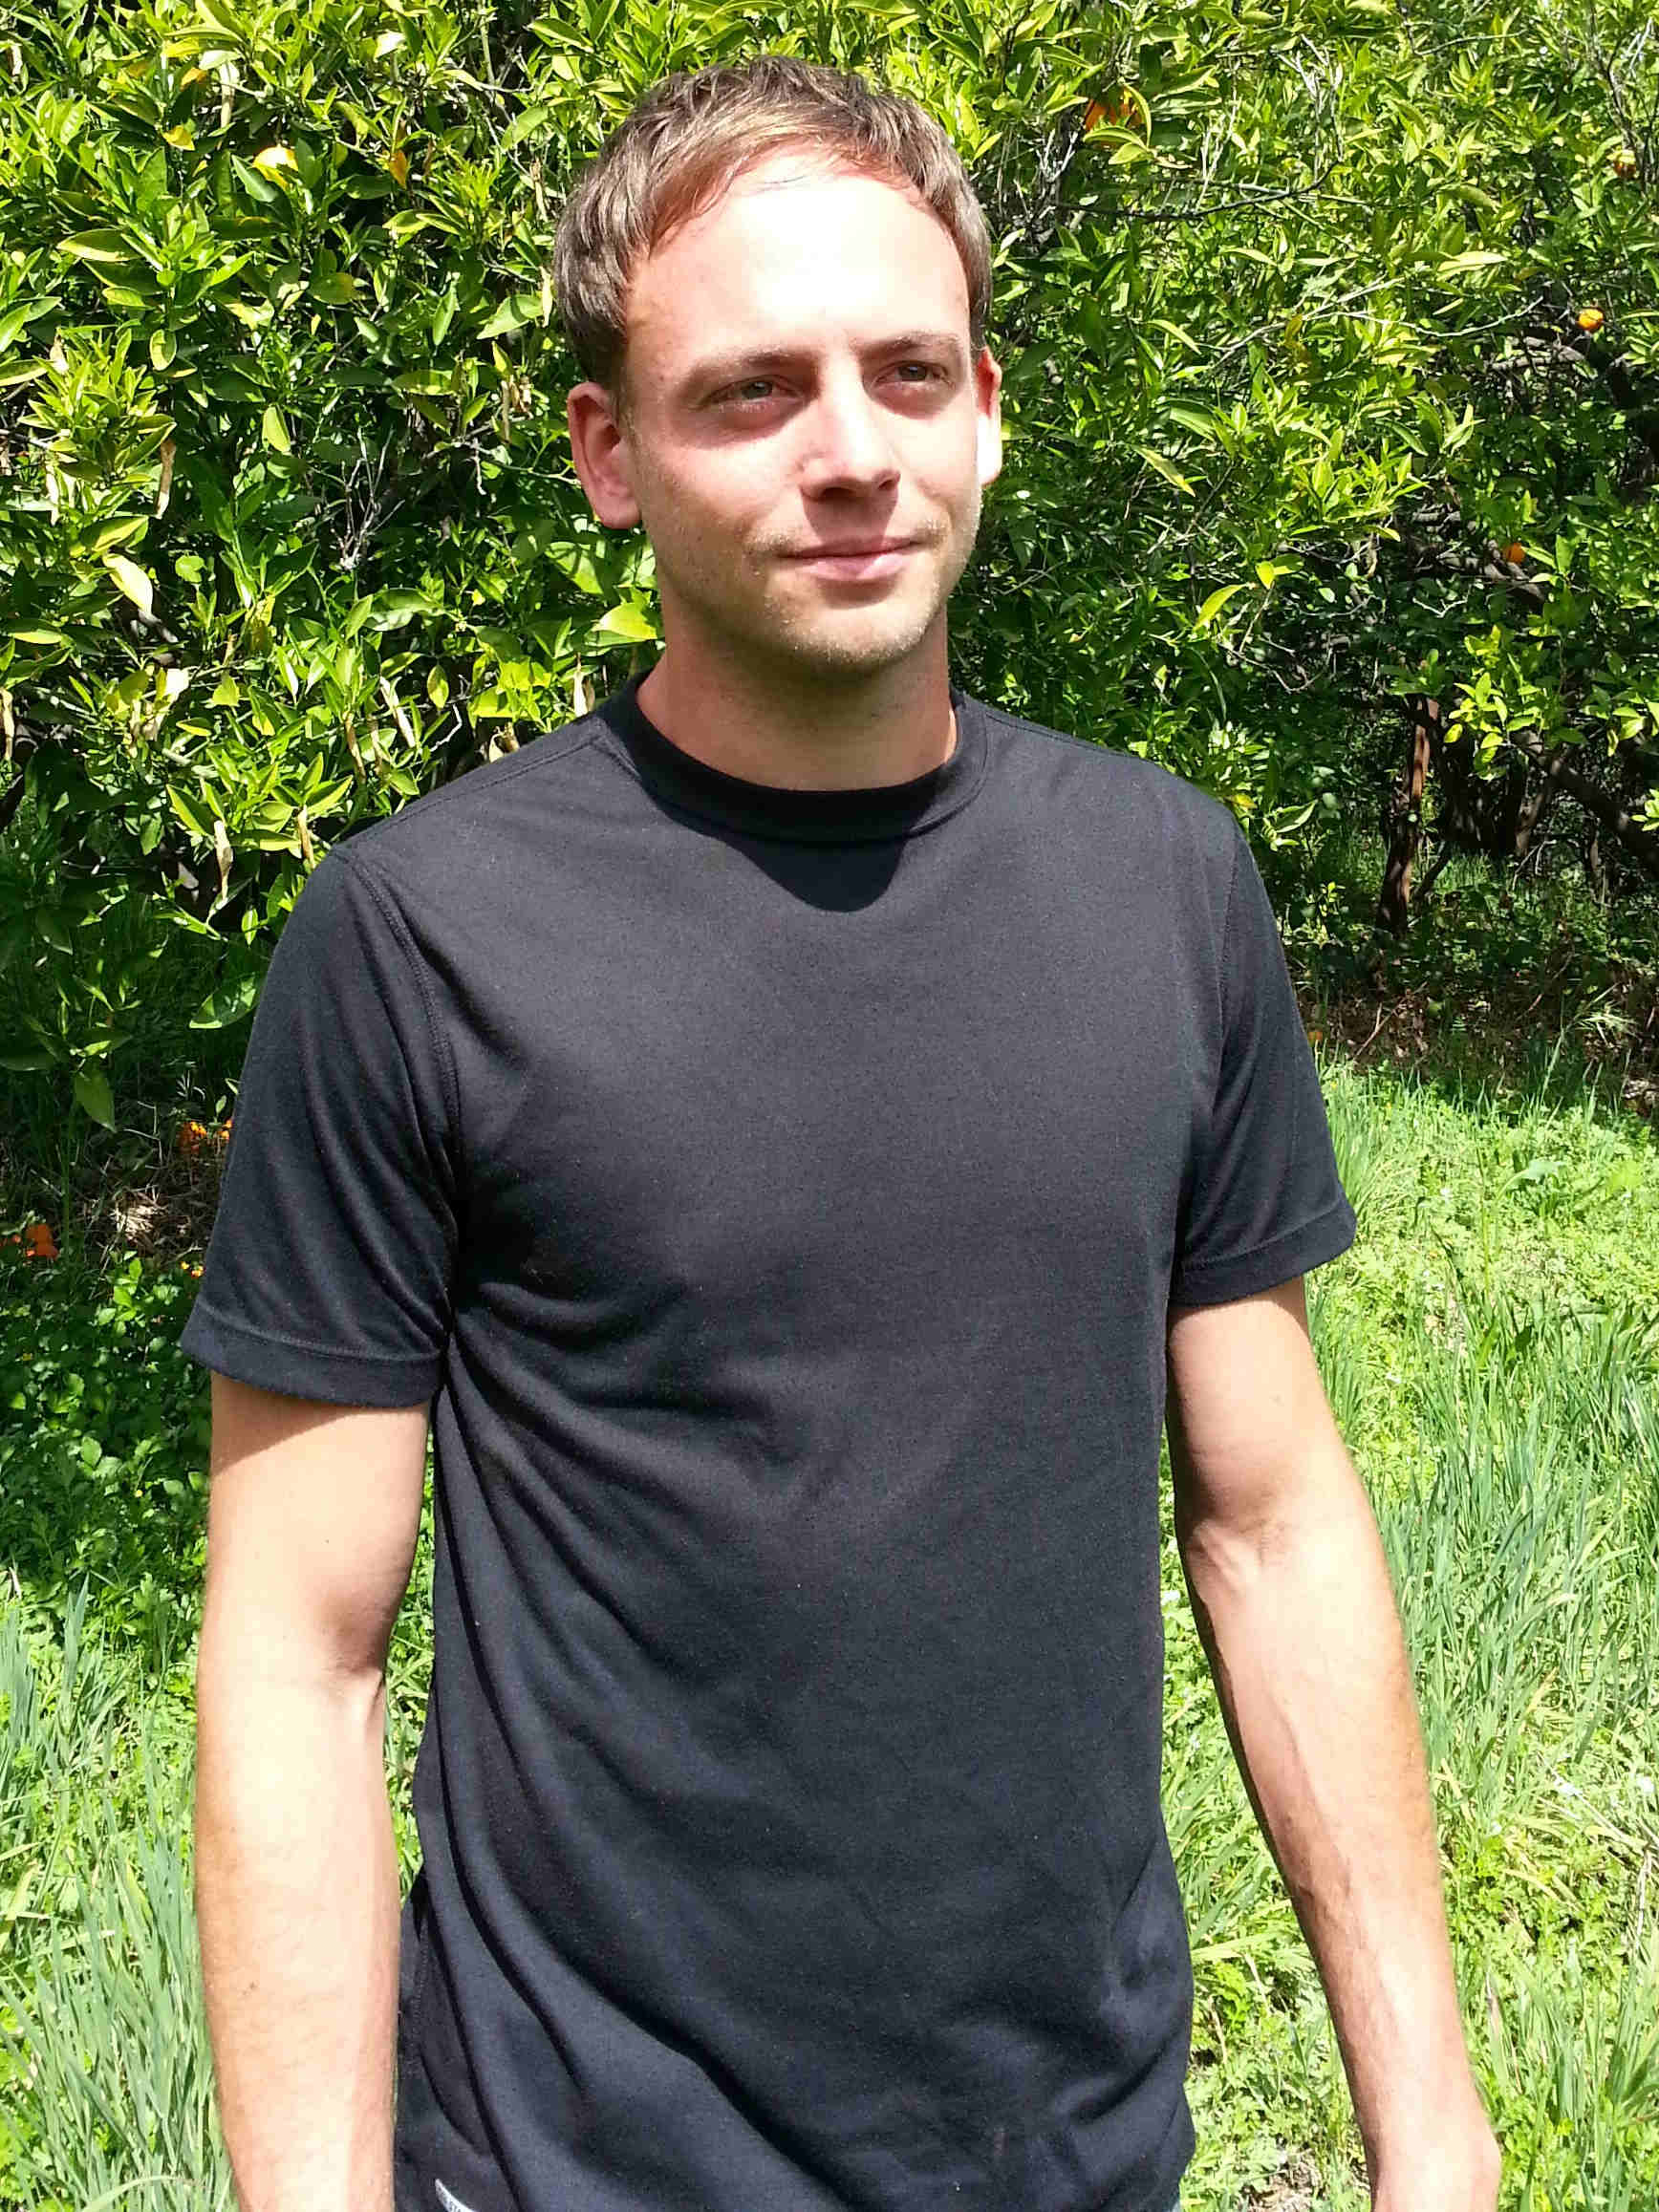
\includegraphics[width=1in,height=1.25in,clip,keepaspectratio]{profile/brian.jpg}}]{Brian~Nichols}
  Computer and Electrical Engineering student at UC Santa Cruz. Lead developer who worked in many areas of the project and the network adaptation layer. 
\end{IEEEbiography}

\begin{IEEEbiography}
[{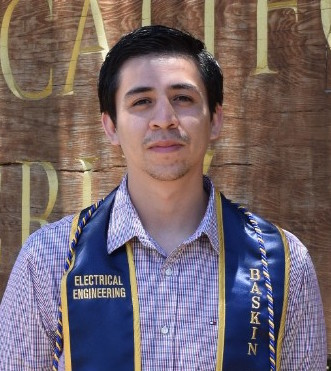
\includegraphics[width=1in,height=1.25in,clip,keepaspectratio]{profile/jsoto.jpeg}}]{Jesus~Soto}
  Electrical Engineering student at UC Santa Cruz. Power Supply and peripheral designer on the hardware team. 
\end{IEEEbiography}

\begin{IEEEbiography}
[{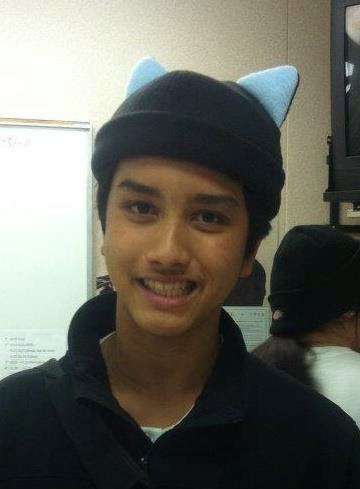
\includegraphics[width=1in,height=1.25in,clip,keepaspectratio]{profile/avalera.jpg}}]{August~Valera}
  Computer Engineering (Systems Programming) and Computer Science student at UC Santa Cruz. Lead UI/UX developer on the software team. Enjoys long walks on the beach.
\end{IEEEbiography}

\begin{IEEEbiography}
[{
\includegraphics[width=1in,height=1.25in,clip,keepaspectratio]{profile/jeffrey.jpg}}]{Jeffrey~Zheng}
  Electrical Engineering student at UC Santa Cruz. Lead designer of the base station hardware.
\end{IEEEbiography}

% You can push biographies down or up by placing
% a \vfill before or after them. The appropriate
% use of \vfill depends on what kind of text is
% on the last page and whether or not the columns
% are being equalized.

%\vfill

% Can be used to pull up biographies so that the bottom of the last one
% is flush with the other column.
%\enlargethispage{-5in}


% that's all folks
\end{document}


